\documentclass[11pt]{article}
\usepackage[a4paper,hmargin=3cm,vmargin=3cm]{geometry}
\usepackage[onehalfspacing]{setspace}
\usepackage[utf8]{inputenc}
\usepackage[T1]{fontenc}
\usepackage[ngerman]{babel}
\usepackage{graphicx}
\usepackage{longtable}
\usepackage{helvet}
\renewcommand{\familydefault}{\sfdefault}
\usepackage{tabto}
\setlength{\parindent}{0em}%kein Einrücken am Absatzanfang
\usepackage{parskip}
\usepackage{fancyhdr}
\pagestyle{fancy}
% Kopfzeile definieren
\fancyhead{}
\fancyhead[R]{Seite \thepage} % Seitenzahl rechts
% Zusätzlicher vertikaler Abstand zwischen Text und Linie
\renewcommand{\headrule}{%
    \vspace{-4pt}% Hier den gewünschten Abstand einstellen
    \hrulefill
}
\fancyfoot{}
\usepackage[font={small, it}]{caption}
\usepackage{float}
\usepackage[ngerman]{varioref}
\usepackage{hyperref}
\hypersetup{
colorlinks=true, % keine farbigen Links (Rahmen werden verwendet)
linkcolor=black,
citecolor=blue,
urlcolor=blue,
linkbordercolor={1 1 1}, % weißer Rahmen um interne Links
citebordercolor={1 1 1}, % weißer Rahmen um Literaturverzeichnis-Links
urlbordercolor={1 1 1} % weißer Rahmen um externe Links
}
\usepackage[noabbrev,german]{cleveref}
\crefname{section}{Kapitel}{Kapiteln}
\crefname{paragraph}{Abschnitt}{Abschnitte}
\crefname{subparagraph}{Abschnitt}{Abschnitte}
\usepackage{enumitem}
\usepackage{xcolor}
\usepackage{mdframed}
\usepackage{pdflscape} 
\widowpenalty=10000
\clubpenalty=10000
\usepackage[backend=biber, style=numeric-comp]{biblatex}
\addbibresource{./bib/DigitalEnergieStand27April.bib}

\begin{document}

\begin{titlepage}
\begin{figure}

\includegraphics[width=5cm,height=3cm,keepaspectratio]{./images/Berner_Fachhochscule.png}
\label{fig:berner_fachhochscule}
\end{figure}
\hrule
\vspace{1.8cm}
\huge
\textbf{Machine Learning in der Energiebranche}

\vspace{0.3cm}
\large
\textbf{Entwicklung und Bewertung von Machine Learning-Modellen für die }\\\textbf{ Prognose des Energieverbrauchs aus Schweizer Trafostationen}

\vspace{2cm}
\textbf{Bachelor Thesis}

\vspace{2.7cm}
\normalsize
eingereicht im Rahmen des Studienganges \tabto {8.5cm}\textbf{Bachelor of Science in}\\
\tabto {8.5cm}\textbf{Wirtschaftsinformatik}

\vspace{0.5cm}
Autorin \tabto {8.5cm}\textbf{Sarah Lea Schürch}

\vspace{0.5cm}
Modul \tabto {8.5cm}\textbf{WBTH -- Bachelor Thesis}

\vspace{0.5cm}
Erstgutachter \tabto {8.5cm}\textbf{Prof. Dr. Eduard Klein}

\vspace{0.5cm}
Zweitgutachter \tabto {8.5cm}\textbf{Prof. Dr. Marcel Gygli}

\vspace{0.5cm}
Datum der Einreichung \tabto {8.5cm}\textbf{22. Mai 2024}

\end{titlepage}
\section*{Abstract}\label{sec:abstract}
Diese Forschungsarbeit umfasst die Entwicklung und Bewertung verschiedener \mbox{Machine} Learning- und Deep Learning-Modelle zur Vorhersage des Energieverbrauchs aus Daten von Schweizer Transformatorenstationen. Die Studie adressiert die Herausforderungen, die bei der Integration von Smart Meter-Echtzeitdaten aufgrund gesetzlicher Bestimmungen und Systemträgheit zu Verzögerungen von bis zu zwei Tagen führen können. Das Ziel dieser Bachelorarbeit war es, Modelle zu erstellen und zu evaluieren, welche diese Datenlücke schliessen und durch die Prognosen Einblicke in zukünftige \mbox{Verbrauchstrends} liefern. 

Nach der Auswahl von sieben Trafostationen basierend auf spezifischen Kriterien wurde eine umfassende exploratorische Datenanalyse (EDA) mit Energieverbrauchsdaten und Meteodaten aus dem Zeitraum 2021 bis 2023 durchgeführt. Verschiedene Variablen aus beiden Datensätzen wurden für die Modellierung herangezogen und es folgte die Prognose der 15-Minuten-Intervalle über 48 Stunden basierend auf den historischen Daten. Es kamen sowohl traditionelle statistische Machine Learning-Modelle (Lineare Regression, SARIMAX, Exponential Smoothing, TBATS) sowie fortschrittliche Deep Learning-Modelle (LSTM- , Transformer-Architektur) zur Anwendung. Abschliessend wurden die Modelle hinsichtlich Vorhersagegenauigkeit, gemessen am MAPE, sowie Komplexität, Ressourceneffizienz und weiterer relevanter Metriken evaluiert.

Die Ergebnisse verdeutlichen, dass fortschrittliche Modelle wie LSTM (MAPE: 3.93~\%) und Transformer (MAPE: 3.93 \%) mit einer guten Ressourceneffizienz zu deutlich präziseren Vorhersagen führen als die betrachteten konventionellen statistischen Methoden. Dennoch sollten statistische Modelle nicht vollständig ausser Acht gelassen werden, insbesondere in Umgebungen, wo keine leistungsfähigen GPUs verfügbar sind, um komplexe Berechnungen effizient durchzuführen. Das Exponential Smoothing-Modell hat mit geringem und das TBATS-Modell mit einem akzeptablen Ressourcenaufwand ebenfalls zu guten Ergebnissen (MAPE: 10 \%) geführt. Überrascht hat das Resultat, dass die Vorhersagegenauigkeit bei den beiden Deep Learning-Modellen ohne die Variablen aus den Meteodaten nur minimal beeinträchtigt wurde. 

Zukünftige Forschungen sollten den Einfluss von Meteodaten auf die Vorhersagegenauigkeit weiter untersuchen und quantifizieren sowie die Anwendbarkeit der Modelle für längere Vorhersagezeiträume und ihre Integration in reale Anwendungsszenarien testen. Diese Arbeit leistet durch die Bewertung verschiedener Prognosemodelle einen wissenschaftlichen Beitrag und unterstützt Energieversorgungsunternehmen bei der effizienten Nutzung von Machine Learning zur Überbrückung von Datenlücken sowie für Energieverbrauchsprognosen.

\newpage
\tableofcontents
\newpage
\listoffigures
\listoftables
\newpage
\section{Einleitung}\label{sec:einleitung}
Die Energieversorgung steht weltweit vor einem Paradigmenwechsel, bedingt durch die zunehmende Dezentralisierung der Energieerzeugung, dem Übergang zu erneuerbaren Energiequellen und steigenden Anforderungen von Verbraucher und Verbraucherinnen \cite{SwissgridNetzZukunft}. Diese Entwicklung stellt herkömmliche Energiemanagementansätze vor neue Herausforderungen, wobei die Implementierung von Smart Metern eine grosse Rolle spielt. Diese intelligenten Zähler sind ein wesentlicher Faktor für eine effizientere und nachhaltigere Energieversorgung, weshalb ihre Einführung als Teil der Energiestrategie 2050 festgelegt wurde \cite{InterviewKlugesSystem}. Angesichts des wachsenden Anteils dezentraler Stromerzeugung und der Notwendigkeit, die Energieeffizienz in der Schweiz zu verbessern, plant die Strategie eine Transformation der bestehenden Energienetze in intelligente Netze, die auch als Smart Grids bekannt sind \cite{BFEIntelligenteNetze}. 


Aufgrund der Energiestrategie 2050 sind die Energieversorger dazu verpflichtet, bis 2027 flächendeckend solche intelligenten Zähler zu installieren. Der Energieverbrauch wird im 15-Minuten-Takt erfasst, wodurch pro Gerät pro Tag 96 Dateneinträge entstehen, was pro Jahr wiederum 35'040 Dateneinträge ergibt \cite{EnergieCHSmartMeter}. Durch diese Erfassung mit Smart Metern fällt für Energieversorger bereits heute wie auch zukünftig eine grosse Menge an Daten an. Diese riesige Menge an Daten gilt es sinnvoll zu verwerten, um den grösstmöglichen Nutzen daraus zu ziehen. Um diesen Nutzen zu erzielen, setzt die vorliegende Arbeit Machine Learning-Modelle ein. Diese Modelle zielen darauf ab, bestehende Datenlücken zu schliessen, eine Prognose des Energieverbrauchs zu erstellen sowie den Einfluss verschiedener Faktoren auf den Energieverbrauch zu erkennen.

\subsection{Ausgangslage}\label{subsec:ausgangslage}
Wie die Einleitung aufzeigt, erzeugt die Einführung von Smart Metern, die im Zuge der Veränderungen im Energiesystem erfolgen, eine enorme Menge an Daten. Diese Daten können im Kontext von Big Data betrachtet werden. Big Data bezieht sich auf Datensätze, die so gross und komplex sind, dass herkömmliche Datenverarbeitungssoftware nicht ausreicht, um sie effektiv zu verarbeiten und zu analysieren \cite{OracleBigData}. Smart Meter generieren kontinuierlich eine grosse Menge Energieverbrauchsdaten, die in Form von Zeitreihen, auch Time-Series genannt, vorliegen. Diese bestehen aus einem Zeitstempel und der Menge an verbrauchter Energie in Kilowatt (kW) oder Kilowattstunden (kWh). In der Schweiz ist es gesetzlich so geregelt, dass der Energieverbrauch alle 15 Minuten erfasst werden darf und einmal täglich an das Energieversorgungsunternehmen übermittelt werden darf \cite{PowernewzSmartMeter}. Diese Smart Meter Daten werden von Energieversorgern auf verschiedenen Ebenen analysiert. Neben der detailliertesten Ebene, Haushaltsebene, werden die Daten auch für Transformatorenstationen aufgezeichnet. Eine Trafostation wandelt elektrische Energie von einem Mittelspannungsnetz in ein Niederspannungsnetz zur allgemeinen Versorgung um \cite{SwissgridNetzebenenTrafostation}. An einer solchen Netzstation sind mehrere Haushalte angeschlossen, deren Energieverbrauch zunehmend durch Smart Meter erfasst wird. Weitere Informationen zum Energiesystem der Schweiz sind in \vref{subsec:energiesystem} zu finden.


Für die vorliegende Arbeit stehen Daten aus sieben solcher Trafostationen über den Zeitraum Januar 2021 bis Dezember 2023 aus einer Schweizer Region zur Verfügung. Die sieben Trafostationen wurden gemeinsam mit dem Energieversorgungsunternehmen basierend auf bestimmten Kriterien definiert. Die Daten der Trafostationen enthalten das Datum, die Uhrzeit sowie der Lastgang in Kilowatt (kW) und sind im 15-Minuten-Takt aufgezeichnet.

Wie bereits durch die Daten-Information-Wissen-Weisheit-Pyramide (DIKW) definiert wird, können Daten ihren Nutzen nur entfalten, wenn daraus Informationen und schlussendlich anwendbares Wissen über die Vergangenheit, Gegenwart oder die Zukunft entstehen \cite{DatacampDIKWPyramid}. Die vorliegende Arbeit setzt genau an diesem Punkt an. Auf die Daten der Trafostationen werden Modelle des maschinellen Lernens, in der weiteren Arbeit auch als Machine Learning bezeichnet, angewendet, um einerseits Datenlücken schliessen zu können und andererseits Vorhersagen des Energieverbrauchs über kurze Zeitspannen aufzustellen. Machine Learning bezeichnet einen Teilbereich der künstlichen Intelligenz, der Computern mit dem Einsatz von Algorithmen die Fähigkeit verleiht, eigenständig aus Daten zu lernen und Entscheidungen sowie Vorhersagen zu generieren, ohne dass sie dafür spezifisch programmiert werden müssen \cite{DatacampMLDefinition}.


Diese Bachelorarbeit wird im Rahmen des Bachelorstudiengangs Wirtschaftsinformatik an der Berner Fachhochschule geschrieben. Die Verfasserin dieser Arbeit stellt einen Bedarf fest, die Eignung verschiedener Machine Learning-Modelle für die Vorhersage von Energieverbrauchsdaten aus Schweizer Trafostationen zu analysieren und zu bewerten.

\subsection{Problemstellung}\label{subsec:problemstellung}
Das zentrale Problem, das in dieser Forschungsarbeit untersucht wird, bezieht sich auf die Nutzung der durch Smart Meter generierten Echtzeitdaten im Energieversorgungssektor. Trotz der Verfügbarkeit grosser Datenmengen gibt es Herausforderungen, um die Daten als Echtzeitdaten zu nutzen. Erstens beschränken Datenschutzbestimmungen die Frequenz, mit der Smart Meter-Daten an Energieversorgungsunternehmen übermittelt werden dürfen. Aufgrund dieser gesetzlichen Bestimmung findet nur einmal pro Tag eine Übermittlung der Daten statt, obwohl die Messungen des Energieverbrauchs im 15-Minuten-Takt erfolgen \cite{bulletinSmartMeterDatenschutz}. Dadurch kann eine Datenlücke von 24 Stunden entstehen. Zweitens führen Verzögerungen bei der Integration dieser Daten aus verschiedenen Quellsystemen in das Dashboard, das zur Visualisierung der Echtzeitdaten dient, zu einer weiteren Lücke. Diese Trägheit der IT-Systeme verursacht eine zusätzliche Datenlücke von 24 Stunden. Aus diesen beiden Gründen kann eine Verzögerung der Dateneinsicht von bis zu zwei Tagen entstehen. Diese Lücke in der zeitnahen Datenverfügbarkeit erschwert es, den aktuellen Energieverbrauch einzuschätzen und zu bewerten.


Die Arbeit verfolgt das übergeordnete Ziel, den Nutzen umfangreicher Datensätze aus Schweizer Transformatorenstationen zu erschliessen, um das Energiemanagement zu verbessern. Angesichts der Verzögerungen bei der Erfassung und Übermittlung von Energieverbrauchsdaten ist dies besonders relevant. Das Hauptziel dieser Bachelorarbeit besteht darin, Machine Learning-Modelle zu entwickeln und anhand definierter Kriterien zu evaluieren, um zeitnahe Prognose zu Energieverbrauchsdaten zu erstellen. Durch diese Modelle soll die erwähnte Datenlücke überbrückt und die Echtzeitdatenverarbeitung verbessert werden, indem Prognosen über den Energieverbrauch in Schweizer Trafostationen für einen Zeitraum von 48 Stunden basierend auf historischen Daten erstellt werden. Zusätzlich bieten diese Modelle die Möglichkeit, durch Vorhersagen über kurze Zeitspannen des Energieverbrauchs wertvolle Einblicke in zukünftige Verbrauchstrends zu gewinnen. Angewendet und bewertet werden sowohl konventionelle statistische Machine Learning-Modelle als auch fortschrittliche Deep Learning-Modelle. Als Ergebnis entsteht ein Leitfaden, der geeignete Modelle für die Vorhersage dieser Zeitreihendaten vorstellt und einen Vergleich der Modelle anhand spezifischer Kriterien bietet.

Die Abgrenzung des Themas ergibt sich durch den Fokus auf die Entwicklung eines Leitfadens mit geeigneten Vorhersagemodellen für den Energieverbrauch unter Verwendung von Machine Learning, ohne andere Anwendungen wie Klassifikationsmodelle zu erforschen. Zudem beschränkt sich die Entwicklung und Bewertung der Modelle auf die Daten aus sieben klar definierten Transformatorenstationen aus einer Schweizer Region. Und schlussendlich konzentriert sich die Arbeit auf Vorhersagen für kurze Zeitspannen, während die Vorhersage langer Zeitspannen nicht behandelt wird.

Die Bedeutung dieser Arbeit ergibt sich aus den aktuellen und zukünftigen Anforderungen, die durch den Wandel hin zu erneuerbaren Energiequellen, die dezentrale Energieerzeugung und den fortschreitenden Digitalisierungsprozess, insbesondere durch die Implementierung von Smart Metern, entstehen. Die Notwendigkeit präziser Vorhersagemodellen wird deutlich, um diesen Herausforderungen wirksam zu begegnen. Sie sollen helfen, die identifizierte Lücke in der Verfügbarkeit von Echtzeit-Daten zu überbrücken und eine proaktive Einsicht in den Energieverbrauch über aktuelle Zeiträume hinaus zu ermöglichen.

\newpage
\subsection{Verwandte Arbeiten}\label{subsec:verwandte_arbeiten}
Im Folgenden werden Studien zusammengefasst, die sich bereits mit ähnlichen verwandten Themen auseinandergesetzt haben. \vref{subsubsec:statistische_machine_learning_modelle_zur_prognose_von_zeitreihendaten} stellt Studien vor, die den Einsatz konventioneller statistischer Machine Learning-Modelle für die Vorhersage von Zeitreihendaten untersucht haben. Anschliessend beschreiben die Studien aus \vref{subsubsec:deep_learning_modelle_zur_prognose_von_zeitreihendaten} den Einsatz fortschrittlicher Deep Learning-Modelle. \vref{subsubsec:forschungsluecke_und_forschungsfrage} präsentiert die identifizierten Forschungslücken sowie die Forschungsfrage.

  

 

\subsubsection{Statistische Machine Learning-Modelle zur Prognose von Zeitreihendaten}\label{subsubsec:statistische_machine_learning_modelle_zur_prognose_von_zeitreihendaten}
Theoretische Entwicklungen in der Zeitreihenanalyse begannen bereits mit stochastischen Prozessen in den 1920er und 1930er Jahren mit den Arbeiten von G.U. Yule und J.Walker \cite{HistoryTimeSeriesAnalysis}, während vor allem die Arbeiten von George Box in den 1970er Jahren als grundlegender Beitrag zur Zeitreihenanalyse gelten. Heute sind konventionelle statistische Methoden sowie einfachere maschinelle Lerntechniken in der Zeitreihenanalyse vorherrschend. Es wird jedoch erwartet, dass mit fortschreitender Rechen- und Datentechnik neue Durchbrüche in der Vorhersage erzielt werden \cite{OreillyZeitreihendatenBuch}.


Zur Vorhersage von Zeitreihendaten bietet die Studie \textit{Machine Learning, Deep Learning and Statistical Analysis for forecasting building energy consumption — A systematic review} aus dem Jahr 2022 einen systematischen Überblick über verschiedene Analysemethoden. Die Studie stellt eine Überprüfung der Forschungsliteratur zu verschiedenen datengetriebenen Ansätzen zur Vorhersage des Energieverbrauchs in Gebäuden dar. Der Artikel konzentriert sich auf die systematische Überprüfung von Machine Learning, Deep Learning und statistischen Analysemethoden, die für die Prognose des Verbrauchs seit 2015 eingesetzt wurden. Die Ergebnisse zeigen Stärken und Schwächen zu verschiedenen Ansätzen wie Random Forest (RF), Support Vector Machine (SVM), Artificial Neural Networks (ANNs), Long-Short-Term Memory (LSTM), Recurrent Neural Networks (RNN), Convolutional Neural Networks (CNN), Lineare Regression (LR) und ARIMA auf. Zum Modell LSTM wird der Vorteil genannt, dass das Model das Problem verschwindender Gradienten löst und Langzeitabhängigkeiten lernt, es jedoch anfällig für Overfitting ist und eine komplexe Struktur aufweist. Zum Modell CNN wird beschrieben, dass es mit einer effizienten Merkmalsextraktion besticht, jedoch grosse Trainingsdatensätze benötigt. Zur linearen Regression wird beschrieben, dass das Model einfach zu verwenden ist und die Ergebnisse einfach zu interpretieren sind. Jedoch ist die Regression nicht geeignet für nichtlineare Datensätze und unzuverlässig bei langfristigen Prognosen. Zum ARIMA-Modell wird beschrieben, dass es sich gut für kurze Vorhersagehorizonte eignet. Die Schwäche ist jedoch, dass es keine Zeitreihen mit saisonalen Komponenten unterstützt. Die Autoren und Autorinnen heben ausserdem hervor, dass es notwendig ist, Modelle weiterzuentwickeln, die mit grossen Datenmengen umgehen können und komplexe nichtlineare Muster in Energieverbrauchsdaten erfassen können \cite{ArticleMLDLSystematicReview} \cite{ChatGPTArticleMLDLSystemicReviewSummary}. Weiter nutzt eine im Jahr 2019 veröffentlichte Studie aus der Schweiz maschinelles Lernen, um den Energieverbrauch und die Energieproduktion unter Einsatz meteorologischer Daten vorherzusagen. In \textit{Machine Learning Techniques for Predicting the Energy Consumption/Production and Its Uncertainties Driven by Meteorological Observations and Forecasts} wurden Methoden wie Multivariate Adaptive Regression Splines (MARS), Quantile Regression Neural Network (QRNN), Kernel Quantile Regression (KQR), Quantile Regression Forest (QRF) und Gradient Boosting Model (GBM) untersucht, die mit traditionellen linearen Modellen verglichen wurden. Die Ergebnisse zeigen, dass Machine Learning-Modelle die Vorhersagegenauigkeit signifikant verbessern und effektiv Unsicherheiten quantifizieren können. Die Studie betont den Nutzen der Kombination verschiedener Machine Learning-Methoden zur Steigerung der Prognosegenauigkeit \cite{ArticleMLEnergyConsumptionAndProduction}.


Die Anwendung des SARIMA-Modells wird in der Studie \textit{Time Series Analysis of Electricity Consumption Forecasting Using ARIMA Model} aus dem Jahr 2021 beleuchtet. Der Artikel konzentriert sich auf die Vorhersage des Stromverbrauchs mit dem ARIMA-Modell, basierend auf historischen Verbrauchsdaten. Ziel der Studie war es, eine genaue Vorhersage für die Planung und Verwaltung des Stromnetzes zu ermöglichen. Dafür wird das ARIMA-Modell angewendet, wobei die Autokorrelationsfunktion (ACF) sowie die partielle Autokorrelationsfunktion (PACF) genutzt werden, um die Modellparameter (p, d, q) zu bestimmen. Die Modellauswahl basiert auf dem geringsten mittleren absoluten prozentualen Fehler (MAPE). Die Ergebnisse identifizieren das saisonale ARIMA-Modell mit den Parametern (0, 1, 6) (1, 1, 6) 7 als das beste Modell, wobei es einen MAPE von 4.3 \% aufweist. Dies deutet auf eine hohe Vorhersagegenauigkeit hin. Die Autoren betonen die Wichtigkeit von genauen Stromverbrauchsprognosen für die Planung und Verwaltung von Smart Grids \cite{ArticleARIMA}. Weiter stellt eine Studie aus dem Jahr 2020 ein neuartiges Prognosesystem vor, das lineare Zeitreihenmodelle und nichtlineare maschinelle Lernmodelle zur Vorhersage des regionalen Energieverbrauchs kombiniert. In der Studie Multistep energy consumption forecasting by metaheuristic optimization of time-series analysis and machine learning wird das SARIMA-Modell für lineare Komponenten und das Least-Squares-Support-Vector-Regression (LSSVR)-Modell für nichtlineare Aspekte genutzt. Die Autoren beschreiben, dass das Modell nur vier Variablen benötigt, wodurch sie die Effizienz dieses Ansatzes unterstreichen. Die Ergebnisse zeigen, dass die vorgeschlagene Kombination von SARIMA und LSSVR genauere Mehrschrittvorhersagen für den Energieverbrauch liefert als einzelne lineare (SARIMA) Modelle, nichtlineare (LSSVR) Modelle und andere hybride Modelle aus vergangenen Studien \cite{ArticleMultistepForecasting}.


Die Methode TBATS wird in der Studie \textit{Effective Short-Term Forecasting for Daily Time Series with Complex Seasonal Patterns} aus dem Jahr 2018 angewendet, die sich auf die Kurzzeitvorhersage von täglichen Zeitreihen mit komplexen saisonalen Mustern konzentriert. Vorhergesagt wird der tägliche Erdgasverbrauch, der mehrere saisonale Muster aufweist. Als Methoden werden insbesondere BATS- und TBATS-Modelle verwendet. Die Ergebnisse zeigen, dass das TBATS-Modell dem BATS-Modell überlegen ist, insbesondere wenn es um die Vorhersage von Zeitreihen mit komplexen saisonalen Mustern geht. Weiter wird gezeigt, dass TBATS weniger Parameter benötigt und somit weniger komplex und schneller in der Ausführung ist. Die Autoren heben die Wichtigkeit der Zerlegung von Zeitreihen in ihre Komponenten hervor, um Einblicke in die Datenstruktur zu erhalten und die Vorhersagegenauigkeit zu verbessern \cite{ArticleShortTermForecasting}.


Weniger Studien wurden hingegen gefunden, welche das Modell Exponential Smoothing auf Zeitreihendaten im Energieverbrauch anwenden. Die Studie Forecasting Electricity Consumption Using Time Series Model aus dem Jahr 2018 beschäftigte sich mit der Vorhersage des Stromverbrauchs an der Universität in Malaysia, bei der verschiedene Zeitreihenmodelle angewendet werden. Das Ziel war es, zukünftige Entwicklungen und Anforderungen des Stromverbrauchs besser planen zu können. In der Studie werden verschiedene Methoden wie gleitende Durchschnitte (SMA), gewichtete gleitende Durchschnitte (WMA), einfache exponentielle Glättung (SES), Holt Linear Trend (HLT), Holt-Winters (HW) und zentrierte gleitende Durchschnitte (CMA) angewendet. Mit den Methoden wurden monatliche Stromverbrauchsdaten von Januar 2011 bis Dezember 2017 analysiert und der Verbrauch für 2018 vorhergesagt. Die Ergebnisse zeigen, dass das Holt-Winters (HW)-Modell den geringsten mittleren absoluten (MAE) und den geringsten mittleren absoluten prozentualen Fehler (MAPE) aufweist. Das CMA-Modell weist hingegen den niedrigsten mittleren quadratischen Fehler (MSE) und die niedrigste Wurzel des mittleren quadratischen Fehlers (RMSE) auf \cite{ArticleForecastingExpSmoothing}.


Zusammenfassend lässt sich sagen, dass die Studien verschiedene Herangehensweisen beleuchten, um Prognosen von Zeitreihendaten aufzustellen. Es wird die Notwendigkeit betont, Modelle zu entwickeln, die mit grossen und komplexen Datensätzen umgehen können und saisonale Muster in den Daten handhaben können. Weiter werden die Vorteile maschineller Lernmethoden gegenüber linearen Modellen präsentiert - besonders in Bezug auf die Vorhersagegenauigkeit.

\subsubsection{Deep Learning-Modelle zur Prognose von Zeitreihendaten}\label{subsubsec:deep_learning_modelle_zur_prognose_von_zeitreihendaten}
Zur Vorhersage von Zeitreihendaten mit Deep Learning-Methoden bietet eine Studie aus dem Jahr 2021 einen Überblick zu verschiedenen Techniken für die Vorhersage des Energieverbrauchs in Gebäuden. Die Studie \textit{A Review of Deep Learning Techniques for Forecasting Energy Use in Buildings} überprüft die Wirksamkeit und das Anwendungspotenzial der Deep Learning-Techniken Autoencoder (AE), Recurrent Neural Networks (RNN) wie Long Short-Term Memory (LSTM) und Gated Recurrent Units (GRU) und Convolutional Neural Networks (CNN), indem eine systematische Überprüfung vorhandener Studien durchgeführt wurde. Die Ergebnisse zeigen, dass Autoencoder oft die beste Prognoseleistung bieten, während RNNs und CNNs die Genauigkeit verbessern können. Deep Learning verbessert generell die Vorhersagegenauigkeit gegenüber traditionellen Methoden - vor allem aufgrund der Fähigkeit, komplexe Muster und Beziehungen in den Daten zu erkennen. Die Studie betont die Wichtigkeit der sorgfältigen Datenauswahl und Modellanpassung, weist jedoch auf noch bestehende Herausforderungen bei der Modellkomplexität und Trainingsdauer hin \cite{ArticleReviewDLTechniques}.


Die Studie Deep learning and transfer learning models of energy consumption forecasting for a building with poor information data aus dem Jahr 2020 untersucht die Anwendung von Sequenz-zu-Sequenz (seq2seq)-Modellen und zweidimensionalen konvolutionalen neuronalen Netzwerken (2D CNNs) auf die Energieverbrauchsprognose in Gebäuden mit unzureichenden Daten. Sie nutzt seq2seq-Modelle, die LSTM für Encoder und Decoder verwenden und 2D CNNs mit einer Aufmerksamkeitsschicht. Die Ergebnisse zeigen eine signifikante Verbesserung der Vorhersagegenauigkeit gegenüber einem einfachen LSTM-Modell, das ausschliesslich auf Daten des Zielgebäudes trainiert wurde. Die Autoren zeigen ausserdem die Bedeutung von Transferlernen in der Energieverbrauchsprognose auf. Modelle, die mit Daten aus einem ähnlichen Kontext vortrainiert sind, können auch in Situationen mit schlechten oder begrenzten Daten nützlich sein \cite{ArticleDLPoorData} \cite{ChatGPTArticleDLPoorDATASummary}.


Die Technik Long Short-Term Memory (LSTM) wird in der Studie \textit{Ensemble Prediction Approach Based on Learning to Statistical Model for Efficient Building Energy Consumption Management} aus dem Jahr 2021 aus Südkorea angewendet. In der Studie wird die Deep Learning-Technik LSTM mit einem statistischen Modell Kalman-Filter kombiniert, um den kurzfristigen Energieverbrauch in Mehrfamilienwohngebäuden vorherzusagen. Die Ergebnisse zeigen, dass das kombinierte Ensemble-Modell aus LSTM und Kalman-Filter in der Lage war, bessere Vorhersageergebnisse zu liefern als die einzelnen Modelle. Das Ensemble-Modell erzielte insbesondere bessere Werte in Bezug auf die Metriken des mittleren absoluten Fehlers (MAE), der Quadratwurzel des mittleren quadratischen Fehlers (RMSE), des mittleren absoluten prozentualen Fehlers (MAPE) sowie des Bestimmtheitsmasses \(R^{2}\) \cite{ArticleEnsembePrediction}.


Mehrere Studien untersuchen den Einsatz von hybriden Deep Learning-Modellen für die Energieverbrauchsprognose. Ein Modell kombiniert LSTM-Netzwerke mit Convolutional Neural Networks (CNN) für die kurzfristige Lastprognose, wobei Daten aus Malaysia und Deutschland verwendet werden. Dieses Modell wird im Artikel \textit{On Short-Term Load Forecasting Using Machine Learning Techniques and a Novel Parallel Deep LSTM-CNN Approach} aus dem Jahr 2022 präsentiert und erzielt eine höhere Genauigkeit als traditionelle Ansätze \cite{ArticleCNNLSTM}. Eine weitere Studie, \textit{A deep learning framework for building energy consumption forecast} aus 2021 setzt einen ähnlichen kCNN-LSTM-Hybridansatz ein, wobei k-Means-Clustering zur Analyse von Energieverbrauchsmustern in einem indischen Gebäude ergänzt wurde. Die Ergebnisse zeigen, dass das kombinierte Modell eine verbesserte Vorhersagegenauigkeit im Vergleich zu anderen aktuellen Energieprognosemodellen aufweist. Die Vorhersagegenauigkeit wurde anhand der Metriken des mittleren absoluten Fehlers (MAE), des mittleren quadratischen Fehlers (MSE), des mittleren absoluten prozentualen Fehlers (MAPE) sowie der Quadratwurzel des mittleren quadratischen Fehlers (RMSE) bewertet \cite{ArticleDLForecast}. Ebenfalls verwendet die Studie \textit{Multi-Step Short-Term Power Consumption Forecasting with a Hybrid Deep Learning Strategy} aus dem Jahr 2018 ein hybrides Modell aus CNNs und LSTM, um präzisere Vorhersagen zu erreichen. Der Fokus liegt auf der Entwicklung eines Frameworks zur Prognose des kurzfristigen Energieverbrauchs, das die Stärken von CNNs zur Merkmalsextraktion und LSTM zur Vorhersage kombiniert. Das Modell übertrifft herkömmliche Methoden wie Support Vectore Machine-Methode (SVM) und ARIMA \cite{ArticleMultiStepHybridForecast}.


Der Artikel \textit{Transformer-Based Model for Electrical Load Forecasting} aus dem Jahr 2022 untersucht die Anwendung der Transformer-Architektur zur Vorhersage des elektrischen Lastverbrauchs, die ursprünglich aus der Verarbeitung natürlicher Sprache (NLP) stammt. Die Transformer-Technik hat sich im Bereich der natürlichen Sprachverarbeitung aufgrund der parallelen Verarbeitungsfähigkeit und Genauigkeit durchgesetzt. Diese Studie untersucht die Anpassung der Transformer-Architektur für Zeitreihendaten des Lastverbrauchs. Die Ergebnisse zeigen, dass die Anpassung der Architektur an Zeitreihendaten herkömmliche Seq2Seq-Modelle (RNN) in der Leistung übertreffen und effizient mit kontextuellen Daten umgehen kann \cite{ArticleTransformer}. Auch die Studie \textit{ETSformer: Exponential Smoothing Transformers for Time-series Forecasting}, ebenfalls aus dem Jahr 2022, nutzt eine neue Transformer-Architektur für die Zeitreihenprognose. Die Studie setzt auf die Kombination mit dem Exponential Smoothing Modell zur Verbesserung der Genauigkeit und Effizienz. Die Ergebnisse zeigen eine überlegene Leistung der Architektur im Vergleich zu bestehenden Ansätzen bezüglich der Effektivität, der hohen Genauigkeit sowie der besseren Interpretierbarkeit \cite{ArticleTransformerExpSmoothing}.


Zusammenfassend haben die Studien gezeigt, dass Deep Learning-Methoden effektiv für die Vorhersage von Zeitreihendaten eingesetzt werden können. Die Modelle bieten eine signifikante Verbesserung der Vorhersagegenauigkeit in Anwendungen zur Energieverbrauchsprognose in Gebäuden gegenüber traditionellen Methoden. Insbesondere die Fähigkeit, komplexe Muster und saisonale Komponenten in den Daten zu erkennen und zu modellieren, trägt wesentlich zur Verbesserung der Prognosegenauigkeit bei. Weiter zeigen die Studien, dass der Einsatz der Deep Learning-Techniken auch ein besseres Verständnis und eine bessere Interpretierbarkeit der Zeitreihen ermöglicht. Diese Studien bestärken die Annahme, dass die Kombination von maschinellem Lernen und speziell angepassten Deep Learning-Architekturen für die Zeitreihenprognose vielversprechend sind.

\subsubsection{Forschungslücke und Forschungsfrage}\label{subsubsec:forschungsluecke_und_forschungsfrage}
Zusammenfassend lässt sich sagen, dass es 7 grosse Forschungslücken gibt:

\begin{enumerate}
    \item Integration und Analyse von Echtzeitdaten: Die Herausforderung bei der Integration von Echtzeitdaten aus Smart Metern und deren Nutzung für eine präzise Energieverbrauchsvorhersage sind noch nicht vollständig gelöst.

    \item Methodik: Die meisten Studien verwenden einen Ansatz und vergleichen diesen gegenüber einem anderen Modell oder untersuchen systematisch die Forschungsliteratur. Nur wenige Studien vergleichen die Leistung und die Effizienz der verschiedenen State-of-the-Art-Modelle im Vergleich für Zeitreihendaten umfassend.

    \item Vorhersagezeitraum: Die meisten Studien berücksichtigen die kurzfristige Energieverbrauchsprognose, jedoch nicht die langfristige Vorhersage.

    \item Bilanzierung von Energieflüssen: Die meisten Studien verwenden Energieverbrauchsdaten, berücksichtigen jedoch nicht die Energieproduktion durch Haushalte.

    \item Einflussfaktoren: Wenige Studien berücksichtigen zusätzlich zu den Daten meteorologische Einflüsse.

    \item Multidimensionale Evaluationskriterien: Die meisten Studien fokussieren sich auf die Vorhersagegenauigkeit. Nur wenige Studien berücksichtigen den Ressourcenaufwand sowie die Modellkomplexität.

    \item Reale Anwendungsszenarien: Keine gefundene Studie testet die Modelle mit Daten aus Transformatorenstationen in  realen Anwendungsszenarien, um ihre praktische Tauglichkeit zu bewerten.

\end{enumerate}

Die Erarbeitung dieser Studie trägt dazu bei, einen Beitrag zu den Forschungslücken 1), 2) und 6) zu leisten, indem sie die folgende Forschungsfrage anhand von Energieverbrauchsdaten beantwortet, die aus sieben Schweizer Transformatorenstationen stammen:

\begin{mdframed}[backgroundcolor=gray!20, innertopmargin=10pt, innerbottommargin=10pt, innerleftmargin=10pt, innerrightmargin=10pt, rightmargin=15pt, skipabove=10pt, skipbelow=10pt, linewidth=0pt]
\textit{FF: Welche Machine Learning-Modelle eignen sich am besten für die Prognose von Zeitreihendaten des Energieverbrauchs aus Schweizer Transformatorenstationen?}

\end{mdframed}

Meteorologische Daten werden in einige der Modelle zusätzlich integriert, wodurch zur Forschungslücke 5) bis zu einem gewissen Grad einen Beitrag geleistet wird. Zur Forschungslücke 7) wird ebenfalls teilweise beigetragen, indem die verwendeten Daten aus Transformatorenstationen stammen.

Obwohl das Thema bereits in verschiedenen Studien behandelt wurde, erweitert diese Arbeit die bestehende Literatur durch eine fokussierte Analyse der Vorhersagegenauigkeit und praktischen Implementierung der Modelle mit Schweizer Energieverbrauchsdaten. 

\newpage

\subsection{Methodik}\label{subsec:methodik}
Die methodische Herangehensweise zielte darauf ab, durch die Analyse von Echtzeitdaten des Energieverbrauchs aus Schweizer Trafostationen präzise Machine Learning-Vorhersagemodelle zu erstellen, die anschliessend basierend auf definierten Kriterien bewertet und verglichen werden können. 

In einem ersten Schritt wurden gemeinsam mit dem Energieversorgungsunternehmen 7~Trafostationen definiert, von denen die Daten in die Modelle einfliessen sollen. Die Trafostationen wurden nach Kriterien wie der Erreichbarkeit der Zähler, einem Ausrollungsgrad von Smart Metern über 50 \% und der zukünftigen Planung von Photovoltaikanlagen und Elektromobilitätsstationen im Gebiet der Trafostation, definiert. Die Energieverbrauchsdaten wurden über den Zeitraum Januar 2021 bis Dezember 2023 zur Verfügung gestellt. Im zweiten Schritt wurde eine Literaturrecherche durchgeführt, um den aktuellen Stand in der Anwendung verschiedener Machine Learning-Ansätze aufzuzeigen. Ausserdem wurden die erforderlichen Rechenressourcen beschafft, um die anschliessende Anwendung der Machine Learning-Modelle durchzuführen. Die zur Verfügung stehenden Ressourcen sind in \vref{sec:ergebnisse} beschrieben. Im dritten Schritt folgte die Datenbearbeitung und -bereinigung sowie eine exploratorische Datenanalyse (EDA), um ein besseres Verständnis über die Zeitreihendaten zu erlangen.


Nach dem Ausgeben wichtiger Kennzahlen wie dem Mittelwert und den Quartilen anhand der deskriptiven Statistik wurden die Daten auf fehlende Werte überprüft. Die Datenanalyse umfasste die Visualisierung durch Histogramme zur Erfassung der Datensatzverteilung, Box-Plots zur Identifizierung von Ausreissern und Liniendiagramme zur Erkennung grundlegender Trends. Weiter wurde der Datensatz für eine detailliertere Zeitreihenanalyse auf täglicher, wöchentlicher und monatlicher Basis aggregiert. Autokorrelationsdiagramme und die Dekomposition der Zeitreihen in Trend, Saisonalität und Residuen halfen, periodische Muster und saisonale Effekte zu verstehen. Diese Schritte waren für die anschliessende Modellierung und Vorhersage wichtig. Abschliessend wurde die Stationarität der Daten mit dem Augmented-Dickey-Fuller (ADF)-Test überprüft, da einige Modelle wie beispielsweise SARIMA eine Stationariät der Daten erwarten. Auch wurden in diesem Arbeitsschritt die Meteodaten an die Energieverbrauchsdaten angepasst. Die Daten wurden von der Meteotest AG zu Forschungszwecken zur Verfügung gestellt und stammen von der \href{https://meteonorm.com/}{Meteonorm-Software}. Die Daten umfassen Messungen im 15-Minuten-Intervall aus derselben Schweizer Region wie die Trafostationen über den gleichen Zeitraum. Der Datensatz enthält neben dem Zeitstempel die Variablen Globalstrahlung, Sonnenhöhe, extraterrestrische Strahlung, stündliche Strahlungswerte, Diffusstrahlung, Diffusstrahlung auf geneigte Flächen, Direktnormalstrahlung, Lufttemperatur, Windgeschwindigkeit, Schönwetterstrahlung, Taupunkttemperatur und die theoretische Stromproduktion einer Photovoltaikanlage.  Abschliessend wurde eine Korrelationsmatrix und eine Heatmap erstellt, um die Beziehungen zwischen den verschiedenen Variablen und dem Lastgang zu analysieren. Dies diente dazu, die Variablen für die Integration in die Modelle zu identifizieren, welche die stärkste Korrelation mit Energieverbrauchsdaten aufweisen. In dieser Arbeit werden die Begriffe Variablen und Features nachfolgend gleichbedeutend verwendet. Detailliertere Ausführungen zur Datenbereinigung und zur anschliessenden exploratorischen Datenanalyse sind in \vref{subsec:explorative_datenanalyse__eda_} zu finden. 

Als vierter Schritt folgte die Anwendung der Machine Learning-Modelle, um die Daten vorherzusagen. Die Regressionsanalyse diente als Baseline, ergänzt durch SARIMA, TBATS und Exponential Smoothing für saisonale Zeitreihendaten sowie fortschrittliche LSTM- und Transformer-Modelle. Ziel war es, die Modellgenauigkeit durch Einbeziehung zusätzlicher Variablen wie etwa aus Meteodaten zu verbessern. Das genaue Vorgehen bei der Anwendung der verschiedenen Modelle ist in \vref{subsec:anwendung_der_machine_learning_modelle} zu finden. Als letzter Schritt folgte die Evaluation. Diese zielte darauf ab, die effektivsten Modelle für präzise Energieverbrauchsprognosen zu identifizieren. Das primäre Kriterium war die Vorhersagegenauigkeit über zwei Tage. Dies beinhaltet insbesondere die Fähigkeit eines Modells, den Energieverbrauch mit möglichst geringer Abweichung von den realen Werten vorherzusagen. Die genauen Kriterien und der Vergleich der Modelle sind in \vref{subsec:evaluation_und_vergleich_der_machine_learning_modelle} zu finden. Die exploratorische Datenanalyse und insbesondere die Anwendung der Modelle wurde zu Beginn mit einem kleineren Datensatz durchgeführt, um die Modellkonfigurationen zu optimieren. Anschliessend wurden schrittweise weitere Daten und Variablen hinzugefügt.

Die Arbeit beginnt in \vref{sec:einleitung} mit einer Einführung, die den Hintergrund der Nutzung von Machine Learning zur Energieverbrauchsprognose in Schweizer Trafostationen beleuchtet, beschreibt die Problemstellung, verwandte Arbeiten sowie die Forschungsfrage. Sie skizziert weiter die Methodik, die von der Datenauswahl bis zur Modellentwicklung und -evaluation reicht. Der theoretische Rahmen in \vref{sec:theoretischer_hintergrund} gibt einen kurzen Überblick über das Energiesystem, Zeitreihendaten und die angewandten Machine Learning-Modelle. Die Ergebnisse umfassen mit \vref{subsec:explorative_datenanalyse__eda_} die Datenbereinigung und die explorative Datenanalyse (EDA), mit \vref{subsec:anwendung_der_machine_learning_modelle} die Anwendung der einzelnen Modelle sowie mit \vref{subsec:evaluation_und_vergleich_der_machine_learning_modelle} die Evaluation und der Vergleich hinsichtlich der definierten Kriterien. Im Anschluss folgt in \vref{sec:diskussion_und_fazit} eine Diskussion zur Effektivität der Modelle, zum Nutzen für die Energiebranche und ein Ausblick. Die Arbeit beinhaltet ausserdem in \vref{sec:glossar} ein Glossar mit relevanten Begriffen. Diese Arbeit soll somit neben dem praktischen Nutzen für Energieversorgungsunternehmen und dem wissenschaftlichen Beitrag die Forschungsfrage beantworten, welche Machine Learning-Modelle sich am besten für die Prognose von Zeitreihendaten des Energieverbrauchs aus Schweizer Transformatorenstationen eignen. 

\newpage
\section{Theoretischer Hintergrund}\label{sec:theoretischer_hintergrund}
Dieses Kapitel legt mit einer kurzen Einführung in das Energiesystem der Schweiz und zu Zeitreihendaten den theoretischen Grundstein für die Verarbeitung von Energieverbrauchsdaten. Abschliessend werden die Machine Learning-Modelle vorgestellt, was entscheidend zur Nachvollziehbarkeit der später präsentierten Ergebnisse beiträgt.

\subsection{Energiesystem}\label{subsec:energiesystem}
Die Schweiz hat sich mit der Energiestrategie 2050 dazu verpflichtet, die Energieeffizienz zu steigern, den Energieverbrauch zu reduzieren und den Anteil erneuerbarer Energien zu erhöhen \cite{GrundsatzEnergiepolitik}. Ein wesentlicher Bestandteil dieser intelligenten Netze sind Smart Meter. Seit ihrer gesetzlich vorgeschriebenen Einführung im Jahr 2018 symbolisieren sie den Übergang zur Digitalisierung der Energieversorgung \cite{GrundsatzEnergiepolitik}. Die Energieversorgungsunternehmen sind verpflichtet, bis 2027 die Haushalte flächendeckend, bis 80 \%, mit diesen intelligenten Zählern auszustatten \cite{ZHAWSmartMetering}. Smart Meter sind intelligente Stromzähler, die den Energieverbrauch in Echtzeit erfassen und übermitteln können. In der Schweiz wird der Energieverbrauch im 15-Minuten-Takt erfasst, wobei die Übermittlung der Daten an das Energieversorgungsunternehmen aufgrund von Datenschutzbestimmungen einmal pro Tag erfolgt \cite{bulletinSmartMeterDatenschutz}. Der Energieverbrauch wird üblicherweise in Kilowattstunden (kWh) gemessen. Dies entspricht der Energiemenge, die ein Gerät mit einer Leistung von einem Kilowatt über eine Stunde verbraucht \cite{Paschotta2010}. Kilowatt (kW) hingegen ist eine Einheit für die Leistung \cite{EKZKWvsKWH}. Für das Verständnis der Rolle von Smart Metern im Energiemanagement ist es wichtig, die Bedeutung der 50-Hertz-Frequenz im Stromnetz zu kennen. Das schweizerische sowie die europäischen Stromnetze arbeiten mit dieser festgelegten Frequenz von 50 Hertz (Hz), welche die Anzahl der Wechselstromzyklen pro Sekunde angibt. Diese Frequenz ist ausschlaggebend für die Netzstabilität und Zuverlässigkeit der Stromversorgung \cite{IWB2022}. Dafür ist ein Gleichgewicht zwischen Energieerzeugung und -verbrauch notwendig \cite{SwissgridNetzstabilität}. Abweichungen von dieser Frequenz können zu Netzinstabilitäten und gravierenden Stromausfällen, oft als Blackout bezeichnet, führen \cite{Axpo2022}. Das Energiesystem der Schweiz besteht aus sieben Ebenen, wobei die Hochspannungsleitungen die Energie über weite Strecken transportieren und die Verteilung an die Endverbraucher und Endverbraucherinnen über Niederspannungsleitungen erfolgt \cite{SwissgridNetzebenenTrafostation}. Transformatorenstationen, auch Trafostationen oder Netzstationen genannt, sind im Energiesystem installiert, um die Spannung der elektrischen Energie sowohl für die lokale Verteilung anzupassen als auch für den Transport über weite Strecken.

\subsection{Zeitreihendaten}\label{subsec:zeitreihendaten}
In der heutigen modernen Welt werden riesige Mengen an Daten erzeugt, die unter dem Stichwort Big Data zusammengefasst werden können \cite{OracleBigData}. Eine Art von Daten, sogenannte Zeitreihendaten, sind besonders in Bereichen wie der Meteorologie, Finanzen, Gesundheitsgeräten, Sensoren wie beispielsweise in Internet of Things-Geräten oder in der Entwicklung smarter Städte von Bedeutung, da sie Veränderungen und Trends über die Zeit hinweg aufzeigen \cite{OreillyZeitreihendatenBuch}. In die Kategorie der Zeitreihendaten fallen auch die Energieverbrauchsdaten, die durch Smart Meter im Energiesektor erfasst werden. Zeitreihendaten, auch Time Series genannt, beziehen sich auf Beobachtungen, die in regelmässigen Abständen im Laufe der Zeit aufgezeichnet werden \cite{OreillyZeitreihendatenBuch}. Sie bestehen im Grunde genommen aus einem Zeitstempel und einem dazugehörigen Wert, wie in Abbildung \ref{fig:zeitreihendaten_mit_zeitstempel_und_lastgang_in_kilowatt} zu sehen ist. Die optimale Speicherung von Zeitreihendaten erfordert Systeme, die grosse Datenvolumina effizient verarbeiten können und eine schnelle Abfrage ermöglichen. Geeignet für die Speicherung solcher Daten sind Zeitreihendatenbanken, die für Zeitstempeldaten optimiert sind und mit einer effizienten Speicherung und Abfragemöglichkeit trumpfen \cite{DunningFriedman2014}. Vertreter dieses Datenbanktyps sind beispielsweise InfluxDB, TimescaleDB oder Prometheus.


\begin{figure}[h]
\centering
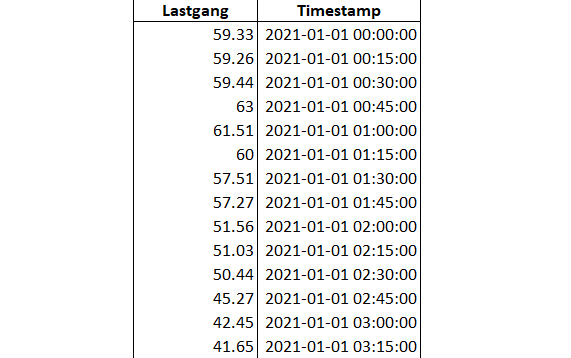
\includegraphics[width=10.25cm,keepaspectratio]{./images/Zeitreihendaten_mit_Zeitstempel_und_Last.png}
\caption{Zeitreihendaten mit Zeitstempel und Lastgang in Kilowatt}
\small~\textit{(Quelle: Eigene Darstellung).}
\label{fig:zeitreihendaten_mit_zeitstempel_und_lastgang_in_kilowatt}
\end{figure}
Zeitreihendaten können saisonale Muster, Trends und Zyklen aufweisen und erfordern spezielle Analysemethoden, welche die Zeitabhängigkeit berücksichtigen. Die Analyse von Zeitreihendaten beinhaltet oft Methoden zur Trend- und Mustererkennung, Vorhersage und Anomalieerkennung \cite{OreillyZeitreihendatenBuch}. Dadurch unterscheidet sie sich von anderen analytischen Ansätzen. Ziel ist es, Muster, Trends und saisonale Schwankungen im Laufe der Zeit zu entdecken und diese Komponenten bei der anschliessenden Vorhersage zu berücksichtigen.

\subsection{Machine Learning-Modelle zur Prognose von Zeitreihendaten}\label{subsec:machine_learning_modelle_zur_prognose_von_zeitreihendaten}
Zur Beantwortung der in \vref{subsubsec:forschungsluecke_und_forschungsfrage} genannten Fragestellung werden Machine Learning-Ansätze angewendet, um präzise Vorhersagemodelle zu ermöglichen. Dies umfasst Methoden des Supervised Learnings. Bei diesem Ansatz lernen die Modelle mithilfe gelabelter Trainingsdaten die Beziehung zwischen Eingabedaten und ihren zugehörigen Ausgaben. Beispiele sind Klassifizierung und Regression \cite{IBMSupervisedUnsupervisedLearning}. Im Gegensatz dazu werden bei einem Ansatz mit unsupervised Learning die Modelle mit ungelabelten Daten trainiert, damit sie eigenständig Muster und Strukturen in den Daten erkennen. Ein Beispiel sind Clusteringsaufgaben \cite{IBMSupervisedUnsupervisedLearning}. In diesem Kapitel wird die theoretische Grundlage der angewendeten Ansätze umrissen.

\subsubsection{Lineare Regression}\label{subsubsec:lineare_regression}
Die lineare Regression modelliert die Beziehung zwischen einer abhängigen Variablen und einer oder mehreren unabhängigen Variablen. Die Gleichung dafür ist \mbox{y = xw + b}. Dabei ist y die vorhergesagte Variable, x die unabhängige Variable, w die Gewichtung und b die Verzerrung \cite{ScribbrLineareRegression}.


Ein Beispiel, wie eine lineare Regression mit Python durchgeführt werden kann, ist in \vref{sec:quellcode_der_machine_learning__und_deep_learning_modelle} zu sehen. Die lineare Regression wird als Bezugspunkt verwendet, um potenzielle Verbesserungen, die durch komplexere Algorithmen erzielt werden, zu erkennen \cite{OreillyDataScienceBuch}. Die Ergebnisse zur linearen Regression sind in \vref{subsubsec:lineare_regression} zu finden.

\subsubsection{SARIMAX}\label{subsubsec:sarimax}
(S)ARIMA(X) steht für (Saisonale) Autoregressive Integrierte Gleitende Durchschnitte (mit exogenen Variablen). Die Methode stammt aus der bekannten ARIMA-Familie, berücksichtigt aber auch die Saisonalität in den Daten und lässt exogene Variablen zu. Das Modell eignet sich gut für Zeitreihen, die sowohl saisonale als auch nicht saisonale Muster aufweisen und bei denen zusätzlich externe Einflussfaktoren berücksichtigt werden sollen \cite{DatacampSARIMAForecasting}. Die Erstellung eines SARIMAX-Modelles mit Python ist im Anhang in \vref{sec:quellcode_der_machine_learning__und_deep_learning_modelle} abgebildet. Hervorzuheben ist die Code-Zeile, in der das Modell erstellt wird:


\begin{mdframed}[backgroundcolor=gray!20, innertopmargin=10pt, innerbottommargin=10pt, innerleftmargin=10pt, innerrightmargin=10pt, rightmargin=15pt, skipabove=10pt, skipbelow=10pt, linewidth=0pt]
\textit{\# Erstellen \& Anpassen des SARIMAX-Modells und Training}\\
\textit{\# SARIMAX-Modell mit ARIMA(1,0,0) und saisonaler Ordnung (1,0,0,96)}\\
\textit{model = sm.tsa.SARIMAX(y\_train, exog=X\_train, order=(1,0,0), }\\ \textit{seasonal\_order=(1,0,0,96), enforce\_stationarity=False, }\\ \textit{enforce\_invertibility=False)}\\
\textit{results = model.fit()}

\end{mdframed}

Die externen Variablen werden zuerst in 'X\_train' gespeichert. Bei der Modellerstellung werden sie mit 'exog=' aufgerufen. Die Komponente 'order' besteht aus (p, d, q), während die Komponente 'seasonal\_order' aus (P, D, Q, s) besteht \cite{sktimeDocuSARIMA}. Die Bestimmung der Parameter sowie die Ergebnisse zu diesem Modell sind in \vref{subsubsec:sarimax} dargestellt.

\subsubsection{Exponential Smoothing}\label{subsubsec:exponential_smoothing}
Bei Exponential Smoothing, auch exponentielle Glättung genannt, wird den jüngeren Beobachtungen ein grösseres Gewicht beigemessen als den älteren Beobachtungen. Ziel dieser exponentiellen Glättung ist es, dass die Prognose weniger durch zufällige Schwankungen in den Daten beeinflusst wird \cite{DatacampSARIMAForecasting}. 


Das Simple Exponential Smoothing geht von einer Zeitreihe ohne Trend und Saisonalität aus und erstellt Prognosen anhand eines gewichteten Durchschnitts der vorangegangenen Beobachtungen und Vorhersagen für die aktuelle Periode. Beim Double Exponential Smoothing, auch Lineare Exponential Smoothing von Holt genannt, wird ein linearer Trend berücksichtigt, aber ohne saisonale Muster. Das Triple Exponential Smoothing, oder Holt-Winter-Modell, wird verwendet, wenn die Daten sowohl einen Trend als auch eine saisonale Komponente aufweisen.   Die Anwendung eines Triple Exponential Smoothing-Modells mit Python ist im Anhang in \vref{sec:quellcode_der_machine_learning__und_deep_learning_modelle} zu sehen.

\begin{mdframed}[backgroundcolor=gray!20, innertopmargin=10pt, innerbottommargin=10pt, innerleftmargin=10pt, innerrightmargin=10pt, rightmargin=15pt, skipabove=10pt, skipbelow=10pt, linewidth=0pt]
\textit{\# Modellinitialisierung und Training}\\
\textit{\# Berücksichtigung additiver saisonaler Komponente und 96 als Periode für tägliche Saisonalität (bei 15-Minuten-Intervalle)}\\
\textit{model = ExponentialSmoothing(train\_data, seasonal='add', seasonal\_periods=96)}\\
\textit{fitted\_model = model.fit()}

\end{mdframed}

Nach der Aufteilung in Trainings- und Testdatensatz folgt die Erstellung eines Triple Exponential Smoothing-Modells. Bei der Modellerstellung geben 'trend='add'' und 'seasonal='add'' an, dass die Komponenten additiv behandelt werden. Additiv bedeutet, dass die saisonalen Schwankungen als konstante Absolutwerte über die Zeit angenommen werden \cite{MLMasteryExpSmoothing}. Mit der 'fit()'-Methode wird das Modell anschliessend an die Daten angepasst, wobei die optimalen Parameter des Modells auf die Daten berechnet wird. Das \vref{subsubsec:exponential_smoothing} präsentiert die Resultate zu diesem Modell. 

\subsubsection{TBATS}\label{subsubsec:tbats}
TBATS steht für Trigonometrische Saisonalität, Box-Cox-Transformation, ARMA-Fehler, Trend und Saisonale Komponenten. Das Modell wurde speziell für den Umgang mit komplexen saisonalen Mustern entwickelt \cite{DatacampSARIMAForecasting}. 


Die trigonometrische Saisonalität ermöglicht die Modellierung von saisonalen Mustern mit variabler Länge. Zum Beispiel können tägliche und wöchentliche Muster in Energieverbrauchsdaten erfasst werden. Durch die Box-Cox-Transformation werden die Zeitreihen transformiert, um Varianzstabilität zu gewährleisten. Dies ist besonders wichtig, wenn die Varianz nicht konstant ist. So kann beispielsweise die Nicht-Stationarität der Varianz von Energieverbrauchsdaten stabilisiert werden. Die Komponente des ARMA-Fehlers bedeutet, dass ein ARMA-Modell für die Fehlerterme verwendet wird, welches die Autokorrelation berücksichtigt. Die Trend-Komponente ermöglicht es dem Modell, sowohl stabile als auch sich zufällig ändernde Trends in den Daten zu berücksichtigen. So kann beispielsweise ein stochastischer Trend in den Energieverbrauchsdaten angenommen werden, um mögliche Änderungen der Verbrauchsmuster im Laufe der Zeit zu berücksichtigen. Die saisonale Komponente erlaubt die Analyse mehrerer saisonaler Zyklen unterschiedlicher Dauer, wie tägliche, wöchentliche oder jährliche Schwankungen im Energieverbrauch \cite{sktimeDocuTBATS}. Eine beispielhafte Anwendung des Triple Exponential Smoothing-Modells mit Python ist in \vref{sec:quellcode_der_machine_learning__und_deep_learning_modelle} abgebildet.


\begin{mdframed}[backgroundcolor=gray!20, innertopmargin=10pt, innerbottommargin=10pt, innerleftmargin=10pt, innerrightmargin=10pt, rightmargin=15pt, skipabove=10pt, skipbelow=10pt, linewidth=0pt]
\textit{\# Modellinitialisierung und Training}\\
\textit{\# 96 als Periode für tägliche Saisonalität, 672 als Periode für wöchentliche Saisonalität (bei 15-Minuten-Intervallen)}\\
\textit{estimator = TBATS(seasonal\_periods=[96, 672], use\_arma\_errors=False, }\\ \textit{use\_box\_cox=False)}\\
\textit{fitted\_model = estimator.fit(train\_data)}

\end{mdframed}

Nach der Aufteilung in Trainings- und Testdaten wird das Modell erstellt. Dabei werden die Saisonalitäten angegeben, die das Modell berücksichtigen soll. Im obenstehenden Beispiel ist angegeben, dass die Zeitreihe mit einer Periode von 96 und 672 eine tägliche wie auch eine wöchentliche Saisonalität aufweist. Bevor das Modell Vorhersagen erstellt, wird das Modell mit der 'fit()'-Methode an die Zeitreihe angepasst, wobei das Modell die Struktur der Daten lernt. Die Ergebnisse zu TBATS sind in \vref{subsubsec:tbats} zu finden.

\subsubsection{Long Short-Term Memory Network (LSTM)}\label{subsubsec:long_short_term_memory_network__lstm_}
LSTMs sind rekurrente neuronale Netzwerkarchitekturen, die ihren ursprünglichen Einsatz in der Bild- und Sprachverarbeitung haben \cite{geeksforgeeksLSTM}. In jüngerer Zeit finden sie jedoch auch Anwendung in der Vorhersage von Zeitreihendaten, wie aus den vorgestellten Studien in \vref{subsubsec:deep_learning_modelle_zur_prognose_von_zeitreihendaten} zu entnehmen ist. LSTMs wurden entwickelt, um das Problem des Verschwindens des Gradienten in traditionellen neuronalen Netzwerken bei der Verarbeitung von langen Sequenzen von Daten zu lösen. LSTMs können Informationen über viele Zeitschritte hinweg behalten \cite{geeksforgeeksLSTM}. Diese Fähigkeit scheinen sie ideal für Zeitreihenanalysen zu machen, bei denen Kontext aus vergangenen Zeitstempeln wichtig ist. Korstanje (2021) betont die Bedeutung von LSTM-Zellen in der Prognosemodellierung. In seinem Werk \textit{Advanced Forecasting with Python }führt er aus: “{}Die LSTM-Zelle fügt ein Langzeitgedächtnis hinzu, das sogar noch leistungsfähiger ist, da noch mehr Parameter gelernt werden können. Das macht es zum leistungsfähigsten [rekurrenten neuronalen Netz] für Prognosen, vor allem wenn ein längerfristiger Trend in den Daten besteht. LSTMs sind derzeit [2021] eines der modernsten Modelle für Prognosen \cite{BookAdvancedForecastingPython}.”{} Die Ausführung von LSTM-Modellen erfolgt über Frameworks wie beispielsweise über die weitverbreiteten Umgebungen TensorFlow oder PyTorch, wobei in dieser Studie PyTorch in Anwendung gekommen ist \cite{PythonFrameworks}. 


\begin{figure}[h]
\centering
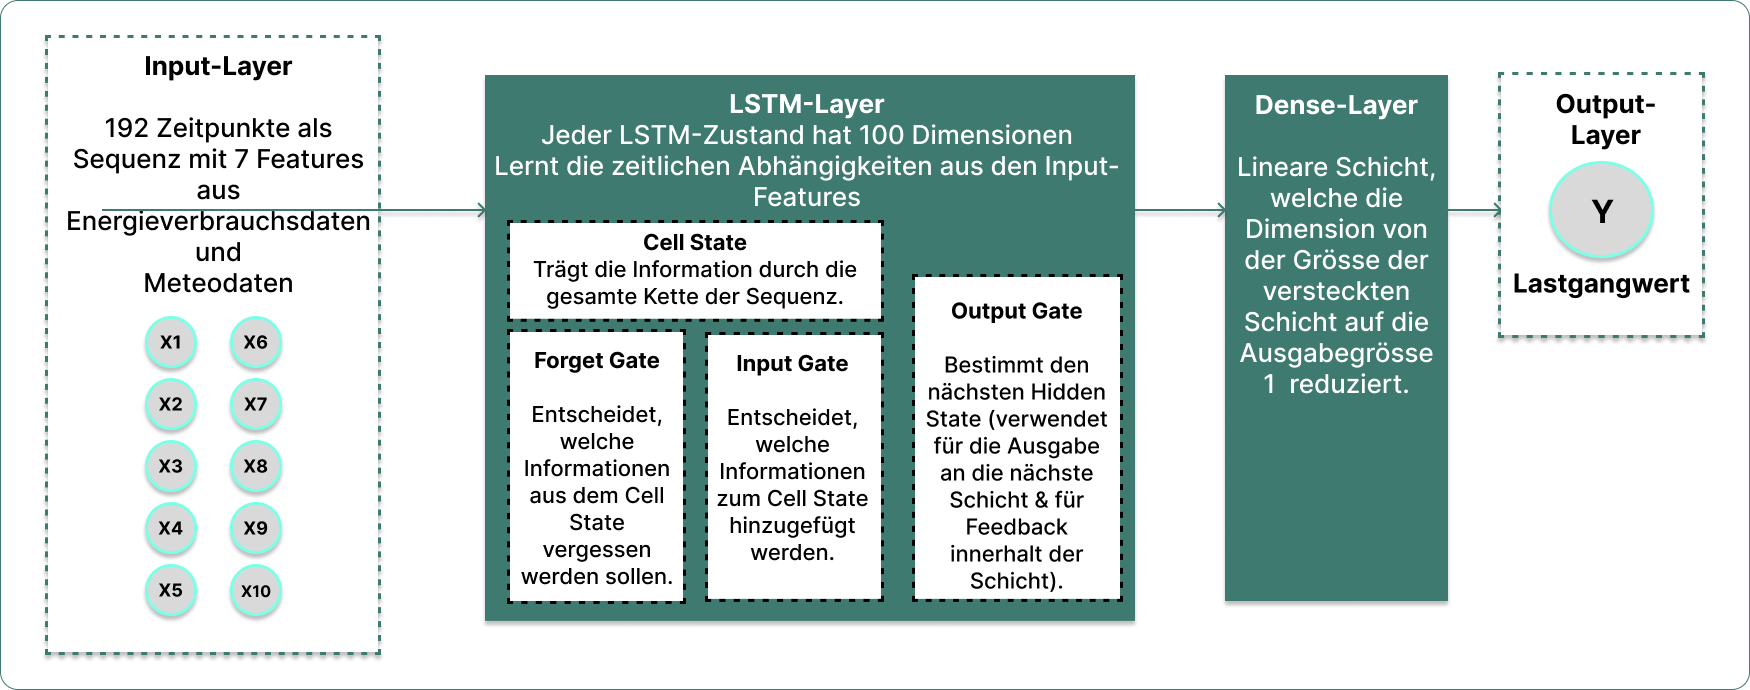
\includegraphics[width=15.25cm,keepaspectratio]{./images/Schematische_Darstellung_einer_LSTM_Arch.png}
\caption{Schematische Darstellung einer LSTM-Architektur zur Verarbeitung von Zeitreihendaten}
\small~\textit{(In Anlehnung an~\cite{LSTMArchitectureFigure} eigenerstellte Darstellung)}
\label{fig:schematische_darstellung_einer_lstm_architektur_zur_verarbeitung_von_zeitreihendaten}
\end{figure}
Die Abbildung \ref{fig:schematische_darstellung_einer_lstm_architektur_zur_verarbeitung_von_zeitreihendaten} illustriert \vref{subsubsec:long_short_term_memory_network__lstm_}eine schematische Darstellung einer \vref{subsubsec:long_short_term_memory_network__lstm_}LSTM-Architektur zur Verarbeitung von Zeitreihendaten. Die Eingabeschicht (Input-Layer) enthält die Eingabefeatures. In der vorliegenden Arbeit sind das 10 Variablen, die in Sequenzen von jeweils 192 Zeitpunkten an die LSTM-Layer übergeben werden. In der LSTM-Layer werden die Eingabedaten verarbeitet, um Langzeitabhängigkeiten in den Zeitreihendaten zu erkennen und relevante Informationen für die Vorhersage zu extrahieren. Der Zellzustand (Cell State) trägt relevante Information durch die Sequenz. Das Vergessensgitter (Forget Gate) entscheidet anhand einer Sigmoid-Aktivierungsfunktion, welche Informationen im Zellzustand vergessen und welche beibehalten werden sollen. Parallel dazu bewertet das Eingangsgitter (Input Gate) welche neuen Informationen zum Zellzustand hinzugefügt werden. Eine Sigmoid-Aktivierungsfunktion entscheidet, welche Werte aktualisiert werden und eine tanh-Schicht erzeugt neue Werte. Das Ausgangsgatter (Output Gate) verwendet die aktuelle Information des Zellzustands und den vorherigen verborgenen Zustand, um den nächsten verborgenen Zustand zu berechnen. Nach dem Durchlaufen der LSTM-Schicht gelangen die Daten in die lineare Schicht (Dense-Layer). Diese Schicht reduziert die Dimension der Daten von der Grösse der Hidden Layer auf die finale Ausgabegrösse. In der vorliegenden Studie erfolgt die Reduzierung von 100 auf die Ausgabegrösse 1, da das Ziel der Architektur die Vorhersage eines einzelnen Lastgangwertes pro Sequenz ist \cite{ChatGPTLSTMArchitecture}. Die Ergebnisse zu diesem Ansatz sind in \vref{subsubsec:lstm} dargestellt.


\subsubsection{Transformer}\label{subsubsec:transformer}
Das Konzept der Transformer-Modelle wurde erstmals in der Veröffentlichung \textit{Attention is All You Need} im Jahr 2017 vorgestellt \cite{PaperTransformerAttention} und wurde durch den Einsatz von Aufmerksamkeitsmechanismen bei der Verarbeitung natürlicher Sprache bekannt \cite{TowardsDataScienceTransformers}. Die Transformer-Architektur repräsentiert eine grundlegende Änderung von traditionellen sequenzbasierten Ansätzen wie LSTM oder herkömmlichen statistischen Methoden wie SARIMAX, Exponential Smoothing oder TBATS. Die Transformer-Architektur verarbeitet Sequenzen in einem Schritt und erfasst Beziehungen zwischen beliebigen Punkten einer Sequenz durch Mechanismen wie Selbst-Attention. Dadurch können komplexe Muster in den Daten oftmals besser erfasst und die Trainingszeiten verkürzt werden. Ein Transformer besteht aus den zwei Hauptkomponenten “{}Encoder”{} und “{}Decoder”{}, wobei in der Zeitreihenvorhersage meistens nur der Encoder-Teil verwendet wird. Dieser hat das Ziel, die nächsten Werte in der Sequenz vorherzusagen. Da die Architektur Sequenzen in einem Schritt erfasst, ist das Hinzufügen einer zusätzlichen Komponente bei Zeitreihendaten durch Positional Encoding ein wichtiger Schritt. Dadurch wird dem Modell ermöglicht, die Position der einzelnen Daten in der Sequenz zu verstehen und die Sequenz zu modellieren, auch wenn diese gleichzeitig verarbeitet werden \cite{ArticleTransformerforTimeSeriesModels}.


\begin{figure}[h]
\centering
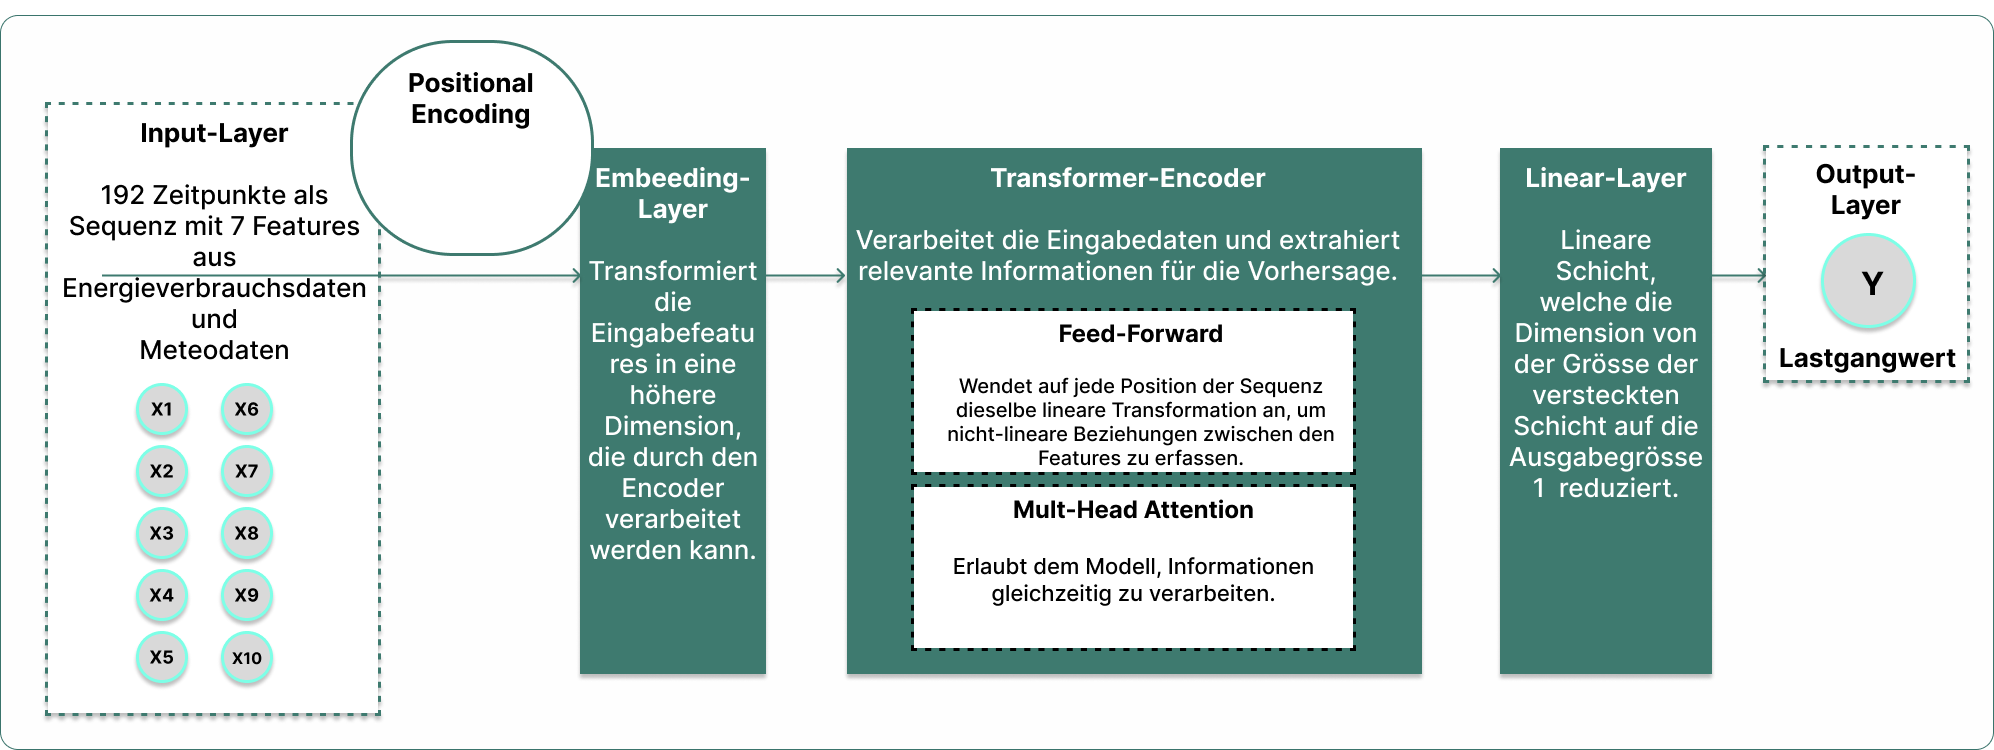
\includegraphics[width=15.25cm,keepaspectratio]{./images/Schematische_Darstellung_einer_Transform.png}
\caption{Schematische Darstellung einer Transformer-Architektur zur Verarbeitung von Zeitreihendaten}
\small~\textit{(In Anlehnung an~\cite{MediumTransformerArchitecture} eigenerstellte Darstellung)}
\label{fig:schematische_darstellung_einer_transformer_architektur_zur_verarbeitung_von_zeitreihendaten}
\end{figure}
Die Abbildung \ref{fig:schematische_darstellung_einer_transformer_architektur_zur_verarbeitung_von_zeitreihendaten} zeigt eine schematische Darstellung einer Transformer-Architektur zur Verarbeitung von Zeitreihendaten.  Die Eingabeschicht (Input-Layer) enthält die Eingabefeatures. In der vorliegenden Arbeit sind das 10 Variablen, die in Sequenzen von jeweils 192 Zeitpunkten an den Encoder übergeben werden. Das Positional Encoding wird jedem Eingabevektor zugefügt, um die Reihenfolge der Zeitpunkte in den nicht-rekurrenten Transformer-Strukturen zu erhalten. Die Einbettungsschicht (Embedding-Layer) transformiert die Eingabefeatures in eine höhere Dimension, damit der Encoder die Daten verarbeiten kann. Diese Schicht dient dazu, die Daten so umzuformen, damit sie für die Multi-Head-Attention-Mechanismen geeignet sind. Im Transformer-Encoder erfolgt die Extraktion und Verarbeitung der relevanten Informationen, damit das Modell eine Einsicht aus den Daten gewinnt. Die Multi-Head-Attention-Komponente wird verwendet, um gleichzeitig verschiedene Aspekte der Eingabedaten zu analysieren und Beziehungen zwischen allen Elementen einer Sequenz, unabhängig von deren Position, zu erkennen. Dies ermöglicht es dem Modell, komplexe Datenmuster effizient zu verarbeiten und wichtige Informationen aus den Daten hervorzuheben. Anschliessend verarbeitet die Feed-Forward-Methode jede Position der Sequenz unabhängig, indem sie eine Reihe von linearen Transformationen und nicht-linearen Aktivierungen anwendet. Diese Schicht transformiert die durch die Attention-Mechanismen angereicherten Daten, um die finale Ausgabe des Encoders vorzubereiten. Die Verwendung dieser beiden Mechanismen verbessert die Fähigkeit des Modells, sowohl die unmittelbare als auch die langfristige Relevant von Datenpunkten innerhalb der Sequenz zu erkennen. Nach der Verarbeitung durch den Encoder werden die Daten durch die lineare Schicht (Linear-Layer) geleitet. Diese Schicht reduziert die Dimension der Daten von der Grösse der versteckten Schicht auf die finale Ausgabegrösse. Schlussendlich wird der Ausgabewert ausgegeben. In der vorliegenden Studie erfolgt die Reduzierung von 100 auf die Ausgabegrösse 1, da das Ziel der Architektur die Vorhersage eines einzelnen Lastgangwertes pro Sequenz ist \cite{ChatGPTTransformerArchitecture}. Das \vref{subsubsec:transformer} präsentiert die Resultate zum Transformer-Modell. 


\subsection{Evaluation von Machine Learning-Modellen}\label{subsec:evaluation_von_machine_learning_modellen}
Das Ziel der Bewertung ist die Analyse, wie Vorhersagemodelle mit unbekannten Daten umgehen können \cite{ArticleEvaluationForecastingModel}. In der Trainingsphase lernen Modelle von einem Teil der Daten und werden in der Testphase mit unbekannten Daten getestet \cite{TowardsDataScienceTrainTest}. Um die Generalisierungsfähigkeit besser zu beurteilen, wird eine Validierungsphase mit externen Daten eingeführt. Beispielhaft umfasst diese Arbeit Trainingsdaten über den Zeitraum Januar 2021 bis Dezember 2023, abzüglich der letzten 48 Stunden, während die Testdaten aus den letzten 48 Stunden bestehen.


Die Bewertung und der Vergleich von Machine Learning-Modellen basieren auf verschiedenen Metriken \cite{BookTimeSeriesForecastingPython}. Die folgenden Fehlermetriken werden in dieser Arbeit verwendet: Der mittlere quadratische Fehler (MSE) misst die durchschnittliche quadratische Abweichung zwischen prognostizierten und tatsächlichen Werten, wobei grössere Fehler stärker gewichtet werden \cite{IBMForecastingStatistic}. Der mittlere absolute Fehler (MAE) berechnet den Durchschnitt der absoluten Differenzen zwischen den prognostizierten und den tatsächlichen Werten. Da der MAE alle Abweichungen gleich behandelt, ist er robust gegenüber Ausreissern \cite{IBMForecastingStatistic}. Die Quadratwurzel des MSE (RMSE), gibt Fehler in der Einheit der Zielvariable an - in dieser Arbeit ist die Einheit Kilowatt für die Zielvariable Lastgang \cite{IBMForecastingStatistic}. Der Mittlere absolute prozentuale Fehler (MAPE) gibt den Fehler zwischen Vorhersagen und tatsächlichen Werten in Prozent an. Diese Metrik ist besonders nützlich, um die Leistung von Modellen zu vergleichen, die unterschiedliche Skalen oder Einheiten haben \cite{IBMForecastingStatistic}. Generell lässt sich sagen, dass ein niedriger MAPE-Prozentfehler auf eine präzisere Vorhersage hindeutet. Eine mögliche Aufteilung zur Einschätzung ist, dass ein MAPE von weniger als 10 \% eine sehr präzise Vorhersage anzeigt, ein Wert zwischen 11 \% und 20~\% auf eine gute Vorhersage hindeutet, zwischen 21 \% und 50 \% als akzeptabel betrachtet wird und ein MAPE von über 51 \% eine ungenaue Vorhersage darstellt \cite{BookLewisForecastingMAPE}. Jedoch ist von der Autorin anzumerken, dass diese Einteilung mit Vorsicht zu geniessen ist und die Anforderung an die Vorhersagegenauigkeit sehr stark vom jeweiligen Thema abhängt. Das Bestimmtheitsmass \(R^{2}\) zwischen 0 und 1 gibt die erklärte Varianz der Zielvariable durch das Modell an. Dieses Mass wird für die Güte der Anpassung eines Regressionsmodells genutzt \cite{ScribbrLineareRegression}. Der Akaike Information Criterion (AIC) ist ein Mass zur Bewertung verschiedener statistischer Modelle unter Berücksichtigung ihrer Komplexität. Das AIC belohnt die Anpassungsgüte des Modells, bestraft jedoch gleichzeitig die Modelle mit einer höheren Anzahl an Parametern. Ein niedriger AIC weist auf ein besseres Modell hin \cite{ModelSelectionAICBIC}. Der Bayesian Information Criterion (BIC) bewertet die Qualität von Modellen ähnlich wie der AIC unter Berücksichtigung ihrer Komplexität, ist im Vergleich zum AIC jedoch strenger hinsichtlich der Bestrafung für die Anzahl der Modellparameter \cite{ModelSelectionAICBIC}.


\newpage
\section{Ergebnisse}\label{sec:ergebnisse}
In diesem Kapitel werden die Ergebnisse präsentiert. \vref{subsec:explorative_datenanalyse__eda_} stellt die explorative Datenanalyse (EDA) zu den Energieverbrauchsdaten aus den sieben Trafostationen vor. Zudem werden der Datensatz der Meteodaten sowie eine Korrelationsanalyse zwischen den beiden verwendeten Datensätzen präsentiert. Das \vref{subsec:anwendung_der_machine_learning_modelle} fasst die Ergebnisse der angewendeten Modelle zusammen. Dabei werden für jedes Modell die Modellarchitektur, spezifische Vorverarbeitungsschritte, die Trainings- und Testprozesse sowie die Fehlermetriken und die vorhergesagten Werte über 48 Stunden vorgestellt. Im letzten \vref{subsec:evaluation_und_vergleich_der_machine_learning_modelle} werden die Machine Learning-Modelle evaluiert und nach definierten Kriterien bewertet.

\subsection{Explorative Datenanalyse (EDA)}\label{subsec:explorative_datenanalyse__eda_}
Die EDA trug dazu bei, ein besseres Verständnis über die verwendeten Zeitreihendaten zu erlangen, relevante Variablen für die Modelle zu identifizieren und die Parameter der jeweiligen Modelle zu bestimmen.

\subsubsection{Energieverbrauchsdaten im 15-Minuten Intervall 2021 bis 2023}\label{subsubsec:energieverbrauchsdaten_im_15_minuten_intervall_2021_bis_2023}
Der Datensatz der Energieverbrauchsdaten besteht aus der Spalte 'Timestamp', welche den Zeitstempel in einem standardisierten Format 'YYYY-MM-DD HH:MM:SS' zeigt und aus der Spalte Lastgang, die den Energieverbrauchswert in Kilowatt zeigt. Für die Datenbereinigung wurden im Datensatz Ergebniszeilen aus den Daten entfernt. Zudem war der Mitternachtszeitstempel in den Daten, die aus einem SAP-System stammen, als Hashtag '\#' gespeichert. Dieser Zeitstempel wurde in 00:00:00 umgewandelt. Für die EDA wurden die Daten auf fehlende Werte überprüft. Es hat sich gezeigt, dass keine NaN-Werte vorliegen, aber 12 Zeitstempel vollständig fehlen. Für den Zeitraum von drei Jahren müssten 105'120 Datenzeilen vorliegen, da pro Tag 96 Datenzeilen entstehen. Aufgrund der Zeitverschiebung fehlen in jedem Jahr vier Datenzeilen. Diese wurden anhand der 'fillna()'-Methode mit dem nächsten gültigen Wert in der Zeitreihe aufgefüllt. Dies ist insbesondere ein wichtiger Schritt im Hinblick auf die kombinierte Nutzung mit dem Datensatz der Meteodaten, bei dem diese 12 Zeitstempel nicht fehlen. 

Um mit dem Datensatz weiterzuarbeiten, wurde die Spalte Lastgang in einen numerischen Datentyp umgewandelt. Weiter wurden Kennzahlen wie der Mittelwert und die Quartile anhand der deskriptiven Statistik ausgegeben, die in Abbildung \ref{fig:desktriptive_statistik_der_variable_lastgang_in_kilowatt} dargelegt werden. Der Mittelwert des Energieverbrauchs aus den 7 Trafostationen liegt bei 676.31 kW, während der Median bei 634.75 kW liegt. Der geringste Energieverbrauch liegt bei 50.54 kW, während der höchste Verbrauch bei 1519.67 kW liegt. Die Quartile zeigen, dass  25~\% der Daten unter 509.35 kW, 50 \% unter 634.75 kW und 75 \% der Daten unter 824.92 kW liegen. Die Standardabweichung beträgt 219.77 kW, was eine durchschnittliche Abweichung der Verbrauchswerte vom Mittelwert darstellt. Indem die Standardabweichung durch den Mittelwert dividiert wird, ergibt sich ein Variationskoeffizient von 32.5 \% \cite{VariationskoeffizientStudyflix}.


\begin{figure}[h]
\centering
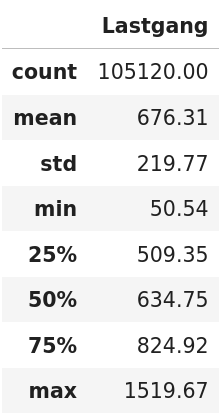
\includegraphics[width=3.25cm,keepaspectratio]{./images/Desktriptive_Statistik_der_Variable_Last.png}
\caption{Desktriptive Statistik der Variable Lastgang in Kilowatt}
\small~\textit{(Quelle: Eigene Darstellung).}
\label{fig:desktriptive_statistik_der_variable_lastgang_in_kilowatt}
\end{figure}
Nach der ersten Analyse der Daten wurden Visualisierungen des Datensatzes erstellt. Das Histogramm \ref{fig:histogramm_fuer_die_15_minuten_intervalle_der_variable_lastgang} veranschaulicht, dass die Energieverbrauchsdaten, gemessen in 15-Minuten-Intervallen, normalverteilt sind und einen Modus mit einer deutlichen Spitze aufweisen. Der Grossteil der Daten konzentriert sich um den Gipfel herum, woraus sich schliessen lässt, dass der Energieverbrauch häufig zwischen den Werten 450 kW und 650 kW liegt. Die Schiefe, erkennbar an einem längeren Schwanz in Richtung höherer Werte, verdeutlicht, dass der Energieverbrauch zu bestimmten Zeitpunkten signifikant über dem Durchschnitt liegt. Der flache Bereich an den Enden bedeutet, dass es nur wenige sehr niedrige und sehr hohe Verbrauchswerte gibt. Die dunklere Linie zeigt die geglättete Version des Histogramms.


\begin{figure}[h]
\centering
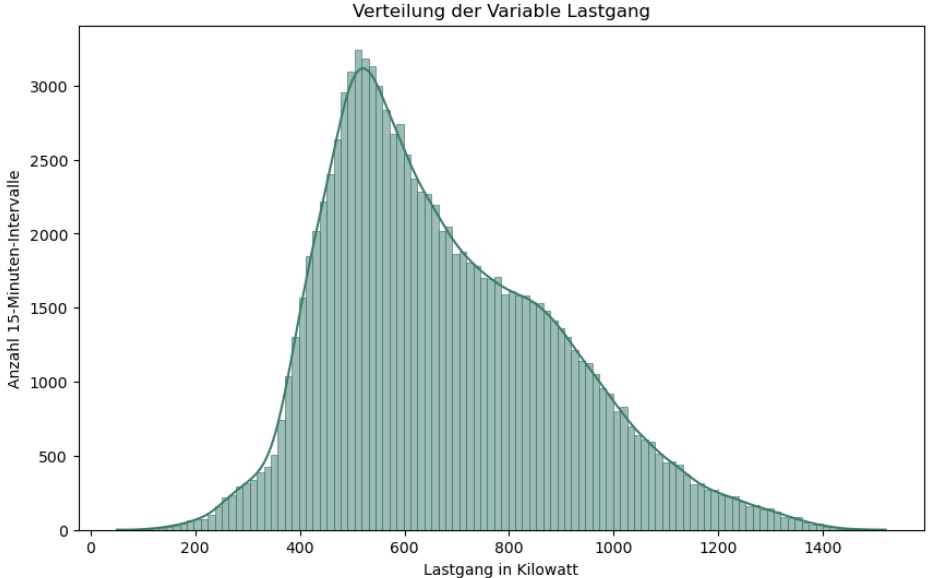
\includegraphics[width=11.75cm,keepaspectratio]{./images/Histogramm_fuer_die_15_Minuten_Intervall.png}
\caption{Histogramm für die 15-Minuten-Intervalle der Variable Lastgang}
\small~\textit{(Quelle: Eigene Darstellung).}
\label{fig:histogramm_fuer_die_15_minuten_intervalle_der_variable_lastgang}
\end{figure}
Der Box-Plot in Abbildung \ref{fig:boxplot_der_lastgang_daten_mit_median__quartilsbereichen_und_whiskers} zeigt Ausreisser des Datensatzes sowie den Median. Die Whiskers markieren Werte innerhalb von 1.5*IQR um das untere und obere Quartil. Alle Werte ausserhalb gelten als Ausreisser. Diese beeinflussen den Mittelwert und die Varianz stark, während der Median unbeeinflusst ist.


\begin{figure}[h]
\centering
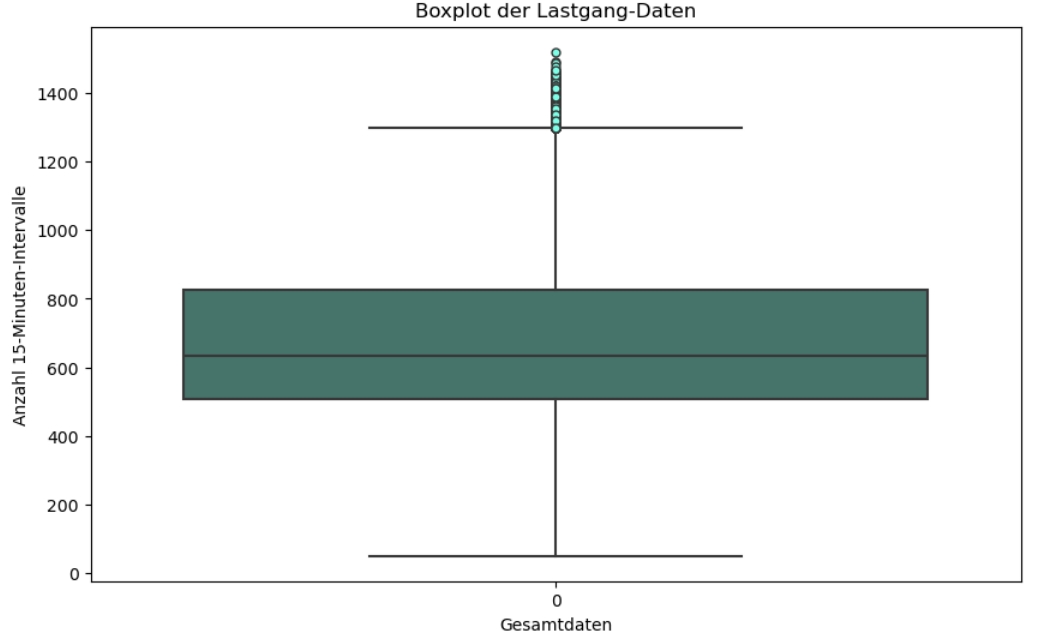
\includegraphics[width=11.75cm,keepaspectratio]{./images/Boxplot_der_Lastgang_Daten_mit_Median__Q.png}
\caption{Boxplot der Lastgang-Daten mit Median, Quartilsbereichen und Whiskers}
\small~\textit{(Quelle: Eigene Darstellung).}
\label{fig:boxplot_der_lastgang_daten_mit_median__quartilsbereichen_und_whiskers}
\end{figure}
Um die Zeitreihe zu visualisieren, wurde ein Zeitreihendiagramm erstellt. Die Abbildung \ref{fig:15_minuten_intervall_der_lastgang_daten__kw__ueber_den_zeitraum_2021___2023_mit_dem_mittelwert} zeigt die Zeitreihe des Energieverbrauchs in Kilowatt für jedes 15-Minuten-Intervall über den Zeitraum Januar 2021 bis Dezember 2023. Das Diagramm macht bereits die jährliche Saisonalität im Lastgang klar erkennbar, wobei in den Sommermonaten der Energieverbrauch tiefer ist als über die Wintermonate.


\begin{figure}[h]
\centering
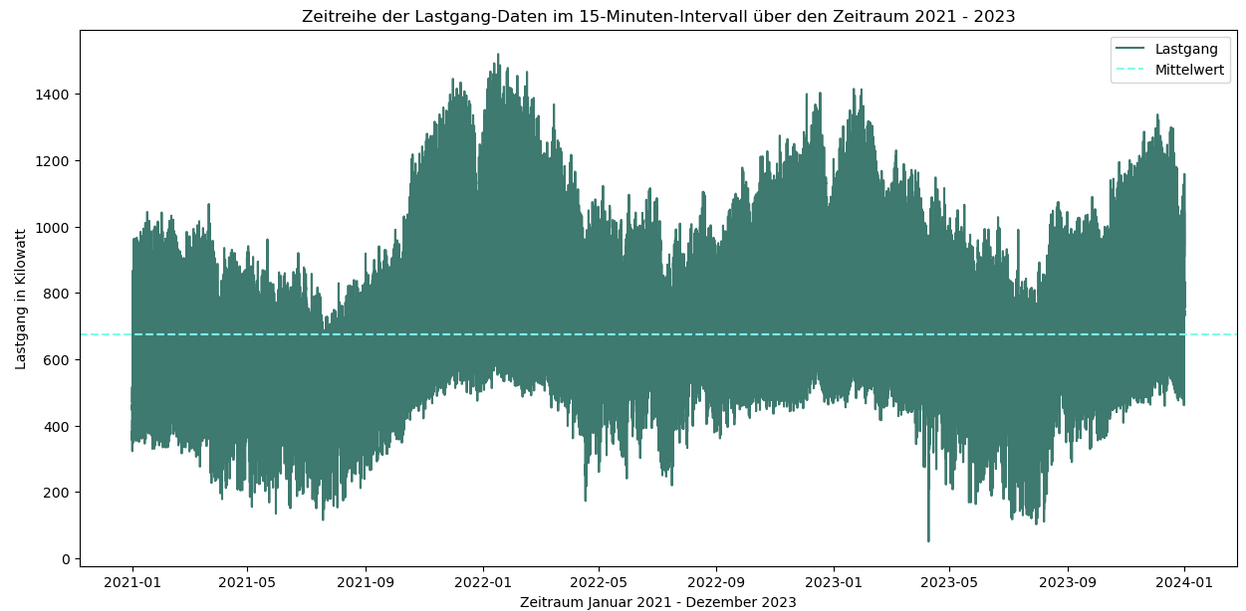
\includegraphics[width=11.75cm,keepaspectratio]{./images/15_Minuten_Intervall_der_Lastgang_Daten_.png}
\caption{15-Minuten-Intervall der Lastgang-Daten (kW) über den Zeitraum 2021 - 2023 mit dem Mittelwert}
\small~\textit{(Quelle: Eigene Darstellung).}
\label{fig:15_minuten_intervall_der_lastgang_daten__kw__ueber_den_zeitraum_2021___2023_mit_dem_mittelwert}
\end{figure}
Spezifisch für die Zeitserienanalyse wurde in einem nächsten Schritt das Muster der Zeitreihendaten auf verschiedenen Zeitebenen untersucht, um die Trends und periodischen Muster in den Daten noch detaillierter zu erkennen. Der Datensatz wurde hierbei auf tägliche, wöchentliche und monatliche Basis aggregiert. Die Plots in Abbildung \ref{fig:aggregierte_zeitreihen_der_lastgang_daten__taeglich__woechentlich__monatlich_} zeigen die durchschnittlichen Lastgangwerte. Der erste Plot stellt die täglichen Schwankungen dar, während beim zweiten Plot, wöchentlicher Mittelwert, die täglichen Schwankungen geglättet sind. In diesem zweiten Plot lässt sich der Trend über die Wochen klarer erkennen. Zu bestimmten Zeiten des Jahres zeigt der Mittelwert eine stärkere Variabilität auf, was auf wöchentliche Muster hindeuten kann. Der letzte Plot visualisiert die monatlichen Mittelwerte, wodurch der langfristige Trend ersichtlich wird. Es ist erkennbar, dass der Lastgang in bestimmten Monaten höher ist, was auf saisonale Faktoren oder Feiertage hinweisen kann.


\begin{figure}[h!]
\centering
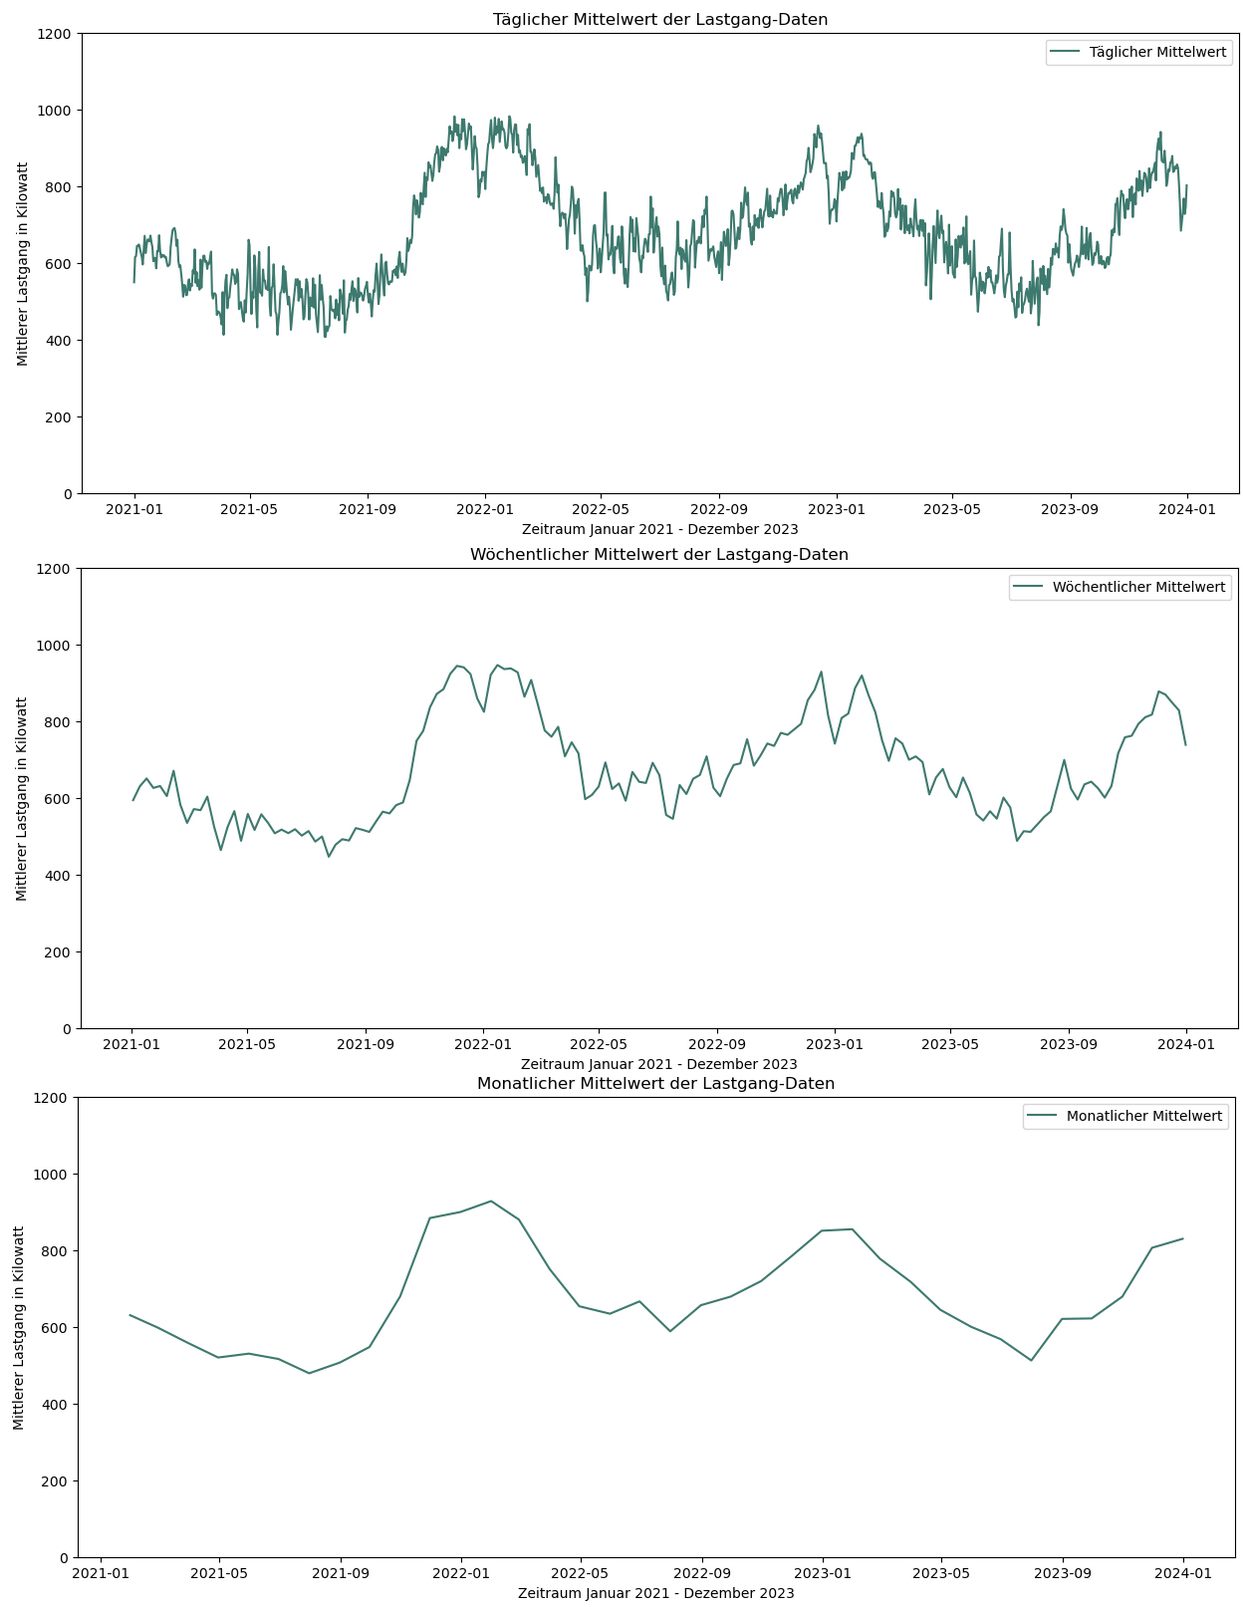
\includegraphics[width=11.75cm,keepaspectratio]{./images/Aggregierte_Zeitreihen_der_Lastgang_Date.png}
\caption{Aggregierte Zeitreihen der Lastgang-Daten (täglich, wöchentlich, monatlich)}
\small~\textit{(Quelle: Eigene Darstellung).}
\label{fig:aggregierte_zeitreihen_der_lastgang_daten__taeglich__woechentlich__monatlich_}
\end{figure}
Da das Ziel dieser Arbeit war, Vorhersagen für den Zeitraum von 48 Stunden zu generieren, wurden die Plots für zwei Wochentage im Sommer wie im Winter ausgegeben. Die Abbildung \ref{fig:lastgang_in_kilowatt_ueber_den_zeitraum_von_48_stunden_im_sommer_und_winter} zeigt den Energieverbrauch an einem Donnerstag und einem Freitag im Juni respektive im Dezember. Deutlich erkennbar sind die Spitzen, die während den Abendstunden generiert werden, wobei der Energieverbrauch an einem Wintertag deutlich höher ausfällt.


\begin{figure}[h!]
\centering
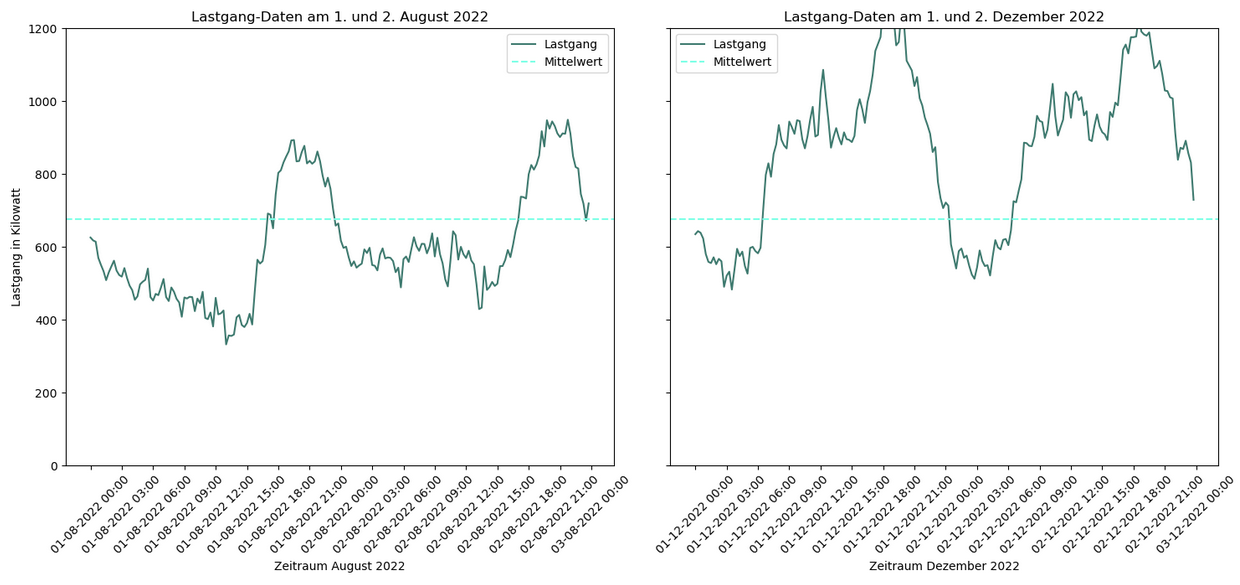
\includegraphics[width=11.75cm,keepaspectratio]{./images/Lastgang_in_Kilowatt_ueber_den_Zeitraum_.png}
\caption{Lastgang in Kilowatt über den Zeitraum von 48 Stunden im Sommer und Winter}
\small~\textit{(Quelle: Eigene Darstellung).}
\label{fig:lastgang_in_kilowatt_ueber_den_zeitraum_von_48_stunden_im_sommer_und_winter}
\end{figure}
Als nächstes zeigt die Abbildung \ref{fig:autokorrelation_der_lastgang_werte_zu_verschiedenen_zeitverzoegerungen} das Autokorrelationsdiagramm für die Lastgangdaten. Damit wurde überprüft, wie die Lastgangwerte mit sich selbst zu verschiedenen Zeitverzögerungen korrelieren. In der Zeitreihenanalyse ist dies ein wichtiges Instrument, um zu verstehen, ob es im Laufe der Zeit wiederkehrende Muster gibt und um die Parameter für die Modellanwendungen, insbesondere SARIMAX-Modelle, zu definieren \cite{NeptuneAutocorrelationSARIMA}. Die Grafik veranschaulicht die Autokorrelation der Zeitreihe Lastgang für verschiedene Verzögerungen, sogenannte Lags. Die Autokorrelation misst die lineare Beziehung zwischen zeitlich versetzten Werten derselben Zeitreihe \cite{NeptuneAutocorrelationSARIMA}. Zu Beginn, bei geringen Lags, ist die Autokorrelation hoch und positiv. Das deutet darauf hin, dass aufeinanderfolgende Messungen stark miteinander korrelieren, was wiederum bedeutet, dass Werte in benachbarten Zeitreihendaten ähnlich sind. Dieses Muster ist bei Energieverbrauchsdaten zu erwarten, da im Verbrauch innerhalb einzelner Stunden typischerweise keine extremen Schwankungen vorliegen. Anschliessend lässt sich ein wellenförmiges Muster mit regelmässigen Spitzen und Senken erkennen, das auf eine saisonale Komponente im Datensatz hindeutet. Diese Beobachtung bestätigt die saisonalen Schwankungen zwischen den Sommer- und Wintermonaten, die bereits in den Zeitreihendiagrammen ersichtlich waren. Die Stärke der Autokorrelation nimmt mit zunehmendem Lag, mit zunehmender Verzögerung, ab. Das heisst, dass die Ähnlichkeit zwischen den Datenpunkten abnimmt, je weiter sie zeitlich auseinander liegen. An einigen Stellen fällt die Autokorrelation unter null. Dies bedeutet, dass die Werte in der Zeitreihe zu bestimmten Verzögerungen negativ korreliert sind. Konkret auf die Lastgangdaten bezogen bedeutet dies, dass wenn die Verbrauchswerte zu einem gegebenen Zeitpunkt ihren Durchschnittswert überschreiten, sie nach einem bestimmten Zeitintervall wahrscheinlich darunter liegen werden. Dies gilt ebenso für den umgekehrten Fall, wenn die Verbrauchswerte zu einem gegebenen Zeitpunkt ihren Durchschnittswert unterschreiten. Ein einfaches Beispiel dafür ist, dass nach einer Periode hoher Verbrauchsnachfrage in den frühen Abendstunden eine Periode niedriger Nachfrage in der Nacht folgt.

\begin{figure}[h!]
\centering
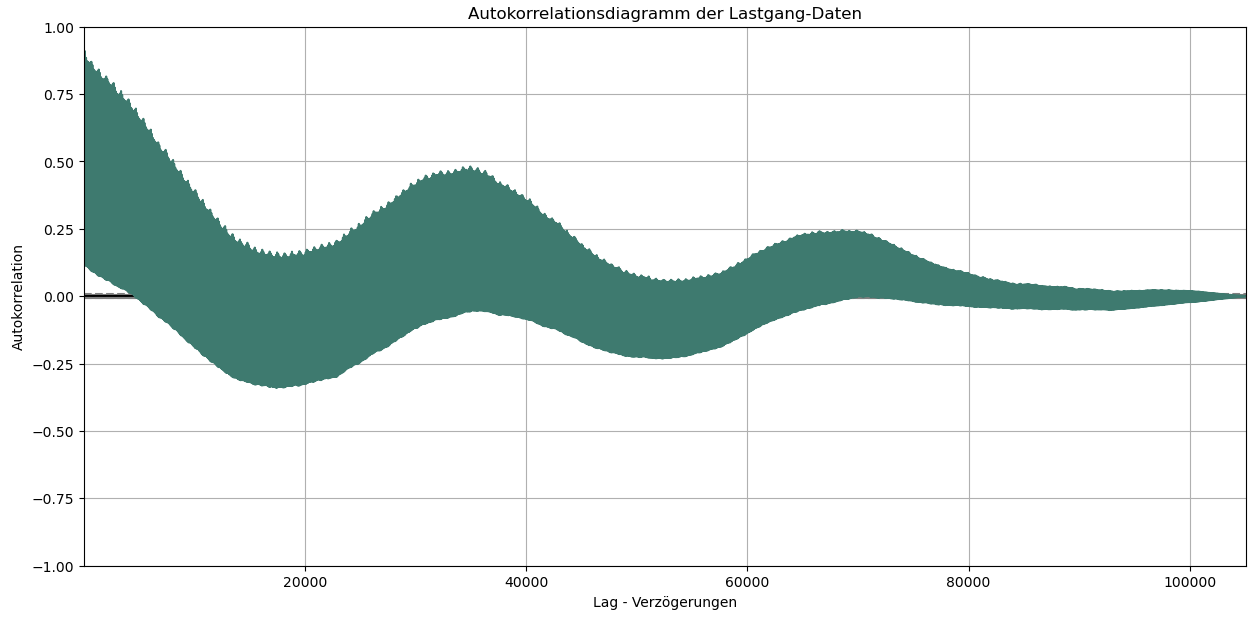
\includegraphics[width=11.75cm,keepaspectratio]{./images/Autokorrelation_der_Lastgang_Werte_zu_ve.png}
\caption{Autokorrelation der Lastgang-Werte zu verschiedenen Zeitverzögerungen}
\small~\textit{(Quelle: Eigene Darstellung).}
\label{fig:autokorrelation_der_lastgang_werte_zu_verschiedenen_zeitverzoegerungen}
\end{figure}
Im nächsten Schritt wurde eine Dekomposition der Zeitreihe durchgeführt. Die Analyse der Zeitreihenkomposition zerlegt eine Zeitreihe in ihre Hauptkomponenten Trend, Saisonalität und Residuen und gibt diese drei Komponenten als einzelne Plots aus. Dadurch wurden die saisonalen Effekte erkenntlich, was wiederum für die anschliessende Modellierung wichtig war. Die Abbildung \ref{fig:dekomposition_der_zeitreihe_mit_trend__saisonalitaet_und_residuen} zur Dekomposition ist in \vref{sec:zusaetzliche_grafiken_aus_der_exploratorischen_datenanalyse__eda_} zu finden.


Im letzten Schritt der EDA wurde ein Stationaritätstest anhand des Augmented-Dickey-Fuller-Test (ADF-Test) durchgeführt. Dieser Test überprüft, ob das Datenset stationär ist. Die Durchführung des Stationaritätstest war wichtig, da einige Modelle wie beispielsweise SARIMAX eine Stationarität der Daten erwartet. Stationarität bedeutet, dass die statistischen Eigenschaften der Zeitreihe wie Mittelwert, Varianz und Autokorrelation im Laufe der Zeit konstant bleiben \cite{StationaryDatacamp}. Die ADF-Teststatistik hat einen Wert von -18.34 und ein p-Wert von praktisch 0 ergeben. Dieses Resultat steht für eine starke Evidenz gegen die Nullhypothese (H0). Es kann daher davon ausgegangen werden, dass die Zeitreihe der Energieverbrauchsdaten stationär ist und somit konstante statistische Eigenschaften über die Zeit hat.

\subsubsection{Meteodaten im 15-Minuten-Intervall 2021 bis 2023}\label{subsubsec:meteodaten_im_15_minuten_intervall_2021_bis_2023}
Der Originaldatensatz der Meteodaten besteht aus den Zeitinformationen wie Monat, Tag des Monats, Tag des Jahres, Stunde und Minuten sowie 13 Variablen. In einem ersten Schritt wurden die Zeitinformationen zu einem Zeitstempel in einem standardisierten Format 'YYYY-MM-DD HH:MM:SS' zusammengesetzt und somit an den Datensatz der Energieverbrauchsdaten angepasst. Auch wurden die Namen der Variablen in verständlichere Bezeichnungen geändert. In einem zweiten Schritt wurde der Datensatz auf das Fehlen von Werten untersucht, wobei keine fehlenden Werte festgestellt werden konnten.

Für den weiteren Einsatz wurde der Datensatz mit den Variablen verwendet, die in Tabelle \ref{tab:VariablenMeteodatensatz} aufgeführt sind. Diese Tabelle listet auch die Korrelationen zwischen den unabhängigen und der abhängigen Variable 'Lastgang' auf. Die Ergebnisse der Korrelationsanalyse zeigen relativ schwache bis mässige Korrelationen. Alle Korrelationen liegen zwischen -0.4 und 0.4. Die Variable 'StundenwertStrahlung' weist mit -0.383 die stärkste negative Korrelation auf, gefolgt von 'Globalstrahlung\_15Min' und 'StrahlungGeneigteFläche' (beide -0.381), 'TheorPVProd' (-0.373), 'Direktnormalstrahlung' (-0.334), 'Lufttemperatur' (-0.332), und 'Schönwetterstrahlung' (-0.31). Schwächere negative Korrelationen als -0.3 wurden in nachfolgenden Modellen nicht berücksichtigt. Bei negativ korrelierten Variablen bedeutet ein Anstieg der Variable einen Rückgang des Lastgangwerts. Die negativen Korrelationen scheinen darauf hinzudeuten, dass an sonnenreichen Tagen ein geringerer Energiebedarf mit gleichzeitiger höherer Energieproduktion durch Photovoltaikanlagen besteht. Weitere Ausführungen dazu sind in \vref{subsec:zusammenfassung_und_bewertung_der_forschungsergebnisse} zu finden. 'Windgeschwindigkeit' ist die einzige Variable, die mit 0.11 eine schwache positive Korrelation aufweist. Das bedeutet, dass ein Anstieg der Windgeschwindigkeit zu einem Anstieg des Lastgangwerts führt.


\begin{landscape}~


\begin{center}
\footnotesize
\begin{longtable}{|p{15.3cm}|p{4.4cm}|p{1.7cm}|}
\hline
\textbf{Variablenname und Bedeutung der Variable} & \textbf{Einheit der Variable} & \textbf{Korrelation} \\
\hline
StundenwertStrahlung: Menge der Solarstrahlung innerhalb einer Stunde. & Watt pro Quadratmeter (W/m²) & -0.382996 \\
\hline
Globalstrahlung15Min: Gesamtmenge an Sonnenenergie, die pro Quadratmeter auf die Erdoberfläche trifft. & Watt pro Quadratmeter (W/m2) & -0.381206 \\
\hline
StrahlungGeneigteFläche: Solarstrahlung, die auf eine geneigte Fläche trifft. Wird nicht weiter berücksichtigt, da beim Zusammenstellen der Daten keine Neigung eingestellt wurde, wodurch der Wert der horizontalen Einstrahlung entspricht. & - & -0.381206 \\
\hline
TheorPVProd: Die Menge an Strom, die von einer Photovoltaikanlage mit einer Leistung von 1 Kilowatt unter idealen Bedingungen produziert wird. & Kilowattstunden (kWh) & -0.373244 \\
\hline
Direktnormalstrahlung: Direkte Solarstrahlung, die nicht durch atmosphärische Streuung oder Reflexion beeinflusst wurde. & Watt pro Quadratmeter (W/m²) & -0.333582 \\
\hline
Lufttemperatur: Temperatur der Luft. & Grad Celsius (°C) & -0.331660 \\
\hline
Schönwetterstrahlung: Die Globalstrahlung, die man bei klarem Himmel erhalten würde. & Watt pro Quadratmeter (W/m²) & -0.309564 \\
\hline
ExtraterrestrischeStrahlung: Menge der Sonnenstrahlung ausserhalb der Erdatmosphäre. & Watt pro Quadratmeter (W/m²) & -0.298291 \\
\hline
Taupunkttemperatur: Die Temperatur, bei der Luft mit der aktuellen Feuchtigkeit gesättigt ist und Kondensation beginnt. & Grad Celsius (°C) & -0.290874 \\
\hline
Diffusstrahlung: Anteil der Solarstrahlung, der nach der Streuung durch die Atmosphäre die Erdoberfläche erreicht. & Watt pro Quadratmeter (W/m²) & -0.239543 \\
\hline
DiffusstrahlungGeneigteFläche: Diffuse Solarstrahlung, die auf eine geneigte Fläche trifft. Relevant für die Berechnung der Solarleistung auf schrägen Oberflächen. & Watt pro Quadratmeter (W/m²) & -0.239543 \\
\hline
Sonnenhöhe: Der Winkel der Sonne über dem Horizont an einem bestimmten Standort und Zeitpunkt. & Grad (°) & -0.175188 \\
\hline
Windgeschwindigkeit: Die Geschwindigkeit des Windes. & Meter pro Sekunde (m/s) & 0.109349 \\
\hline
TimestampWeather: Zusammengesetzter Zeitstempel aus den Zeitinformationen Monat, Tag des Monats, Tag des Jahres, Stunde und Minuten. & YYYY-MM-DD HH:MM:SS & - \\
\hline
dy: Tag des Jahres. & Zahl 0-365 & - \\
\hline
\caption{Variablen des Meteodatensatzes, ihre Bedeutung und die jeweilige Korrelation zur Variable Lastgang - sortiert in absteigender Form.}
\label{tab:VariablenMeteodatensatz}\\
\end{longtable}
\end{center}\end{landscape}~

\subsection{Anwendung der Machine Learning-Modelle}\label{subsec:anwendung_der_machine_learning_modelle}
Dieses Kapitel präsentiert die Ergebnisse der traditionellen Machine Learning-Methoden wie Regressionsanalyse, SARIMAX, Exponential Smoothing und TBATS sowie der \mbox{Deep} Learning wie LSTM und Transformer-Architekturen, die auf die Energieverbrauchsdaten angewendet wurden.


Für die Modellberechnungen standen Ressourcen einer Ubuntu-basierten Maschine mit einem AMD EPYC 7313P 16-Core Prozessor, 146 GB Arbeitsspeicher und zwei NVIDIA A100 80GB PCIe Grafikkarten zur Verfügung, die jeweils mit der neuesten CUDA-Version 12.4 betrieben werden \cite{ChatGPTRessourcenML}. Zwei separate Python-Conda-Umgebungen wurden für die Anwendung der statistischen Methoden und der Deep Learning-Methoden erstellt, um Abhängigkeiten zwischen den Python-Paketen zu reduzieren. Die für die Modelle erforderlichen Pakete und Bibliotheken können unter den angegebenen Links im Anhang in \vref{sec:quellcode_der_machine_learning__und_deep_learning_modelle} eingesehen werden.


Bei allen Methoden wurde in einem ersten Schritt die Energieverbrauchsdaten aus dem Zeitraum Januar 2021 bis Dezember 2023 aus verschiedenen Dateien eingelesen, zu einem Datenrahmen 'dfEnergyAll' zusammengeführt und basierend auf dem Zeitstempel gruppiert. Bei der linearen Regression, SARIMAX sowie bei den LSTM- und Transformer-Architekturen wurden zusätzlich die Meteodaten aus demselben Zeitraum eingelesen und zu einem Datenrahmen 'dfClimaAll' zusammengeführt. Durch das Setzen des Zeitstempels als Index wurde das Berechnen gleitender Durchschnitte vereinfacht und eine chronologische Ordnung der Daten sichergestellt. Bei den Modellen, die externe Variablen zulassen, wurden anschliessend die Spalten aus dem 'dfClimaAll'-Datenrahmen sowie die beiden zusätzlich erstellten Variablen 'Lastgang\_Moving\_Average' und 'Lastgang\_First\_Difference' zum Datenrahmen 'dfEnergyAll' hinzugefügt. Diese beiden Variablen wurden zur Glättung kurzfristiger Fluktuationen und zur Berechnung der Differenzen zwischen aufeinanderfolgenden Werten erstellt. Aus dem Meteodatensatz wurden als erklärende Variablen diejenigen Variablen hinzugefügt, die mit dem Energieverbrauch eine höhere Korrelation als +-0.3 aufweisen. Die Korrelationen sind in der Tabelle Referenz aus dem \vref{subsec:explorative_datenanalyse__eda_} zu entnehmen. Die Aufteilung der Daten in Trainings- und Testdatensätze erfolgte für alle Modelle gleich: Daten bis auf die letzten 48 Stunden bildeten den Trainingsdatensatz, während die letzten 192 Datenpunkte als Testdatensatz dienten. 192 Datenpunkte setzen sich aus vier Intervallen pro Stunde über 48 Stunden zusammen.

Die angegebenen Zahlen dieser Arbeit sind auf zwei Nachkommastellen gerundet. Im Rahmen dieser Arbeit gilt ein Prognosemodell als angemessen leistungsfähig, wenn es in der Lage ist, Energieverbrauchsdaten in 15-Minuten-Intervallen über einen Zeitraum von 48 Stunden mit einem Mean Absolute Percentage Error (MAPE) von unter 10 \% vorherzusagen.

\subsubsection{Lineare Regression}\label{subsubsec:lineare_regression}
Die Lineare Regression diente als Vergleichsgrundlage, um die Leistung der nachfolgenden komplexeren Modelle daran zu messen. Dieser Ansatz wurde gewählt, da dies gängige Praxis in der Forschung ist, wie aus der Forschungsliteratur aus \vref{subsec:verwandte_arbeiten} zu entnehmen ist. 

Nach den Vorverarbeitungsschritten, die in \vref{subsec:anwendung_der_machine_learning_modelle} vorgestellt sind, wurden die Daten auf Werte zwischen 0 und 1 skaliert. Für die Modellanwendung wurden die Daten zunächst in Trainings- und Testdaten unterteilt. Anschliessend wurde die Zielvariable 'Lastgang' und die verschiedenen erklärenden Variablen definiert. Das Modell wurde anhand den Trainingsdaten erstellt und angepasst. Schlussendlich folgte die Vorhersage der Testdaten über 48 Stunden hinweg.

Die Modellzusammenfassung weist ein \(R^{2}\)-Wert von 0.46 aus. Dies bedeutet, dass ungefähr 46 \% der Varianz in den tatsächlichen Lastgangwerten durch das Modell erklärt werden. Dieses Resultat deutet auf eine moderate Modellanpassung hin. Das Modell zeigt aber mit einem p-Wert von 0.00, dass eine signifikante Korrelation zwischen den vorhergesagten und den tatsächlichen Werten vorliegt. Das bedeutet, dass das Modell eine bessere Anpassung liefert, als erwartet werden würde, wenn es keine Beziehung zwischen den unabhängigen Variablen und der abhängigen Variable 'Lastgang' gäbe. Die Koeffizienten des Regressionsmodells legen weitere Einblicke in die Beziehung zwischen den erklärenden Variablen und dem Lastgang dar. Die Variable 'Lastgang\_Moving\_Average'   hat mit einem Koeffizienten von 0.41 den stärksten positiven Einfluss auf die Zielvariable 'Lastgang'. Dieser Wert deutet auf die Bedeutung von zeitlichen Trends im Energieverbrauch hin. Die Variablen 'Globalstrahlung\_15Min', 'StrahlungGeneigteFläche' sowie 'StundenwertStrahlung' weisen negative Koeffizienten auf, was auf eine inverse Beziehung zu den Lastgangwerten hinweist.


Die Fehlermetriken des Modells weisen einen MSE von 29459.06 \(kW^{2}\), einen MAE von 144.13 kW und einen RMSE von 171.64 kW auf. Diese Werte sind in absoluten Begriffen relativ hoch. Dies deutet darauf hin, dass die Vorhersagen des Modells eine gewisse Unsicherheit aufweisen. Insbesondere der RMSE, welcher grössere Abweichungen stärker gewichtet, zeigt, dass das Modell Schwierigkeiten hat, einige Spitzenwerte genau vorherzusagen. Der MAPE von 19.29 \% deutet darauf hin, dass die Vorhersagen des Modells im Durchschnitt um etwa ein Fünftel vom tatsächlichen Wert abweichen. Die Analyse der Modellanpassung ergibt AIC- und BIC-Werte von jeweils -1.656e+05.


Wie aus der Abbildung \ref{fig:lineare_regression_ueber_48_stunden_mit_energieverbrauchsdaten_und_meteodaten_als_input} zu entnehmen ist, bestätigt der Plot diese Ergebnisse. In den tatsächlichen Lastgangwerten sind die typischen Täler und Spitzen wie beispielsweise in den Abendstunden erkennbar, während sich die vorhergesagten Werte um den Mittelwert von 676.31 kW herum bewegen.


\begin{figure}[h!]
\centering
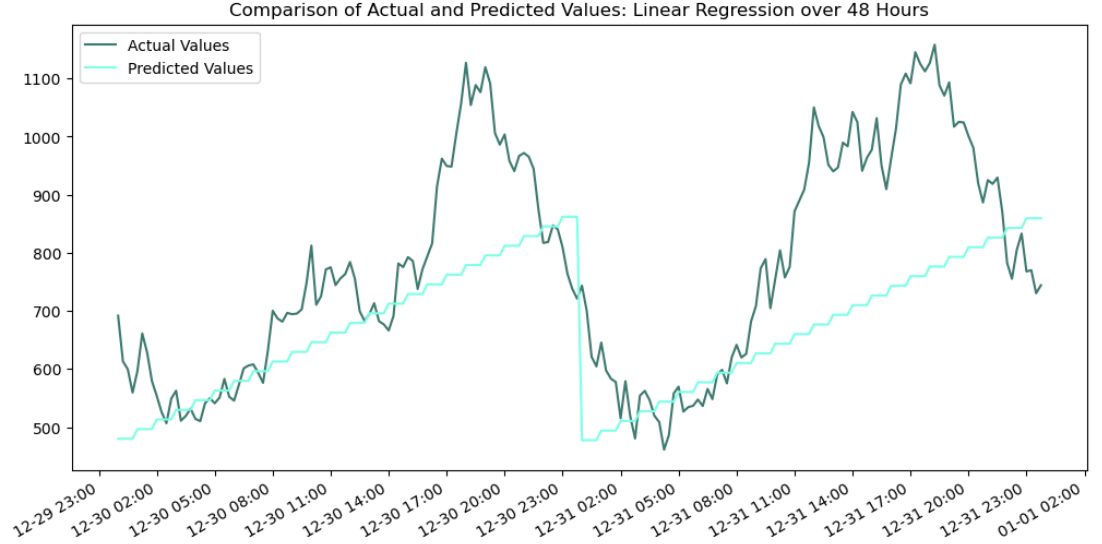
\includegraphics[width=13.75cm,keepaspectratio]{./images/Lineare_Regression_ueber_48_Stunden_mit_.png}
\caption{Lineare Regression über 48 Stunden mit Energieverbrauchsdaten und Meteodaten als Input}
\small~\textit{(Quelle: Eigene Darstellung).}
\label{fig:lineare_regression_ueber_48_stunden_mit_energieverbrauchsdaten_und_meteodaten_als_input}
\end{figure}
Das zweite Modell nutzt lediglich die Energieverbrauchsdaten von 2021 bis 2023 mit dem Lastgang und die daraus abgeleiteten Variablen 'Lastgang\_Moving\_Average' und 'Lastgang\_First\_Difference'. Es verwendet keine zusätzlichen Features aus externen Datensätzen. Die Modellzusammenfassung weist ein R\^\{2\}-Wert von 0.382 auf. Das heisst, dass ungefähr 38.2 \% der Varianz der tatsächlichen Lastgangwerte durch das Modell erklärt werden. Da der p-Wert bei 0.00 liegt, zeigt das Modell trotz moderater Modellanpassung eine signifikante Erklärungskraft. Das bedeutet, dass das Modell über zufällige Schätzungen hinaus eine Beziehung zwischen Zeitvariablen und Lastgang aufzeigt. Die Berechnung des MAPE ist mit 19.61 \% leicht höher im Vergleich zur ersten Konfiguration mit zusätzlichen Meteodaten.

Der Code zu diesem Modell ist auf \href{https://huggingface.co/Sari95/Linear-Regression-for-Energy-Consumption-Prediction}{Hugging Face} unter dem Namen Linear-Regression-for-Energy-Consumption-Prediction abrufbar.


\subsubsection{SARIMAX}\label{subsubsec:sarimax}
SARIMAX ist eine erweiterte Methode der autoregressiven integrierten gleitenden Durchschnitte (ARIMA), welche als Input externe Variablen zulässt.

Zuerst wurden die Hyperparameter basierend auf der Analyse des Autokorrelationsfunktionen (ACF)-Plots, des partiellen Autokorrelationsfunktionen (PACF)-Plots sowie des Stationaritätstests wie dem Augmented-Dickey-Fuller (ADF)-Tests bestimmt. Nach den Vorverarbeitungsschritten, die in \vref{subsec:anwendung_der_machine_learning_modelle} vorgestellt sind, wurden die Daten auf Werte zwischen 0 und 1 skaliert. Anschliessend wurden die externen Variablen aus dem Meteodatensatz sowie die beiden aus den Energieverbrauchsdaten erzeugten Features 'Lastgang\_Moving\_Average' und 'Lastgang\_First\_Difference' zum Modell hinzugefügt. Das angewendete Modell nutzt als Input die Energieverbrauchsdaten und die Meteodaten lediglich von 2023, da eine grössere Menge an Inputdaten zum Absturz der Berechnungen geführt hat. Nachdem die Inputdaten definiert waren, wurde das Modell trainiert und schlussendlich genutzt, um Vorhersagen zu generieren. Diese Vorhersagen wurden danach auf ihre ursprüngliche Grösse zurückskaliert.

Die ACF- und PACF-Plots in Abbildung \ref{fig:autokorrelationsfunktion_und_partielle_autokorrelationsfunktion_des_lastgangs_fuer_das_definieren_de} visualisieren das Abklingen der Autokorrelationen mit der Zeit. Der ACF-Plot zeigt zu Beginn einen starken Abfall, der anschliessend langsamer abklingt. Dieses Muster bedeutet, dass es eine starke positive Autokorrelation mit früheren Werten gibt, die mit der Zeit abnimmt. Ausserdem weist dieses Muster darauf hin, dass eine AR-Komponente benötigt wird. Im PACF-Plot ist ein hoher erster Lag und anschliessend ein starker Abfall ersichtlich. Dieses Muster weist auf einen AR(1)-Prozess hin, da nur die erste Verzögerung signifikant ist. Anschliessend gehen die partiellen Korrelationen schnell gegen null. 


\begin{figure}[h!]
\centering
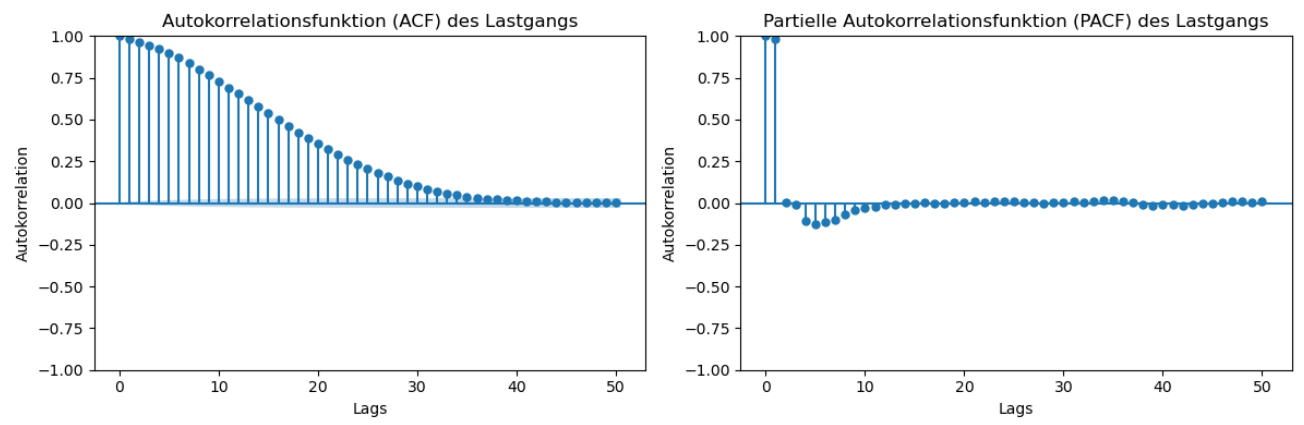
\includegraphics[width=13.75cm,keepaspectratio]{./images/Autokorrelationsfunktion_und_partielle_A.png}
\caption{Autokorrelationsfunktion und partielle Autokorrelationsfunktion des Lastgangs für das Definieren der SARIMAX-Hyperparameter}
\small~\textit{(Quelle: Eigene Darstellung).}
\label{fig:autokorrelationsfunktion_und_partielle_autokorrelationsfunktion_des_lastgangs_fuer_das_definieren_de}
\end{figure}
Anhand dieser Ergebnisse und den im \vref{subsubsec:energieverbrauchsdaten_im_15_minuten_intervall_2021_bis_2023} präsentierten Analysen wurden die folgenden Hyperparameter für das SARIMAX-Modell festgelegt:

\begin{itemize}
    \item Die Parameter (p, d, q) wurden auf (1,0,0) gesetzt: Die autoregressive Komponente p wurde aufgrund des schnellen Abfalls der partiellen Autokorrelation nach dem ersten Lag auf 1 gesetzt. Die Differenzierung d wurde auf 0 gesetzt, da die Zeitreihe der Energieverbrauchsdaten gemäss des ADF-Tests stationär ist. Es wurde keine Moving Average Komponente q genutzt, da die Autokorrelationsfunktion nach dem initialen Abfall langsam absinkt und keine signifikanten Spitzen aufweist.

    \item Die Parameter (P, D, Q, s) wurden auf (1,0,0,96) gesetzt: Die autoregressive Komponente P wurde auf 1 gesetzt, damit das Modell saisonale Autokorrelation erkennt und den saisonalen Lag vom Zyklus s zur Vorhersage verwendet. Die saisonale Differenzierung D wurde ebenfalls auf 0 gesetzt, da basierend auf dem Resultat des ADF-Tests von Stationarität in der Zeitreihe ausgegangen wird. Die saisonale Moving Average Komponente Q wurde nicht verwendet. Die Saisonalität s wurde auf 96 gesetzt, um die tägliche Saisonalität der 15-Minuten-Intervalle zu berücksichtigen.

\end{itemize}

Die Fehlermetriken zeigen für das SARIMAX-Modell ein MSE von 14060.03 \(kW^{2}\), ein MAE von 82.81 kW, ein RMSE von 118.57 kW und einen MAPE von 9.91 \%. Der AIC liegt für dieses Modell bei -148'917.25. Der BIC liegt bei -148'815.77.


In der Visualisierung  \ref{fig:sarimax_ueber_48_stunden_mit_energieverbrauchsdaten_und_meteodaten_als_input} der tatsächlichen und prognostizierten Werte über die 48 Stunden hinweg ist zu sehen, dass das Modell das Muster der Daten grundsätzlich erfasst. Abweichungen sind jedoch von blossem Auge erkennbar - insbesondere am zweiten Tag zwischen 11.00 Uhr und 18.00 Uhr.


\begin{figure}[h!]
\centering
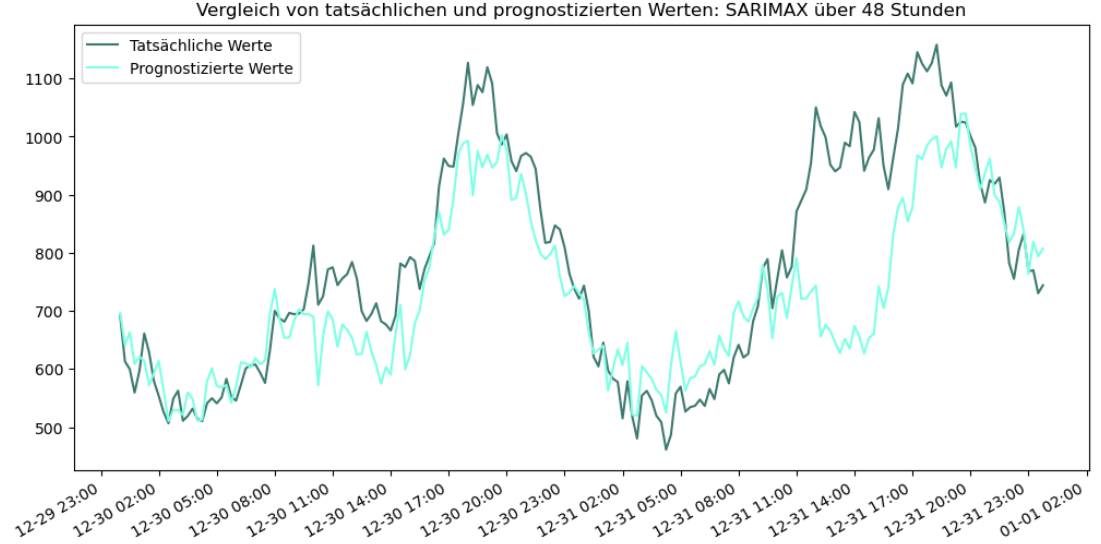
\includegraphics[width=13.75cm,keepaspectratio]{./images/SARIMAX_ueber_48_Stunden_mit_Energieverb.png}
\caption{SARIMAX über 48 Stunden mit Energieverbrauchsdaten und Meteodaten als Input}
\small~\textit{(Quelle: Eigene Darstellung).}
\label{fig:sarimax_ueber_48_stunden_mit_energieverbrauchsdaten_und_meteodaten_als_input}
\end{figure}
Der Code zu diesem Modell ist auf \href{https://huggingface.co/Sari95/SARIMAX-for-Energy-Consumption-Prediction}{Hugging Face}  unter dem Namen SARIMAX-for-Energy-Consumption-Prediction abrufbar.


\subsubsection{Exponential Smoothing}\label{subsubsec:exponential_smoothing}
Exponential Smoothing zeichnet sich durch eine Glättung der Zeitreihendaten unter Berücksichtigung einer exponentiell abnehmenden Gewichtung vergangener Beobachtungen aus. Aktuelleren Werten wird dabei eine höhere Beachtung als länger vergangenen Werten geschenkt \cite{DatacampSARIMAForecasting}. Das angewendete Triple Exponential Smoothing nutzt lediglich die Energieverbrauchsdaten von 2021 bis 2023 mit dem Lastgang als Input, da dem Modell keine weiteren Features mitgegeben werden können. Das Modell verwendet eine additive saisonale Komponente mit einer Saisonlänge von 96. Dieser Wert entspricht einem Tag, da die Energieverbrauchsdaten in 15-Minuten-Intervallen vorliegen.


Die Fehlermetriken weisen ein MSE von 17633.18 \(kW^{2}\), ein MAE von 93.12 kW und ein RMSE von 132.79 kW auf. Der MAPE von 10.74 \% zeigt, dass die Prognosen durchschnittlich eine Abweichung von etwas mehr als 10 \% haben. Die Werte für AIC und BIC dieses Modells betragen 794'397.83 beziehungsweise 795'334.81.


In der Visualisierung  \ref{fig:triple_exponential_smoothing_ueber_48_stunden_mit_energieverbrauchsdaten_als_input} der tatsächlichen und prognostizierten Werte ist ersichtlich, dass das Modell die generellen Muster und Trends der tatsächlichen Daten erfasst. Visuelle Abweichungen sind jedoch deutlich erkennbar. Die Werte in den frühen Morgenstunden wie auch die Werte in den Abendstunden werden zu tief vorhergesagt. Insbesondere in den zweiten 24 Stunden ist die Differenz in den Stunden zwischen 11.00 Uhr und 18.00 Uhr sehr deutlich erkennbar.


\begin{figure}[h!]
\centering
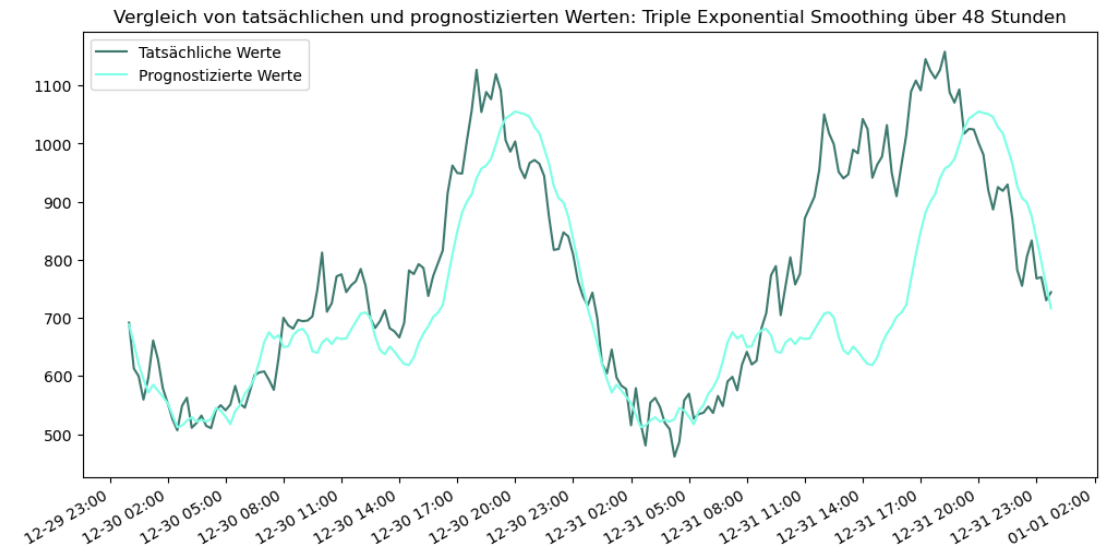
\includegraphics[width=13.75cm,keepaspectratio]{./images/Triple_Exponential_Smoothing_ueber_48_St.png}
\caption{Triple Exponential Smoothing über 48 Stunden mit Energieverbrauchsdaten als Input}
\small~\textit{(Quelle: Eigene Darstellung).}
\label{fig:triple_exponential_smoothing_ueber_48_stunden_mit_energieverbrauchsdaten_als_input}
\end{figure}
Der Code zu diesem Modell ist auf \href{https://huggingface.co/Sari95/Exponential-Smoothing-for-Energy-Consumption-Prediction}{Hugging Face} unter dem Namen Exponential-Smoothing-for-Energy-Consumption-Prediction abrufbar.


\subsubsection{TBATS}\label{subsubsec:tbats}
TBATS steht für Trigonometrische Saisonalität, Box-Cox-Transformation, ARMA-Fehler, Trend und saisonale Komponente. Die Methode scheint gemäss Literatur besonders geeignet zu sein für Zeitreihen mit mehrfachen saisonalen Mustern, wie in \vref{subsec:verwandte_arbeiten} zu lesen ist. Das vorliegende Modell nutzt eine Kombination aus Box-Cox-Transformation, ARMA-Fehlern und trigonometrischer Saisonalität, um die Komplexität der saisonalen Muster in den Energieverbrauchsdaten zu erfassen. Die saisonalen Perioden wurden auf tägliche und wöchentliche Muster eingestellt, was 96 beziehungsweise 672 15-Minuten-Intervalle entsprechen. Die Box-Cox-Transformation wurde mit 'use\_box\_cox=False' deaktiviert, da der ADF-Test aus \vref{subsec:explorative_datenanalyse__eda_} die Stationarität der Zeitreihe bestätigte. Zudem wurde die ARMA-Fehlerkomponente mit 'use\_arma \_errors=False' deaktiviert, da die Einbeziehung zu einem etwas höherem MAPE (10.12~\%) geführt hat.


Die Evaluationsmetriken zeigen für das TBATS-Modell ein MSE von 16455.89 \(kW^{2}\), ein MAE von 85.23 kW, ein RMSE von 128.28 kW und einen MAPE-Wert von rund 10 \% (9.996~\%). Ein MAPE von etwa 10 \% zeigt, dass die Vorhersagen des TBATS-Modells im Durchschnitt recht präzise sind. Die Werte für AIC und BIC dieses Modells betragen 2'004'401.12 beziehungsweise 791'370.13.


Die Visualisierung \ref{fig:tbats_ueber_48_stunden_mit_energieverbrauchsdaten_als_input} bestätigt diese Ergebnisse. Das TBATS-Modell fängt die allgemeinen Muster und Schwankungen der tatsächlichen Daten mehrheitlich gut ein. Sichtbare Abweichungen entstehen hauptsächlich zu den Spitzenzeiten, insbesondere in den zweiten 24 Stunden zwischen 11.00 Uhr und 18.00 Uhr.


\begin{figure}[h!]
\centering
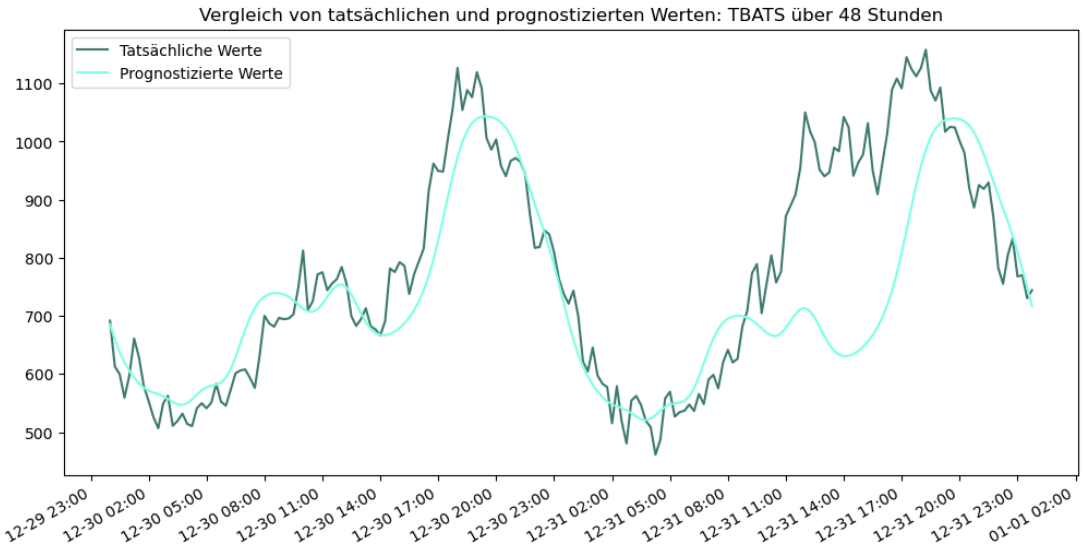
\includegraphics[width=13.75cm,keepaspectratio]{./images/TBATS_ueber_48_Stunden_mit_Energieverbra.png}
\caption{TBATS über 48 Stunden mit Energieverbrauchsdaten als Input}
\small~\textit{(Quelle: Eigene Darstellung).}
\label{fig:tbats_ueber_48_stunden_mit_energieverbrauchsdaten_als_input}
\end{figure}
Der Code zu diesem Modell ist auf \href{https://huggingface.co/Sari95/TBATS-for-Energy-Consumption-Prediction}{Hugging Face} unter dem Namen TBATS-for-Energy-Consumption-Prediction abrufbar.

\subsubsection{LSTM}\label{subsubsec:lstm}
Wie dem \vref{subsec:machine_learning_modelle_zur_prognose_von_zeitreihendaten} zu entnehmen ist, sind LSTM-Modelle in der Lage, langfristige Abhängigkeiten zu lernen und scheinen sich daher besonders gut für komplexe Vorhersageaufgaben wie die Lastgangprognose zu eignen. Die LSTM-Architektur wurde mit der PyTorch-Bibliothek implementiert, welche die Möglichkeit bietet, Operationen mit Tensoren durchzuführen und das Training unter Verwendung von GPUs zu beschleunigen. Nach den Vorverarbeitungsschritten, die in \vref{subsec:anwendung_der_machine_learning_modelle} vorgestellt sind, wurden die Daten auf Werte zwischen 0 und 1 skaliert. Nach der Aufteilung in Trainings- und Testdaten wurden mehrere Epochen durchlaufen, um die Hyperparameter des Netzes anzupassen und das Modell auf die Vorhersage der Lastgangwerte abzustimmen. Am Ende wurden die Werte wieder in ihre ursprüngliche Grösse zurückskaliert.

Das angewendete LSTM-Modell wurde als Klasse 'LSTMModel' konzipiert. Die Klasse erbt von 'nn.Module', der Basisklasse für alle neuronalen Netzwerke in PyTorch \cite{ChatGPTCodeLSTM}. Im Konstruktor '\_\_init\_\_' wurden drei wesentliche Parameter definiert: 'input\_size', die Dimension der Eingabedaten, 'hidden\_layer\_size', die Grösse der versteckten Schicht, und 'output\_size', die Dimension der Ausgabedaten des Modells. Das Modell umfasst eine LSTM-Schicht 'self.lstm', die für die Verarbeitung der Eingabesequenz sowie des initialen Zustands der versteckten Schichten zuständig ist. Diese Schicht gibt sequenziell Ausgabewerte sowie einen aktualisierten versteckten Zustand zurück. Zusätzlich wurde eine lineare Schicht 'self.linear' integriert, welche die Ausgabe der LSTM-Schicht anpasst, um die gewünschte Ausgabegrösse zu erreichen \cite{UnderstandingLSTMArchitecture}. Die 'forward'-Methode definiert den Verarbeitungsprozess der Eingaben, wobei die Ausgabe der LSTM-Schicht an die lineare Schicht weitergeleitet wird  \cite{ChatGPTCodeLSTM}. Die lineare Schicht erzeugt schliesslich die finale Vorhersage für jede Sequenz. Eine Instanz des Modells wurde mit den Parametergrössen 7, 100 und 1 erstellt und für den Einsatz auf eine GPU geladen. Die Modellarchitektur nutzt die Fähigkeiten der LSTM-Zellen zur Verarbeitung von Sequenzen mit zeitlichen Abhängigkeiten, indem sie relevante Informationen über verschiedene Zeitintervalle speichert oder vergisst. Die Eingabeschicht nimmt skalierte Features auf, die an die versteckten LSTM-Schichten weitergeleitet werden, welche die Daten verarbeiten und an die Ausgabeschicht weitergeben, um die finale Prognose zu liefern.


Die Fehlermetriken zeigen für das LSTM-Modell sehr gute Ergebnisse: Der MSE beträgt 1517.03 \(kW^{2}\), der MAE 30.37 kW und der RMSE 38.95 kW. Für den MAPE ergibt sich ein Wert von 3.93 \%. Aus diesen Metriken lässt sich eine hohe Vorhersagegenauigkeit der Energieverbrauchswerte über 48 Stunden durch das LSTM-Modell schliessen. Diese Genauigkeit hebt die LSTM-Methode von den bisherigen Methoden deutlich ab.


Die visuelle Darstellung der tatsächlichen und prognostizierten Werte in Abbildung \ref{fig:lstm_ueber_48_stunden_mit_energieverbrauchsdaten_und_meteodaten_als_input} verdeutlicht die Metriken. Das LSTM-Modell ist in der Lage, die Muster der Lastgangwerte präzise zu erfassen und nahe an den tatsächlichen Verläufen zu prognostizieren. Eine deutliche Verbesserung der Vorhersagegenauigkeit gegenüber den vorherigen Modellen Exponential Smoothing und TBATS zeigt sich insbesondere in den zweiten 24 Stunden zwischen 11.00 Uhr und 18.00 Uhr, in denen die statistischen Modelle Schwierigkeiten hatten, das Muster zu erfassen.


\begin{figure}[h!]
\centering
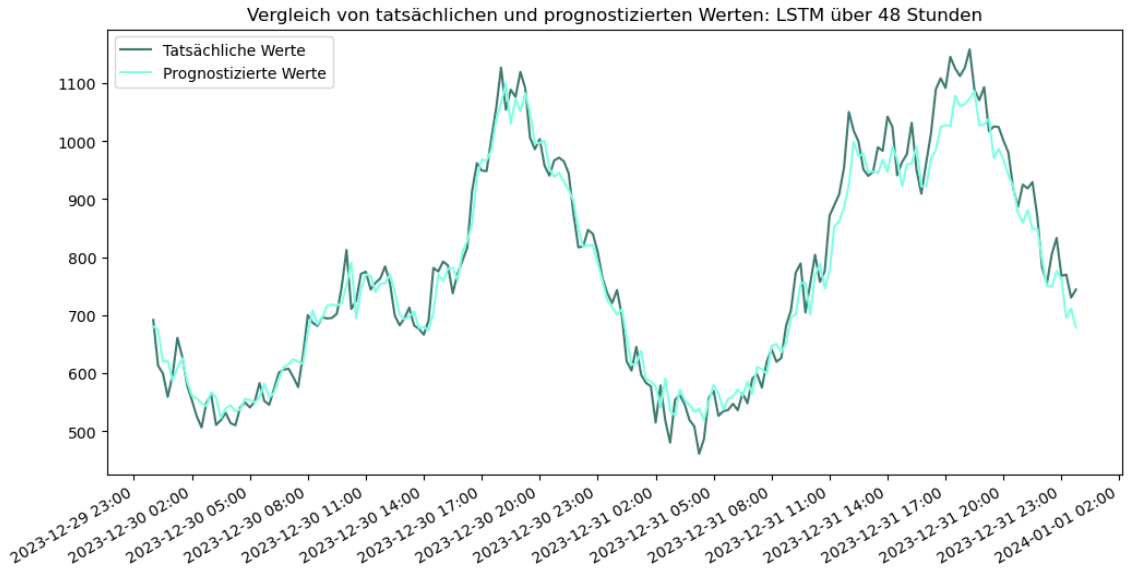
\includegraphics[width=13.75cm,keepaspectratio]{./images/LSTM_ueber_48_Stunden_mit_Energieverbrau.png}
\caption{LSTM über 48 Stunden mit Energieverbrauchsdaten und Meteodaten als Input}
\small~\textit{(Quelle: Eigene Darstellung).}
\label{fig:lstm_ueber_48_stunden_mit_energieverbrauchsdaten_und_meteodaten_als_input}
\end{figure}
In einer zweiten Modellkonfiguration wurde die gleiche LSTM-Architektur verwendet, jedoch mit einer Reduktion des 'input\_size' von sieben auf drei Variablen. Dadurch wurden als Inputdaten nur die Energieverbrauchsdaten und die daraus abgeleiteten Variablen 'Lastgang\_Moving\_Average' und 'Lastgang\_First\_Difference', ohne Meteodaten genutzt. Alle anderen Einstellungen wurden übernommen. Der MAPE-Wert zeigte sich bei dieser Konfiguration mit 4.02 \% nur geringfügig höher im Vergleich zur vorherigen Konfiguration mit zusätzlichen Meteodaten.

Der Code zu diesem Modell ist auf \href{https://huggingface.co/Sari95/LSTM-for-Energy-Consumption-Prediction}{Hugging Face}  unter dem Namen LSTM-for-Energy-Consumption-Prediction abrufbar.

\subsubsection{Transformer}\label{subsubsec:transformer}
Transformer-Architekturen haben sich in der jüngsten Forschung für die Verarbeitung von Zeitreihendaten als äusserst effektiv erwiesen, wie in \vref{subsec:verwandte_arbeiten} nachzulesen ist. Bei der Transformer-Architektur sind insbesondere die Mechanismen der Self-Attention und des Positional Encodings hervorzuheben. Dadurch kann das Modell die Bedeutung der Daten in einer Sequenz erfassen und die Reihenfolge der Zeitreihendaten erfassen. Im Gegensatz zu LSTM-Modellen, die sequenzielle Daten Datenpunkt für Datenpunkt verarbeiten, können Transformer die gesamte Datenreihe auf einmal betrachten und Beziehungen zwischen weit auseinanderliegenden Punkten effektiv modellieren \cite{ArticleTransformerforTimeSeriesModels}.


Im angewendeten Modell wurden als Input die Energieverbrauchs- und die Meteodaten von 2021 bis 2023 sowie die beiden zusätzlichen Features 'Lastgang\_Moving\_Average' und 'Lastgang\_First\_Difference' verwendet. Nach den Vorverarbeitungsschritten, die in \vref{subsec:anwendung_der_machine_learning_modelle} vorgestellt sind, wurden die Daten mit dem MinMaxScaler aus der Bibliothek scikit-learn auf Werte zwischen 0 und 1 skaliert. Weiter wurde den Trainingsdaten mit einer definierten Funktion Positional Encoding hinzugefügt. Transformer-Modelle können von Natur aus keine Informationen über die Reihenfolge der Daten in einer Sequenz verarbeiten, da sie alle Eingaben gleichzeitig verarbeiten \cite{ArticleTransformerforTimeSeriesModels}. Dieser Schritt war daher notwendig, damit das Modell die zeitliche Dimension der Daten erkennen kann und ein Verständnis der Reihenfolge innerhalb der Sequenz bekommen kann. Nach der Aufteilung in ein Trainings- und Testset wurde das Transformer-Modell auf einem 'cuda'-fähigen Gerät trainiert. Dadurch konnte die beschleunigte Verarbeitung durch die GPU verwendet werden. Das Training des Modells erfolgte in Epochen, wobei der frühe Abbruch, auch Early Stopping genannt, zur Vermeidung von Overfitting eingesetzt wurde. Das Modell ist mit einem Transformer-Encoder, einer Einbettungsschicht und einer finalen linearen Schicht aufgebaut. Am Ende wurden die Werte wieder in ihre ursprüngliche Grösse zurückskaliert.


Im verwendeten Modell wurde zunächst eine Klasse 'TransformerModel' definiert, die von 'nn.Module' erbt. Dies stellt die Basisklasse für alle neuronalen Netzwerke in PyTorch dar \cite{ChatGPTCodeTransformer}. Im Konstruktor '\_\_init\_\_' wurden grundlegende Parameter festgelegt: 'input\_size' für die Grösse der Eingabe, 'hidden\_layer\_size' für die Grösse der versteckten Schichten, 'output\_size' für die Ausgabegrösse, 'num\_layers' für die Anzahl der Transformer-Layer und 'nhead' für die Anzahl der Attention-Köpfe. Eine Embedding-Schicht wurde genutzt, um die Eingabefeatures in eine höhere Dimension umzuwandeln, die durch 'hidden\_layer\_size' definiert ist. Die Anwendung des Transformer-Encoders, der die Attention-Mechanismen verwendet, ermöglichte es, alle Informationen aus der Sequenz gleichzeitig zu erfassen und so komplexe Muster in den Daten zu erkennen. Nach der Verarbeitung durch den Encoder reduzierte eine lineare Schicht die Dimensionalität auf die gewünschte Ausgabegrösse \cite{UnderstandingTransformerArchitecture}. Die 'forward'-Methode wurde definiert, um den Datenfluss durch das Modell zu regeln \cite{ChatGPTCodeTransformer}. Abschliessend wurde eine Instanz des Modells mit den Parametern 7, 100, 1 und 2 erstellt und für den Einsatz auf einer GPU vorbereitet.


Die Fehlermetriken liegen für den MSE bei 1531.46 \(kW^{2}\), für den MAE bei 29.30 kW und für den RMSE bei 39.13 kW. Das Modell zeigt einen MAPE von 3.93 \%. Diese Werte bestätigen die Präzision des Transformer-Modells im Vergleich zu den vorher vorgestellten Modellen.


Die Visualisierung \ref{fig:transformer_ueber_48_stunden_mit_energieverbrauchsdaten_und_meteodaten_als_input} zeigt, dass das Transformer-Modell den allgemeinen Trend und die täglichen Muster der Lastgangwerte erfolgreich nachbildet. Die Vorhersagen erzielen über den Zeitraum von 48 Stunden eine hohe Übereinstimmung mit den tatsächlichen Werten. 


\begin{figure}[h!]
\centering
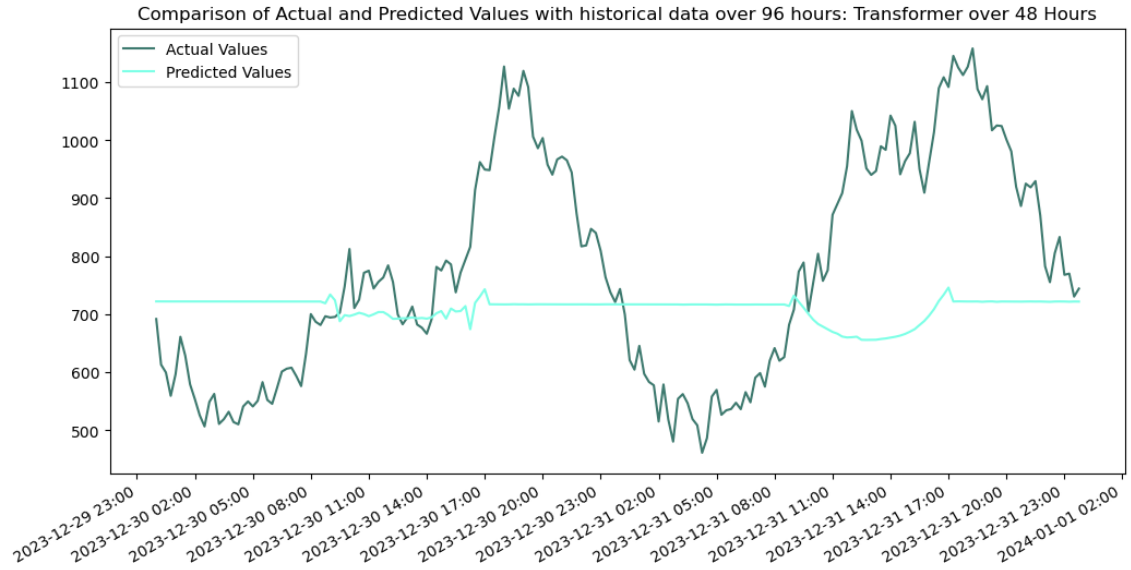
\includegraphics[width=13.75cm,keepaspectratio]{./images/Transformer_ueber_48_Stunden_mit_Energie.png}
\caption{Transformer über 48 Stunden mit Energieverbrauchsdaten und Meteodaten als Input}
\small~\textit{(Quelle: Eigene Darstellung).}
\label{fig:transformer_ueber_48_stunden_mit_energieverbrauchsdaten_und_meteodaten_als_input}
\end{figure}
In einem weiteren Schritt der Analyse wurde die Eingabedimension des Transformer-Modells von sieben auf drei Variablen verringert. Dadurch wurden als Input nur die Energieverbrauchsdaten und die daraus abgeleiteten Variablen 'Lastgang\_Moving\_Average' und 'Lastgang\_First\_Difference' genutzt, ohne Meteodaten. Die restlichen Modellparameter wurden unverändert gelassen. Die modifizierte Konfiguration resultierte in einem etwas höheren MAPE von 5.2 \% als die vorherige Konfiguration mit zusätzlichen Meteodaten.

Der Code zu diesem Modell ist auf \href{https://huggingface.co/Sari95/Transformer-Architecture-for-Energy-Consumption-Prediction}{Hugging Face} unter dem Namen Transformer-Architecture-for-Energy-Consumption-Prediction abrufbar.


\subsection{Evaluation und Vergleich der Machine Learning-Modelle}\label{subsec:evaluation_und_vergleich_der_machine_learning_modelle}
Im letzten Schritt erfolgte die Evaluation anhand von 5 definierten Kriterien, die in diesem Kapitel detailliert vorgestellt werden. Die Evaluation zielte darauf ab, die effektivsten Modelle für präzise Energieverbrauchsprognosen zu identifizieren und die Leistungsfähigkeit der verschiedenen Ansätze zu vergleichen. Ein zentrales Kriterium war die Vorhersagegenauigkeit des Lastgangs in 15-Minuten-Intervallen, gemessen am MAPE-Wert über 48 Stunden. Dies beinhaltet insbesondere die Fähigkeit eines Modells, den Energieverbrauch mit möglichst geringer Abweichung von den realen Werten vorherzusagen. Weitere Bewertungskriterien schlossen die Modellkomplexität und Anpassungsgüte ein. Zudem wurde untersucht, ob bestimmte Zeiten innerhalb der 48 Stunden durch eine stärkere Abweichung auffielen. Hinsichtlich des Rechen- und Zeitaufwands wurde die Effizienz des Modells bezüglich der benötigten Ressourcen berücksichtigt. Dabei wurde der Arbeitsspeicherverbrauch in Megabyte und die CPU- beziehungsweise GPU-Auslastung gemessen. Und schliesslich wurde die Ausführungszeit erfasst. Zusätzlich wurde evaluiert, ob die Modelle die Möglichkeit haben, externe Features wie Meteoinformationen zu integrieren. Abschliessend erhielten die Modelle eine Bewertung zwischen 0 und 10, welche die Gesamteignung des Modells beschreibt, um Energieverbrauchsdaten als Zeitreihendaten über kurze Zeitstpannen zu prognostizieren. Die Bewertung 10 bedeutet, dass sich das Modell eignet, um Zeitreihendaten in 15-Minuten-Intervallen über 48 Stunden vorherzusagen. Die Tabelle \ref{tab:EvalutationMLModelle} zeigt die Bewertung der angewendeten Modelle anhand dieser fünf Kriterien:


\begin{landscape}~


\begin{center}
\footnotesize
\begin{longtable}{|p{3.2cm}|p{2.9cm}|p{3.1cm}|p{2.9cm}|p{3.1cm}|p{2.5cm}|p{2.5cm}|}
\hline
 & \textbf{Lineare Regression} & \textbf{SARIMAX} & \textbf{Exponential Smoothing} & \textbf{TBATS} & \textbf{LSTM} & \textbf{Transformer} \\
\hline
\textbf{Anpassungsgüte - Fehlermetriken}

 & MSE: 29459.06

MAE: 144.13

RMSE: 171.64

MAPE: 19.29 \%

 & MSE: 14060.03

MAE: 82.81

RMSE: 118.57

MAPE: 9.91 \%

 & MSE: 17633.18

MAE: 93.12

RMSE: 132.79

MAPE: 10.74 \%

 & MSE: 16455.89

MAE: 85.23

RMSE: 128.28

MAPE: 9.996 \%

 & MSE: 1517.03

MAE: 30.37

RMSE: 38.95

MAPE: 3.93 \%

 & MSE: 1531.46

MAE: 29.30

RMSE: 39.13

MAPE: 3.93 \%

 \\
\hline
\textbf{Modellkomplexität} & AIC: -1.656e+05

BIC: -1.656e+05

\(R^{2}\)-Wert: 0.46

 & AIC: -148'917.25

BIC: -148'815.77

 & AIC: 794'397.83

BIC: 795'334.81

 & AIC: 2'004'401.12

BIC: 791'370.13

 & Anzahl Schichten: 1

Anzahl versteckte Schichten: 100

 & Anzahl Schichten: 2

Anzahl versteckte Schichten: 100

 \\
\hline
\textbf{Graphische Analyse der Vorhersagegenauigkeit} & Die Spitzen und Senken des Energieverbrauchs können nicht erfasst werden. & Abweichungen sind von blossem Auge erkennbar - insbesondere am zweiten Tag zwischen 11.00 Uhr und 18.00 Uhr. & In den zweiten 24 Stunden ist die Differenz in den Stunden zwischen 11.00 Uhr und 18.00 Uhr sehr deutlich erkennbar. & In den zweiten 24 Stunden ist die Differenz in den Stunden zwischen 11.00 Uhr und 18.00 Uhr sehr deutlich erkennbar. & Kaum sichtbare Abweichungen. Die Spitze in den zweiten 24 Stunden zwischen 16.00 und 19.00 Uhr zeigt eine Differenz. & Kaum sichtbare Abweichungen. \\
\hline
\textbf{Ressourcen}

\textbf{aufwand}

\textbf{1)}~\textbf{ Arbeitsspeicherverbrauch}

\textbf{2)}~\textbf{Auslastung CPU / GPU}

\textbf{3)}~\textbf{Ausführungszeit}

 & \begin{enumerate}
    \item 338.77 MB

    \item 26.2 \% über 16 CPUs

    \item 36 Sekunden

\end{enumerate}

 & \begin{enumerate}
    \item 106.51 GB

    \item 74.1 \% über 16 CPUs

    \item 7133 Sekunden = ca. 2 Stunden 

\end{enumerate}

 & \begin{enumerate}
    \item  283.33 MB

    \item  95 \% über 16 CPUs

    \item 31 Sekunden

\end{enumerate}

 & \begin{enumerate}
    \item  2.46 GB

    \item 98.2 \% über 16 CPUs

    \item 2401 Sekunden = ca. 40 Minuten

\end{enumerate}

 & \begin{enumerate}
    \item  24.31 GB

    \item GPU 1: 23 \%, GPU 2: 100 \%

    \item 234 Sekunden = ca. 4 Minuten

\end{enumerate}

 & \begin{enumerate}
    \item  34.7 GB

    \item GPU 1: 24 \%, GPU 2: 55 \%

    \item 460 Sekunden = ca. 7.5 Minuten

\end{enumerate}

 \\
\hline
\textbf{Zusätzliche Vorverarbeitungsschritte der Daten} & Skalierung der Daten & Skalierung der Daten, Überprüfung ACF- und PACF-Plot & Keine & Keine & Skalierung der Daten, Umwandlung in PyTorch-Tensoren & Skalierung der Daten, Umwandlung in PyTorch-Tensoren \\
\hline
\textbf{Integration externer Faktoren } & Möglich & Möglich

 & Nicht möglich & Nicht möglich & Möglich & Möglich \\
\hline
\textbf{Insgesamte Bewertung (1-10)} & 1 & 3 & 6 & 5 & 10 & 10 \\
\hline
\caption{Bewertung der 6 angewendeten Machine und Deep Learning-Modelle}
\label{tab:EvalutationMLModelle}\\
\end{longtable}
\end{center}\begin{center}
\footnotesize
\textit Training Ratio: Alle Tage bis auf die letzten 48 h (Zeitraum Januar 2021 - Dezember 2023)\\ Verwendete Ressourcen: AMD EPYC 7313P 16-Core Prozessor, 146 GB Arbeitsspeicher, 2 NVIDIA A100 80GB PCIe Grafikkarten (betrieben mit CUDA-Version 12.4)\\ Inputdaten sind die Energieverbrauchsdaten und Meteodaten von 2021 - 2023 - Ausnahme SARIMAX mit Inputdaten von 2023

\end{center}

\end{landscape}~


\section{Diskussion und Fazit}\label{sec:diskussion_und_fazit}
Dieses Kapitel umfasst die abschliessende Diskussion sowie das Fazit der Arbeit. Zunächst werden die vorgestellten Ergebnisse interpretiert, im Kontext der vorgestellten Literatur eingebettet und Limitierungen der Ergebnisse beschrieben. Anschliessend wird aufgezeigt, was die vorliegende Studie beantworten konnte und es folgt ein Ausblick für zukünftige Forschungsbereiche.

\subsection{Zusammenfassung und Bewertung der Forschungsergebnisse}\label{subsec:zusammenfassung_und_bewertung_der_forschungsergebnisse}
Die exploratorische Datenanalyse in \vref{subsec:explorative_datenanalyse__eda_} zeigt einen durchschnittlichen Energieverbrauch von 676.31 kW mit einer Standardabweichung von 219.77 kW, was auf eine moderate bis hohe Variabilität hindeutet. Die Daten weisen eine Normalverteilung mit Schiefe zu höheren Werten auf. Es lässt sich schliessen, dass die Energiebranche neben dem durchschnittlichen auch gelegentlichen hohen Energiebedarf decken können muss. Die Visualisierungen zur Zeitreihenanalyse sowie zur Autokorrelation zeigen typische saisonale Schwankungen im Energieverbrauch - mit niedrigerem Verbrauch im Sommer und in der Nacht sowie höherem im Winter und in den Abendstunden. Die Korrelationsanalyse zwischen Meteodaten und dem Lastgang zeigt überwiegend schwache bis mässige negative Korrelationen. Insbesondere bei Variablen, welche die Sonnenstrahlung messen. Diese negativen Korrelationen deuten auf geringeren Energiebedarf an sonnenreichen Tagen mit gleichzeitiger höherer Energieproduktion durch Photovoltaikanlagen hin.

Die lineare Regression hat mit einem MAPE von 19.29 \% sowie mit sichtbaren Abweichungen in der Visualisierung verdeutlicht, dass sie die tägliche Saisonalität in den Energieverbrauchsdaten nicht adäquat erfassen kann und nicht geeignet ist, um eine vernünftige Vorhersage von Lastgangwerten über den Zeitraum von 48 Stunden aufzustellen. Trotzdem zeichnet sich dieses Modell durch seine Effizienz aus, indem es Vorhersagen innerhalb von weniger als einer Minute geliefert hat. Weiter ist die einfache Konzeption schnell zu verstehen. Beim Vergleich verschiedener, fortgeschrittener Machine Learning- und Deep Learning-Methoden dient die lineare Regression häufig als Basisgrundlage \cite{OreillyDataScienceBuch}. Das Modell bietet somit einen wertvollen Referenzpunkt zur Bewertung der Leistungssteigerung durch die komplexeren Algorithmen. Zudem ist die lineare Regression ein geeigneter Ausgangspunkt, um die Variablen für die Modellintegration zu definieren.


Beim SARIMAX-Modell war der hohe Ressourcenaufwand nicht zu rechtfertigen, um 15-Minuten-Intervalle über 48 Stunden aus 3 Jahren historischer Daten vorherzusagen. Auch der Einsatz der auto-arima-Funktion 'pm.auto\_arima()' zur Bestimmung der optimalen Modellparameter erwies sich aufgrund des erheblichen Ressourcenbedarfs als nicht effizient. In der Literatur wird SARIMAX häufig für seine Fähigkeit gelobt, komplexe zeitliche Dynamiken zu modellieren \cite{BookTimeSeriesAnalysis}. Die erzielten Resultate im Rahmen dieser Arbeit liessen jedoch eine tiefere und detailliertere Beschäftigung mit dem SARIMAX-Modell als nicht sinnvoll erscheinen. Insbesondere auch aufgrund der Tatsache, dass andere in dieser Arbeit vorgestellte Modelle mit weniger Ressourcenaufwand bessere Ergebnisse lieferten. 


Die Anwendung des Triple Exponential Smoothing-Modells hat einen MAPE von 10.74 \%  ergeben und zeigt somit eine deutliche Verbesserung gegenüber der linearen Regression. Zudem spricht auch die notwendige Zeit von 31 Sekunden für das Modell, um die Vorhersagen zu generieren. Das TBATS-Modell zeichnet mit einem MAPE von 9.996 \% wie auch visuell eine sehr ähnliche Situation wie das Triple Exponential Smoothing-Modell. Beide Modelle stellen einen bedeutenden Fortschritt gegenüber dem einfacheren Modell der linearen Regression sowie dem SARIMAX-Modell dar. TBATS weist mit einem AIC von 2'004'401.12 auf ein komplexeres Modell hin als das Exponential Smoothing-Modell (794'397.83). Im Hinblick auf den zeitlichen Aufwand zeigt TBATS mit ungefähr 40 Minuten einen deutlich höheren Ressourcenaufwand. Sichtbare Abweichungen entstehen bei beiden Modellen hauptsächlich zu den Spitzenzeiten, insbesondere in den zweiten 24 Stunden zwischen 11.00 Uhr und 18.00 Uhr. Abschliessend ist zu sagen, dass die beiden Modelle eine robuste Vorhersagefähigkeit zeigen. Jedoch werden für präzisere Prognosen, insbesondere für den zweiten Tag, komplexere Modelle benötigt. Aufgrund der geringeren Komplexität sowie der deutlich kürzeren Zeitdauer ist zu schlussfolgern, dass sich das Triple Exponential Smoothing-Modell besser eignet, um eine vernünftige Vorhersage von Lastgangwerten über den Zeitraum von 48 Stunden aufzustellen.

Das LSTM- wie auch das Transformer-Modell trumpfen mit ihren MAPE-Werten von 3.93~\% mit einer sehr präzisen Vorhersagegenauigkeit. Insbesondere die Genauigkeit in den zweiten 24 Stunden fällt im Vergleich zu den beiden vorherigen statistischen Modellen auf. Mit einem Zeitaufwand von ungefähr 4 Minuten beim LSTM-Modell sowie von ungefähr 7.5 Minuten beim Transformer-Modell ist die Zeitdauer für die Berechnungen bei den vorhandenen Ressourcen als sehr vernünftig einzuschätzen. Ein Blick auf die bestehende Literatur in \vref{subsec:verwandte_arbeiten} zeigt, dass neuere Forschungsergebnisse eine hohe Genauigkeit von LSTM- und Transformer-Modellen in der Vorhersage komplexer Zeitreihen dokumentieren. Die erzielten Ergebnisse bestätigen die Leistungsfähigkeit in diesem Anwendungsbereich. Die Modelle übertreffen die herkömmlichen statistischen Verfahren und liefern präzise Prognosen mit einem angemessenen Rechenaufwand. Überrascht hat das Resultat, dass die Vorhersagegenauigkeit bei den beiden Modellen ohne die Variablen aus den Meteodaten nur minimal beeinträchtigt wurde. Abschliessend kann die Anwendung des LSTM-Modells sowie der Transformer-Architektur im Rahmen dieser Studie als Erfolg betrachtet werden, um eine vernünftige Vorhersage von Lastgangwerten über den Zeitraum von 48 Stunden aufzustellen.


Die Ergebnisse zeigen, dass sowohl die LSTM- als auch die Transformer-Modelle eine höhere Vorhersagegenauigkeit erreichen als die traditionellen statistischen Methoden, die in der vorliegenden Studie betrachtet wurden. Diese Ergebnisse bestätigen die Erkenntnisse aus der Literatur, die in \vref{subsec:verwandte_arbeiten} ausgeführt sind. Die Literatur bewertet den Einsatz von Deep Learning-Techniken für die Prognose von Zeitreihendaten im Energieverbrauch als geeignete Methoden \cite{ArticleReviewDLTechniques}. Ein interessanter Aspekt ist der vergleichsweise geringe Einfluss der Meteodaten auf die Vorhersagegenauigkeit, wie die geringfügige Verbesserung der MAPE-Werte impliziert. Dies könnte darauf hindeuten, dass Meteodaten auf die Vorhersage von Daten aus Transformatorenstationen weniger Einfluss haben oder dass die beiden Deep Learning-Modelle bereits ausreichend robust sind, um ohne diese zusätzlichen Informationen genaue Vorhersagen zu treffen. Limitierungen der Ergebnisse ergeben sich daraus, dass auf die Verwendung eines Validierungssets verzichtet wurde, was die Generalisierbarkeit der Ergebnisse leicht beeinträchtigt. Des Weiteren wurden die Modelle für die Vorhersage der 15-Minuten-Intevalle über einen Zeitraum von 48 Stunden getestet, was keine Rückschlüsse auf die Vorhersagegenauigkeit für andere kurzfristige Zeiträume wie 2 bis 14 Tage zulässt. 


\subsection{Diskussion des Forschungsbeitrags und Ausblick auf zukünftige Forschungen}\label{subsec:diskussion_des_forschungsbeitrags_und_ausblick_auf_zukuenftige_forschungen}
Dieses Kapitel erörtert den Beitrag der Studie zu den aufgezeigten Forschungslücken und skizziert mögliche Ansätze für zukünftige Forschungen. Diese Arbeit zeigt trotz vielversprechender Ergebnisse der verwendeten Modelle mehrere Bereiche auf, die weitere Untersuchungen benötigen.

Die Arbeit hat sich zum Ziel gesetzt, die nachfolgende Forschungsfrage zu beantworten und hat in \vref{subsubsec:forschungsluecke_und_forschungsfrage} sieben grosse Forschungslücken identifiziert:

\begin{mdframed}[backgroundcolor=gray!20, innertopmargin=10pt, innerbottommargin=10pt, innerleftmargin=10pt, innerrightmargin=10pt, rightmargin=15pt, skipabove=10pt, skipbelow=10pt, linewidth=0pt]
\textit{FF: Welche Machine Learning-Modelle eignen sich am besten für die Prognose von Zeitreihendaten des Energieverbrauchs aus Schweizer Transformatorenstationen?}

\end{mdframed}

Im Mittelpunkt der Forschungsfrage stand die Vorhersagegenauigkeit anhand des MAPE-Wertes über zwei Tage. Zusammenfassend lässt sich festhalten, dass die Weiterentwicklung von LSTM- und Transformer-Modellen besonders vielversprechend erscheint, da sie die präzisesten Prognosen geliefert haben. Dennoch sollten statistische Modelle nicht vollständig ausser Acht gelassen werden, insbesondere in Umgebungen, wo keine leistungsfähigen GPUs verfügbar sind, um komplexe Berechnungen effizient durchzuführen.

Zur Forschungslücke 1 konnte zudem einen Beitrag geleistet werden, indem die Studie robuste Prognosen durch zwei Deep Learning-Modelle generiert hat. Diese Modelle demonstrieren, wie die Integration von Echtzeitdaten aus Smart Metern optimiert werden kann, um bestehende Datenlücken zu schliessen, die durch die aktuelle Gesetzgebung und Trägheit verschiedener IT-Systeme entstehen. Ein weiterer Beitrag konnte zur Forschungslücke 2 beigetragen werden, indem die Leistung und Effizienz von fünf State-of-the-Art-Modellen umfassend verglichen wurde. Die Ergebnisse haben gezeigt, dass insbesondere die Deep Learning-Modelle mit MAPE-Werten unter 5 \% sehr präzise Vorhersagen ermöglichen, während statistische Modelle wie das Exponential Smoothing durch geringen Ressourcenverbrauch bei gleichzeitiger guter Vorhersagegenauigkeit überzeugen. Des Weiteren wurde ein Beitrag zur Forschungslücke 5 durch die Integration von Meteodaten in die Modelle erbracht. Jedoch konnte nicht abschliessend geklärt werden, wie stark dieser Einfluss tatsächlich ist und ob er signifikant ist. In Bezug auf Forschungslücke~6 wurde ein weiterer Beitrag geleistet, indem nicht nur die Vorhersagegenauigkeit, sondern auch der Ressourcenaufwand und die Modellkomplexität evaluiert wurden. Es hat sich gezeigt, dass die verwendeten LSTM- und Transformer-Architekturen einen geringen Aufwand erfordern, sofern leistungsfähige Grafikkarten zur Verfügung stehen. Zudem erzielen Exponential Smoothing- mit geringem und TBATS-Modelle mit akzeptablem Ressourcenaufwand gute Ergebnisse. 


Zukünftige Forschungsrichtungen sollten die folgenden noch offenen Fragen adressieren:

\begin{enumerate}
    \item Die Frage, inwieweit Meteodaten die kurzfristige Vorhersagegenauigkeit des Energieverbrauchs beeinflussen, benötigt weitere Untersuchungen. Insbesondere gilt es zu klären, ob Meteodaten einen signifikanten Einfluss auf die Genauigkeit dieser Prognosen haben und wie gross dieser Einfluss ist. Die Ergebnisse aus den \mbox{Deep} Learning-Modellen, die ohne Einbeziehung der Meteodaten durchgeführt wurden, zeigten nur eine geringe Verschlechterung des MAPE-Wertes. Dies legt nahe, dass der Einfluss von Meteodaten möglicherweise geringer ist, als ursprünglich angenommen. Ein kürzlich aufgetretenes Ereignis in der Schweizer Energieversorgung widerspricht jedoch diesem Ergebnis und unterstreicht die potenzielle Bedeutung von Wetterprognosen. Nach unerwartetem Schneefall, der auf warme Apriltage folgte, waren Photovoltaikanlagen schneebedeckt. Dies führte zu einem drastischen Einbruch der Solarstromproduktion - entgegen den Stromprognosen. Als Folge musste die Netzgesellschaft Swissgrid den Strommangel durch teure Zukaufe kompensieren \cite{NZZFehlprognosenSolarstrom}. Dieses Beispiel zeigt, dass Wetterprognosen einen entscheidenden Einfluss auf Prognosewerte haben können und hebt die Bedeutung der weiteren Forschung in diesem Bereich hervor. 
    \item Eine detailliertere Überprüfung ist notwendig, um die Forschungslücke 4 zu adressieren. Dabei sollte untersucht werden, ob die Einbeziehung von Energieproduktionsdaten durch Haushalte zu anderen Ergebnissen führt, insbesondere im Hinblick auf den zukünftig weiter fortschreitenden Ausbau von Photovoltaikanlagen.

    \item Der Miteinbezug weiterer zeitbezogener Variablen könnte insbesondere bei statistischen Modellen die Vorhersagegenauigkeit verbessern. In der vorliegenden Studie wurden die beiden zusätzlichen Variablen 'Lastgang\_Moving\_Average’ und ’Lastgang\_First\_Difference’ aus dem Energieverbrauchsdatensatz berücksichtigt. Weitere zeitbezogene Variablen wie Tageszeit, Wochentag, Ferien- und Feiertage wurden nicht einbezogen. Ein vorläufiger Test mit der linearen Regression, bei dem zwei zusätzliche zeitbezogene Variablen berücksichtigt wurden, führte zu einer messbaren Verbesserung des MAPE-Wertes. Da eine ausführliche Präsentation dieser Ergebnisse den Umfang dieser Arbeit überschreiten würde, können die Resultate aus den ersten Tests in \vref{sec:ergebnisse_der_linearen_regression_mit_zeitbezogenen_variablen} eingesehen werden.

    \item Die Kombination von LSTM mit anderen Modellen wie CNNs, die in der Literatur in \vref{subsec:verwandte_arbeiten} zu erfolgsversprechenden Ergebnissen geführt hat, sollte weiter erforscht werden. In der vorliegenden Arbeit wurde von einem kombinierten Ansatz abgesehen, da die LSTM-Architektur bereits sehr vernünftige Resultate geliefert hat.

    \item Die Leistungsfähigkeit der Modelle bei längeren Vorhersagezeiträumen als 48 Stunden sollte überprüft werden, um die Forschungslücke 3 zu adressieren. 
    \item Um Forschungslücke 7 zu adressieren, sollte untersucht werden, wie die Modelle effektiv in reale Anwendungen integriert werden können. Trotz der hohen Rechenanforderungen von Deep Learning-Modellen waren Laufzeit und Ressourcenverbrauch in dieser Studie praktikabel, was ihren Einsatz in realen Anwendungen ermöglicht. Hierbei sollte die Frage geklärt werden, wie viele historische Daten es braucht, ohne dass die Vorhersagegenauigkeit stark beeinträchtigt wird. Vorläufige erste Tests haben gezeigt, dass mindestens 3 Monate an Daten erforderlich sind, um einen MAPE von unter 10 \% zu erreichen. Da eine ausführliche Darstellung dieser Resultate den Umfang dieser Arbeit überschreiten würde, sind die Ergebnisse dieser ersten Tests in \vref{sec:ergebnisse_der_transformer_architektur_mit_unterschiedlicher_laenge_an_historischen_daten} zu finden.

\end{enumerate}

Abschliessend liefert diese Arbeit wertvolle Erkenntnisse für die wissenschaftliche Gemeinschaft durch den Vergleich und die Bewertung verschiedener Machine Learning- und Deep Learning-Modelle im spezifischen Kontext der Schweizer Energiebranche. Der praktische Nutzen dieser Arbeit ermöglicht es Energieversorgungsunternehmen, anhand der Verwendung dieser Modelle die beschriebene Datenlücke aufgrund gesetzlicher Grundlagen oder der Trägheit von IT-Systemen zu schliessen. Die gewonnenen Erkenntnisse können zudem genutzt werden, um Prognosen über den Energieverbrauch mittels Machine Learning-Modellen zu verbessern. Dies ist im Hinblick auf den Ausbau der erneuerbaren Energien von entscheidender Wichtigkeit, wie das jüngste Beispiel von schneebedeckten Photovoltaikanlagen illustriert hat.

\newpage  

\section*{Deklaration}\label{sec:deklaration}
\addcontentsline{toc}{section}{Deklaration}
\textbf{Die Länge des vorliegenden Textes ab und inklusive Kapitelüberschrift 1 bis vor diesen Abschnitt beträgt 14'334 Wörter.}

Ich bestätige, die vorliegende Arbeit selbständig verfasst zu haben. Sämtliche Textstellen, die nicht von mir stammen, sind als Zitate gekennzeichnet und mit dem genauen Hinweis auf ihre Herkunft versehen. Die verwendeten Quellen (gilt auch für Abbildungen, Grafiken u.ä.) sind im Literatur- bzw. Quellenverzeichnis aufgeführt.

Ich bestätige weiterhin, dass ich bei der Erstellung dieser Studienarbeit durchgehend steuernd gearbeitet habe und von einer KI erzeugte Texte bzw. Textfragmente nicht unreflektiert übernommen habe.

22. Mai 2024,

\begin{figure}[H]

\includegraphics[width=3.5cm,height=2cm,keepaspectratio]{./images/Unterschrift.png}
\label{fig:unterschrift}
\end{figure}
Sarah Schürch

\newpage  
\renewcommand{\refname}{Quellen}
\addcontentsline{toc}{section}{Quellen}
\setcounter{biburllcpenalty}{7000}
\setcounter{biburlucpenalty}{8000}
\printbibliography
\appendix  
\newpage  
\section*{Glossar}\label{sec:glossar}
\addcontentsline{toc}{section}{Glossar}
In diesem Kapitel sind Fachwörter und ihre Erklärung zu finden, die zum Verständnis der vorliegenden Arbeit beitragen. Die Begriffe sind alphabetisch aufgelistet.

\textbf{Convolutional Neural Network (CNN)}\\
CNN ist ein tiefes neuronales Netzwerk, das insbesondere in der Bildverarbeitung und -erkennung eingesetzt wird, indem es Muster in Bildern erkennt \cite{TowardsDataScienceCNN}. 


\textbf{Energieverbrauch in Kilowattstunde (kWh) und in Kilowatt (kW)}\\
Der Energieverbrauch misst die genutzte Energiemenge, die über einen bestimmten Zeitraum hinweg verbraucht wird \cite{BMWKEnergiewende}. Eine Kilowattstunde entspricht der Energie, die ein Kilowatt-Gerät eine Stunde benötigt. Es ist eine standardisierte Einheit, um beispielsweise den Energieverbrauch von Haushalten und Unternehmen zu messen \cite{Paschotta2010}. Kilowatt (kW) hingegen ist eine Einheit für die Leistung \cite{EKZKWvsKWH}.


\textbf{Exponential Smoothing}\\
Exponential Smoothing ist ein Zeitreihenvorhersagemodell, welches aktuellere Beobachtungen stärker gewichtet als ältere. Dadurch sollen zukünftige Werte genauer prognostiziert werden \cite{sktimeDocuExponentialSmoothing}. Weitere Ausführungen sind in \vref{subsubsec:exponential_smoothing} zu finden. 


\textbf{Long Short-Term Memory (LSTM)}\\
LSTM bezeichnet ein rekurrentes neuronales Netzwerk, das speziell dafür entwickelt wurde, langfristige Abhängigkeiten in Daten zu erkennen und zu lernen \cite{geeksforgeeksLSTM}. Ausführlichere Informationen sind in \vref{subsubsec:lstm} zu finden. 


\textbf{Machine Learning}\\
Bezeichnet einen Unterbereich der künstlichen Intelligenz, der Algorithmen verwendet, um aus Daten zu lernen und Vorhersagen oder Entscheidungen ohne explizite Programmierung zu treffen \cite{BigDataInsiderML}. 


\textbf{Overfitting und Underfitting}\\
Overfitting bedeutet, dass ein Modell die Trainingsdaten zu gut lernt. Dadurch kann das Modell schlecht auf neue, unbekannte Daten generalisieren. Underfitting hingegen tritt auf, wenn ein Modell weder die Trainingsdaten noch unbekannte Daten adäquat modellieren kann. Dies tritt meistens auf, weil das Modell zu einfach ist \cite{OverfittingUnderfittingGeeksforGeeks}.


\textbf{PyTorch}\\
Die Open Source-Bibliothek wurde vom Facebook AI Research Lab entwickelt. Sie ist besonders für ihre Flexibilität und Benutzerfreundlichkeit in der Anwendung von Machine Learning bekannt. Die Bibliothek integriert sich nahtlos in die Programmiersprache Python \cite{PythonFrameworks}.


\newpage~


\textbf{Positional Encoding}\\
Positional Encoding wird insbesondere in Transformer-Modellen verwendet, um Informationen über die Position von Elementen innerhalb einer Sequenz hinzuzufügen. Es ermöglicht dem Modell, die Reihenfolge der Datenpunkte zu berücksichtigen, da Transformer-Modelle von Natur aus eine Unterscheidung der Sequenzabfolge treffen \cite{ArticlePositionalEncoding}.


\textbf{Regressionsanalyse}\\
Die Regressionsanalyse ist eine statistische Methode zur Modellierung der Beziehung zwischen einer abhängigen Variable und einer oder mehreren unabhängigen Variablen \cite{UZHLineareRegression}. Dadurch kann die Stärke des Zusammenhangs quantifiziert werden und Vorhersagen über die abhängige Variable getroffen werden \cite{ScribbrLineareRegression}. Ausführlichere Informationen sind in \vref{subsubsec:lineare_regression} zu finden. 


\textbf{Seasonal ARIMA (SARIMA)}\\
SARIMA erweitert ARIMA um die Komponente der Saisonalität. Es stellt ein Zeitreihenmodell dar, welches aus den Komponenten Saisonalität (S), Autoregression (AR), Integration (I) und gleitende Durchschnitte (MA) kombiniert, um Daten mit saisonalen Mustern zu modellieren \cite{DatacampSARIMAForecasting}. Weitere Informationen sind in \vref{subsubsec:sarimax} zu finden.


\textbf{Smart Meter}\\
Smart Meter messen und übermitteln Verbrauchsdaten für Versorgungsleistungen wie Strom. Im Vergleich zu traditionellen Zählern können sie 15-Minuten-Lastgänge senden und detailliertere Verbrauchsinformationen bereitstellen \cite{EnergieCHSmartMeter}. Weitere Ausführungen sind in \vref{subsec:energiesystem} zu finden.


\textbf{Supervised Learning}\\
Supervised Learning bezeichnet ein Machine Learning-Ansatz, bei dem Modelle anhand von bereits gelabelten Trainingsdaten trainiert werden. Das Modell lernt die Beziehung zwischen Eingabedaten und ihren zugeordneten Ausgaben (z.B. Klassifizierung und Regression) \cite{IBMSupervisedUnsupervisedLearning}. 


\textbf{TBATS}\\
TBATS ist ein Zeitreihenmodell, um komplexe saisonale Muster zu handhaben. Der Begriff setzt sich aus den Komponenten Trigonometric seasonality (T), Box-Cox transformation (B), ARMA errors (A), Trend (T) und Seasonal components (S) zusammen \cite{sktimeDocuTBATS}. Ausführlichere Informationen sind in \vref{subsubsec:tbats} zu finden. 


\textbf{Trafostationen / Transformatorenstation / Netzstation}\\
Eine Trafostation transformiert elektrische Energie von einem Mittelspannungsnetz in ein Niederspannungsnetz zur allgemeinen Versorgung \cite{SwissgridNetzebenenTrafostation}. Weitere Informationen sind in \vref{subsec:energiesystem} zu finden.


\newpage~


\textbf{Transformer-Methoden}\\
Transformer Methoden sind eine Klasse von Modellen, bei denen Aufmerksamkeitsmechanismen verwendet werden, um Beziehungen zwischen allen Worten in einem Satz zu erfassen. Diese Methode wird häufig in der Verarbeitung natürlicher Sprache verwendet \cite{TowardsDataScienceTransformers}. Ausführlichere Informationen sind in \vref{subsubsec:transformer} zu finden. 


\textbf{Unsupervised Learning}\\
Unsupervised Learning bezeichnet ein Machine Learning-Ansatz, bei dem Modelle anhand ungelabelten Daten trainiert werden, um Muster oder Strukturen in den Daten selbständig zu erkennen. Beispielsweise fallen Clusteringsaufgaben darunter \cite{IBMSupervisedUnsupervisedLearning}. 


\textbf{Zeitreihendaten / Time Series-Data}\\
Zeitreihendaten bestehen aus sequenziellen Messungen, die über Zeitintervalle hinweg erfasst werden. Jeder Messpunkt ist einem eindeutigen Zeitpunkt zugeordnet. Daten in dieser Art ermöglichen die Analyse von Veränderungen und Trends über die Zeit und werden in verschiedenen Bereichen angewendet, um Muster zu erkennen und Vorhersagen zu treffen \cite{OreillyZeitreihendatenBuch}. Zeitreihendatenbanken sind auf die Verwaltung sequenzieller Datenpunkte spezialisiert, die über die Zeit gesammelt werden\cite{DunningFriedman2014}. Typische Vertreter dieses Datenbanktyps sind InfluxDB, TimescaleDB oder Prometheus. Weitere Ausführungen sind in \vref{subsec:zeitreihendaten} zu finden. 


\appendix~

\newpage~

\renewcommand{\thesection}{\Alph{section})}

\section*{Anhang}\label{sec:anhang}
\addcontentsline{toc}{section}{Anhang}
\section{Quellcode der Machine Learning- und Deep Learning-Modelle}\label{sec:quellcode_der_machine_learning__und_deep_learning_modelle}
Im Folgenden sind Code-Ausschnitte der verwendeten Modelle gezeigt. Sie zeigen die Aufteilung in Trainings- und Testdaten sowie die Erstellung des jeweiligen Modells. Zur besseren Übersichtlichkeit ist der vollständige Quellcode auf HuggingFace hinterlegt, wobei die entsprechenden Links Quellcode angegeben sind.

\textbf{Lineare Regression}\\
Der folgende Code zeigt ein grundlegendes Beispiel, wie eine lineare Regression mit Python durchgeführt werden kann. Der gesamte Code zu diesen Modellkonfigurationen ist auf \href{https://huggingface.co/Sari95/Linear-Regression-for-Energy-Consumption-Prediction}{Hugging Face}  unter dem Namen \textit{Linear-Regression-for-Energy-Consumption-Prediction} abrufbar.


\begin{mdframed}[backgroundcolor=gray!20, innertopmargin=10pt, innerbottommargin=10pt, innerleftmargin=10pt, innerrightmargin=10pt, rightmargin=15pt, skipabove=10pt, skipbelow=10pt, linewidth=0pt]
\footnotesize
\textit{\#\#Durchführung einer linearen Regression mit Energieverbrauchsdaten und Meteodaten Jahr 2021-2023}\\
\textit{\# Aufteilung der Daten in Trainings- und Testdaten}\\
\textit{\# Die letzten 192 Datenpunkte (48 Stunden bei 15-Minuten-Intervallen) sind der Testdatensatz}\\
\textit{train = dfEnergyAll.iloc[:-192]}\\
\textit{test = dfEnergyAll.iloc[-192:]}

\textit{\# Definieren der Ziel- und erklärenden Variablen für Training und Test}\\
\textit{y\_train = train['Lastgang']}\\
\textit{X\_train = train[['StundenwertStrahlung', 'Globalstrahlung\_15Min', 'StrahlungGeneigteFläche', }

\textit{'TheorPVProd', 'Direktnormalstrahlung', 'Schönwetterstrahlung', 'Lufttemperatur', }\\ \textit{'Lastgang\_Moving\_Average', 'Lastgang\_First\_Difference']]}\\
\textit{X\_train = sm.add\_constant(X\_train)}


\textit{y\_test = test['Lastgang']}\\
\textit{X\_test = test[['StundenwertStrahlung', 'Globalstrahlung\_15Min', 'StrahlungGeneigteFläche', 'TheorPVProd', 'Direktnormalstrahlung', 'Schönwetterstrahlung', 'Lufttemperatur', }\\ \textit{'Lastgang\_Moving\_Average', 'Lastgang\_First\_Difference']]}\\
\textit{X\_test = sm.add\_constant(X\_test)}


\textit{\# Erstellen und Anpassen des Modells mit Trainingsdaten}\\
\textit{model = sm.OLS(y\_train, X\_train).fit()}

\textit{\# Vorhersagen für Testdaten erstellen}\\
\textit{predictions = model.predict(X\_test)}

\end{mdframed}  

\vspace{0.5cm}

\newpage~


\textbf{SARIMAX}\\
Der nachfolgende Code zeigt eine beispielhafte Erstellung eines SARIMAX-Modells mit Python. Der gesamte Code zu diesem Modell ist auf \href{https://huggingface.co/Sari95/SARIMAX-for-Energy-Consumption-Prediction}{Hugging Face} unter dem Namen \textit{SARIMAX-for-Energy-Consumption-Prediction} zu finden.


\begin{mdframed}[backgroundcolor=gray!20, innertopmargin=10pt, innerbottommargin=10pt, innerleftmargin=10pt, innerrightmargin=10pt, rightmargin=15pt, skipabove=10pt, skipbelow=10pt, linewidth=0pt]
\footnotesize
\textit{\#\#Durchführung SARIMAX mit Energieverbrauchsdaten und Meteodaten Jahr 2021-2023}\\
\textit{\# Index als DatetimeIndex setzen und die passende Frequenz definieren (hier 15-Minuten-Intervalle)}\\
\textit{dfEnergyAll = dfEnergyAll.asfreq('15T')}

\textit{\# Aufteilung der Daten in Trainings- und Testdaten}\\
\textit{\# Die letzten 192 Datenpunkte (48 Stunden bei 15-Minuten-Intervallen) sind der Testdatensatz}\\
\textit{train, test = train\_test\_split(dfEnergyAll, train\_size=len(dfEnergyAll)-192)}

\textit{\# Definieren der Ziel- und erklärenden Variablen für Training und Test}\\
\textit{y\_train = train['Lastgang']}\\
\textit{X\_train = train[['StundenwertStrahlung', 'Lufttemperatur', 'Globalstrahlung\_15Min', 'StrahlungGeneigteFläche', 'Lastgang\_Moving\_Average', 'Lastgang\_First\_Difference']]}

\textit{y\_test = test['Lastgang']  \# Wird später für die Evaluation verwendet}\\
\textit{X\_test = test[['StundenwertStrahlung', 'Lufttemperatur', 'Globalstrahlung\_15Min', 'StrahlungGeneigteFläche', 'Lastgang\_Moving\_Average', 'Lastgang\_First\_Difference']]  \# Wird für die Vorhersage verwendet}

\textit{\# Erstellen \& Anpassen des SARIMAX-Modells und Training}\\
\textit{\# SARIMAX-Modell mit ARIMA(1,0,0) und saisonaler Ordnung (1,0,0,96)}\\
\textit{model = sm.tsa.SARIMAX(y\_train, exog=X\_train, order=(1,0,0), seasonal\_order=(1,0,0,96),}\\
\textit{enforce\_stationarity=False, enforce\_invertibility=False)}\\
\textit{results = model.fit()}

\textit{\# Modell für Vorhersagen nutzen (192 Steps für 48 Stunden-Vorhersagen)}\\
\textit{predictions = results.get\_forecast(steps=192, exog=X\_test).predicted\_mean}

\end{mdframed}  

\vspace{0.5cm}
\textbf{Exponential Smoothing}\\
Der folgende Code zeigt beispielhaft die Anwendung des Triple Exponential Smoothing-Modells mit Python. Der gesamte Code zu diesem Modell ist auf \href{https://huggingface.co/Sari95/Exponential-Smoothing-for-Energy-Consumption-Prediction}{Hugging Face} unter dem Namen \textit{Exponential-Smoothing-for-Energy-Consumption-Prediction} abrufbar.


\begin{mdframed}[backgroundcolor=gray!20, innertopmargin=10pt, innerbottommargin=10pt, innerleftmargin=10pt, innerrightmargin=10pt, rightmargin=15pt, skipabove=10pt, skipbelow=10pt, linewidth=0pt]
\footnotesize
\textit{\#\#Durchführung Triple Exponential Smoothing mit Energieverbrauchsdaten Jahr 2021-2023}\\
\textit{\# Trainingsgrösse (Alle Daten bis auf die letzten 48 Stunden) und Testgrösse (48 Stunden) definieren}\\
\textit{train\_size = len(dfEnergyAll) - (2 * 24 * 4)  }\\
\textit{test\_size = 2 * 24 * 4  }

\textit{\# Aufteilung in Trainings- und Testdaten}\\
\textit{train\_data = dfEnergyAll['Lastgang'][:train\_size]}\\
\textit{test\_data = dfEnergyAll['Lastgang'][train\_size:]}

\textit{\# Modellinitialisierung und Training}\\
\textit{\# Berücksichtigung additiver saisonaler Komponente und 96 als Periode für tägliche Saisonalität (bei 15-Minuten-Intervalle)}\\
\textit{model = ExponentialSmoothing(train\_data, seasonal='add', seasonal\_periods=96)}\\
\textit{fitted\_model = model.fit()}

\textit{\# Vorhersagen erstellen in der Länge der Testgrösse (48 Stunden)}\\
\textit{y\_forecast = fitted\_model.forecast(steps=test\_size)}

\textit{\# Vorhersageergebnisse mit Zeitstempeln versehen}\\
\textit{forecast\_series = pd.Series(y\_forecast, index=test\_data.index)}

\end{mdframed}  

\vspace{0.5cm}
\textbf{TBATS}\\
Die folgende Code zeigt beispielhaft, wie ein TBATS-Modell mit Python angewendet wird. Der gesamte Code zu diesem Modell ist auf \href{https://huggingface.co/Sari95/TBATS-for-Energy-Consumption-Prediction}{Hugging Face} unter dem Namen \textit{TBATS-for-Energy-Consumption-Prediction} zu finden.


\begin{mdframed}[backgroundcolor=gray!20, innertopmargin=10pt, innerbottommargin=10pt, innerleftmargin=10pt, innerrightmargin=10pt, rightmargin=15pt, skipabove=10pt, skipbelow=10pt, linewidth=0pt]
\footnotesize
\textit{\#\#Durchführung TBATS mit Energieverbrauchsdaten Jahr 2021-2023}\\
\textit{\# Trainingsgrösse (Alle Daten bis auf die letzten 48 Stunden) und Testgrösse (48 Stunden) definieren}\\
\textit{train\_size = len(dfEnergyAll) - (2 * 24 * 4)  }\\
\textit{test\_size = 2 * 24 * 4  }

\textit{\# Aufteilung in Trainings- und Testdaten}\\
\textit{train\_data = dfEnergyAll['Lastgang'][:train\_size]}\\
\textit{test\_data = dfEnergyAll['Lastgang'][train\_size:]}

\textit{\# Modellinitialisierung und Training}\\
\textit{\# 96 als Periode für tägliche Saisonalität, 672 als Periode für wöchentliche Saisonalität (bei 15-Minuten-Intervalle}\\
\textit{estimator = TBATS(seasonal\_periods=[96, 672], use\_arma\_errors=False, use\_box\_cox=False)}\\
\textit{fitted\_model = estimator.fit(train\_data)}

\textit{\# Vorhersagen erstellen in der Länge der Testgrösse (48 Stunden)}\\
\textit{y\_forecast = fitted\_model.forecast(steps=test\_size)}

\textit{\# Vorhersageergebnisse mit Zeitstempeln versehen}\\
\textit{last\_timestamp = dfEnergyAll.index[train\_size - 1]}\\
\textit{future\_timestamps = pd.date\_range(start=last\_timestamp, periods=test\_size + 1, freq='15T')[1:]}\\
\textit{forecast\_series = pd.Series(y\_forecast, index=future\_timestamps)}

\end{mdframed}  

\vspace{0.5cm}
\textbf{LSTM}\\
Der folgende Code zeigt beispielhaft einen Teil aus der LSTM-Architektur mit Python und PyTorch. Der gesamte Code zu diesen Modellkonfigurationen ist auf \href{https://huggingface.co/Sari95/LSTM-for-Energy-Consumption-Prediction}{Hugging Face} unter dem Namen \textit{LSTM-for-Energy-Consumption-Prediction} abrufbar.


\begin{mdframed}[backgroundcolor=gray!20, innertopmargin=10pt, innerbottommargin=10pt, innerleftmargin=10pt, innerrightmargin=10pt, rightmargin=15pt, skipabove=10pt, skipbelow=10pt, linewidth=0pt]
\footnotesize
\textit{\# LSTM-Modell erstellen}\\
\textit{class LSTMModel(nn.Module):}\\
\textit{     def \_\_init\_\_(self, input\_size, hidden\_layer\_size, output\_size):}\\
\textit{        super(LSTMModel, self).\_\_init\_\_()}\\
\textit{        self.hidden\_layer\_size = hidden\_layer\_size}\\
\textit{        self.lstm = nn.LSTM(input\_size, hidden\_layer\_size, batch\_first=True)}\\
\textit{        self.linear = nn.Linear(hidden\_layer\_size, output\_size)}

\textit{    def forward(self, input\_seq, hidden\_state):}\\
\textit{        lstm\_out, hidden\_state = self.lstm(input\_seq, hidden\_state)}\\
\textit{        predictions = self.linear(lstm\_out[:, -1, :])}\\
\textit{        return predictions, hidden\_state}

\# Modell instanziieren \\
\textit{model = LSTMModel(7, 100, 1).to(device)  }

\end{mdframed}  

\vspace{0.5cm}
\textbf{Transformer}\\
Der folgende Block zeigt beispielhaft einen Code-Ausschnitt aus der Transformer-Architektur mit Python und PyTorch. Der gesamte Code zu diesen Modellkonfigurationen ist auf \href{https://huggingface.co/Sari95/Transformer-Architecture-for-Energy-Consumption-Prediction}{Hugging Face} unter dem Namen \textit{Transformer-Architecture-for-Energy-Consumption-Prediction} abrufbar.


\begin{mdframed}[backgroundcolor=gray!20, innertopmargin=10pt, innerbottommargin=10pt, innerleftmargin=10pt, innerrightmargin=10pt, rightmargin=15pt, skipabove=10pt, skipbelow=10pt, linewidth=0pt]
\footnotesize
\textit{\# Transformer-Modell erstellen}\\
\textit{class TransformerModel(nn.Module):}\\
\textit{     def \_\_init\_\_(self, input\_size, hidden\_layer\_size, output\_size, num\_layers, nhead):}\\
\textit{        super(TransformerModel, self).\_\_init\_\_()}\\
\textit{        self.input\_size = input\_size}\\
\textit{        self.hidden\_layer\_size = hidden\_layer\_size}\\
\textit{        self.output\_size = output\_size}\\
\textit{        \# Embedding Schicht, die Features auf den hidden\_layer\_size abbildet}\\
\textit{        self.embedding = nn.Linear(input\_size, hidden\_layer\_size)}\\
\textit{        \# Transformer Encoder}\\
\textit{        encoder\_layers = nn.TransformerEncoderLayer(d\_model=hidden\_layer\_size, nhead=nhead}\\
\textit{        self.transformer\_encoder = nn.TransformerEncoder(encoder\_layers, num\_layers=num\_layers)}\\
\textit{        \# Lineare Schicht für die Ausgabe}\\
\textit{        self.linear = nn.Linear(hidden\_layer\_size, output\_size)}

\textit{    def forward(self, src):}\\
\textit{        \# Embedding}\\
\textit{        src = self.embedding(src)}\\
\textit{        \# Transformer Encoder}\\
\textit{        src = src.permute(1, 0, 2)  \# Transformer erwartet [seq\_len, batch, features]}\\
\textit{        output = self.transformer\_encoder(src)}\\
\textit{        \# Nimmt nur den Output des letzten Zeitschrittes für die Vorhersage}\\
\textit{        output = output[-1]}\\
\textit{        \# Lineare Schicht}\\
\textit{        output = self.linear(output)}\\
\textit{        return output}

\textit{\# Parameter}\\
\textit{input\_size = 7  \# Anzahl der Features}\\
\textit{hidden\_layer\_size = 100  \# Grösse des hidden layers}\\
\textit{output\_size = 1  \# Ausgabegrösse}\\
\textit{num\_layers = 2  \# Anzahl der Transformer-Layer}\\
\textit{nhead = 2  \# Anzahl der Attention Heads}

\textit{\# Modell instanziieren}\\
\textit{model = TransformerModel(input\_size, hidden\_layer\_size, output\_size, num\_layers, nhead).to(device)}

\end{mdframed}

\section{Zusätzliche Grafiken aus der Exploratorischen Datenanalyse (EDA)}\label{sec:zusaetzliche_grafiken_aus_der_exploratorischen_datenanalyse__eda_}
In diesem Anhang sind zusätzliche Abbildungen aus der EDA im \vref{subsubsec:energieverbrauchsdaten_im_15_minuten_intervall_2021_bis_2023} aufgeführt, die nicht für das unmittelbare Verständnis der Arbeit notwendig sind:

Die nachfolgende Abbildung \ref{fig:dekomposition_der_zeitreihe_mit_trend__saisonalitaet_und_residuen} zeigt die Dekomposition der Zeitreihe, wobei diese in ihre Hauptkomponenten Trends, Saisonalität und Residuen zerlegt wird.


\begin{figure}[h!]
\centering
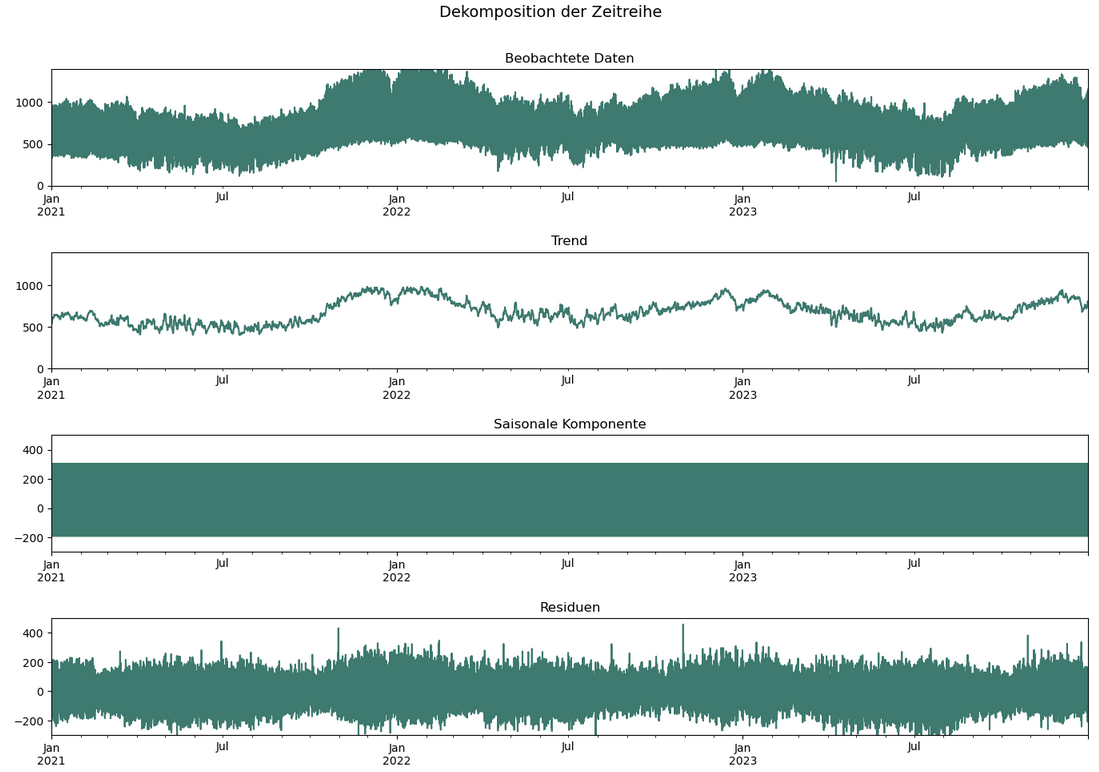
\includegraphics[width=13.25cm,keepaspectratio]{./images/Dekomposition_der_Zeitreihe_mit_Trend__S.png}
\caption{Dekomposition der Zeitreihe mit Trend, Saisonalität und Residuen}
\small~\textit{(Quelle: Eigene Darstellung).}
\label{fig:dekomposition_der_zeitreihe_mit_trend__saisonalitaet_und_residuen}
\end{figure}
\section{Ergebnisse der Transformer-Architektur mit unterschiedlicher Länge an historischen Daten}\label{sec:ergebnisse_der_transformer_architektur_mit_unterschiedlicher_laenge_an_historischen_daten}
Dieser Anhang zeigt eine erste Weiterführung der Ergebnisse aus \vref{subsubsec:transformer}, in dem die Transformer-Architektur mit historischen Daten über den Zeitraum Januar 2021 bis Dezember 2023 trainiert wurde.

Wie in der Diskussion angemerkt wurde, sollte für die Implementierung in eine reale Anwendung die Frage geklärt werden, wie viele historische Daten benötigt werden, ohne dass die Vorhersagegenauigkeit stark beeinträchtigt wird. Dieser Frage wurde in vorläufigen Tests nachgegangen, indem verschiedene Zeiträume als Eingabedaten in die in dieser Studie verwendete Transformer-Architektur eingegeben wurden. Dabei wurde die Vorhersagegenauigkeit für die 15-Minuten-Intervalle über 48 Stunden verglichen.

Bei der Modellkonfiguration die in Abbildung \ref{fig:transformer_ueber_48_stunden_mit_energieverbrauchsdaten_und_meteodaten_ueber_2_jahre_als_input} abgebildet ist, wurden Inputdaten von Januar 2022 bis Dezember 2023, 2 Jahre, verwendet. Die Auftrennung in Trainings- und Testdaten sowie alle restlichen Konfigurationen sind gleich geblieben. Die Fehlermetriken liegen für den MSE bei 6602.22 \(kW^{2}\), für den MAE bei 56.80 kW und für den RMSE bei 81.25 kW. Das Modell zeigt einen MAPE von 6.77 \%. Der MAPE-Wert liegt somit ungefähr um 2.8 \% über dem Wert aus der Modellkonfiguration mit Inputdaten von Januar 2021 bis Dezember 2023.


\begin{figure}[h!]
\centering
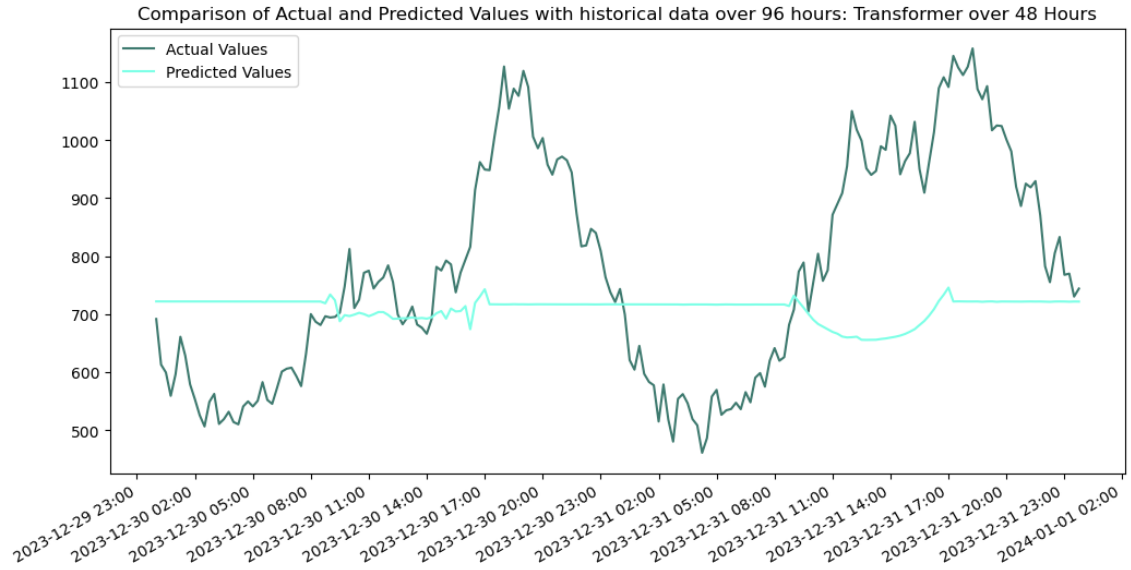
\includegraphics[width=12.75cm,keepaspectratio]{./images/Transformer_ueber_48_Stunden_mit_Energie.png}
\caption{Transformer über 48 Stunden mit Energieverbrauchsdaten und Meteodaten über 2 Jahre als Input}
\small~\textit{(Quelle: Eigene Darstellung).}
\label{fig:transformer_ueber_48_stunden_mit_energieverbrauchsdaten_und_meteodaten_ueber_2_jahre_als_input}
\end{figure}
Bei der Modellkonfiguration, die in Abbildung \ref{fig:transformer_ueber_48_stunden_mit_energieverbrauchsdaten_und_meteodaten_ueber_1_jahr_als_input} dargestellt ist, wurden Inputdaten von Januar 2023 bis Dezember 2023, 1 Jahr, verwendet. Die Auftrennung in Trainings- und Testdaten sowie alle restlichen Konfigurationen sind gleich geblieben. Die Fehlermetriken liegen für den MSE bei 6968.76 \(kW^{2}\), für den MAE bei 67.37 kW und für den RMSE bei 83.48 kW. Das Modell zeigt einen MAPE von 9.11 \%. Der MAPE-Wert liegt somit ungefähr um 5.2 \% über dem Wert aus der Modellkonfiguration mit Inputdaten von Januar 2021 bis Dezember 2023.


\begin{figure}[h!]
\centering
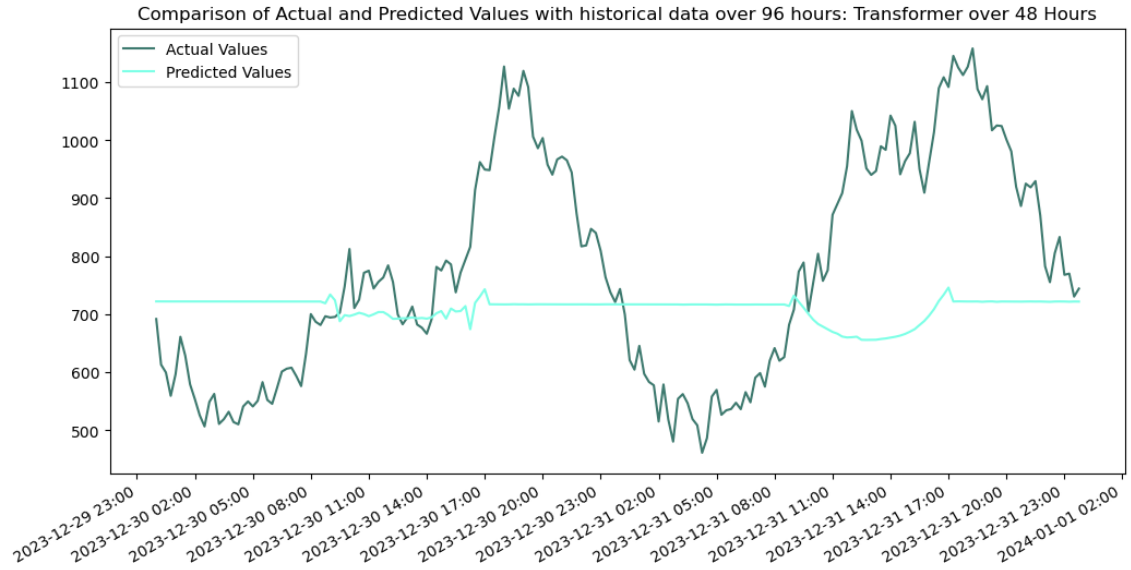
\includegraphics[width=12.75cm,keepaspectratio]{./images/Transformer_ueber_48_Stunden_mit_Energie.png}
\caption{Transformer über 48 Stunden mit Energieverbrauchsdaten und Meteodaten über 1 Jahr als Input}
\small~\textit{(Quelle: Eigene Darstellung).}
\label{fig:transformer_ueber_48_stunden_mit_energieverbrauchsdaten_und_meteodaten_ueber_1_jahr_als_input}
\end{figure}
Bei der Modellkonfiguration die in Abbildung \ref{fig:transformer_ueber_48_stunden_mit_energieverbrauchsdaten_und_meteodaten_ueber_6_monate_als_input} gezeigt ist, wurden Inputdaten der letzten 6 Monate aus dem Jahr 2023 verwendet, was 4464 Stunden entspricht. Die Auftrennung in Trainings- und Testdaten sowie alle restlichen Konfigurationen sind gleich geblieben. Die Fehlermetriken liegen für den MSE bei 7503.60 \(kW^{2}\), für den MAE bei 61.38 kW und für den RMSE bei 86.62 kW. Das Modell zeigt einen MAPE von 7.42 \%. Der MAPE-Wert liegt somit ungefähr um 3.5 \% über dem Wert aus der Modellkonfiguration mit Inputdaten von Januar 2021 bis Dezember 2023.

\begin{figure}[h!]
\centering
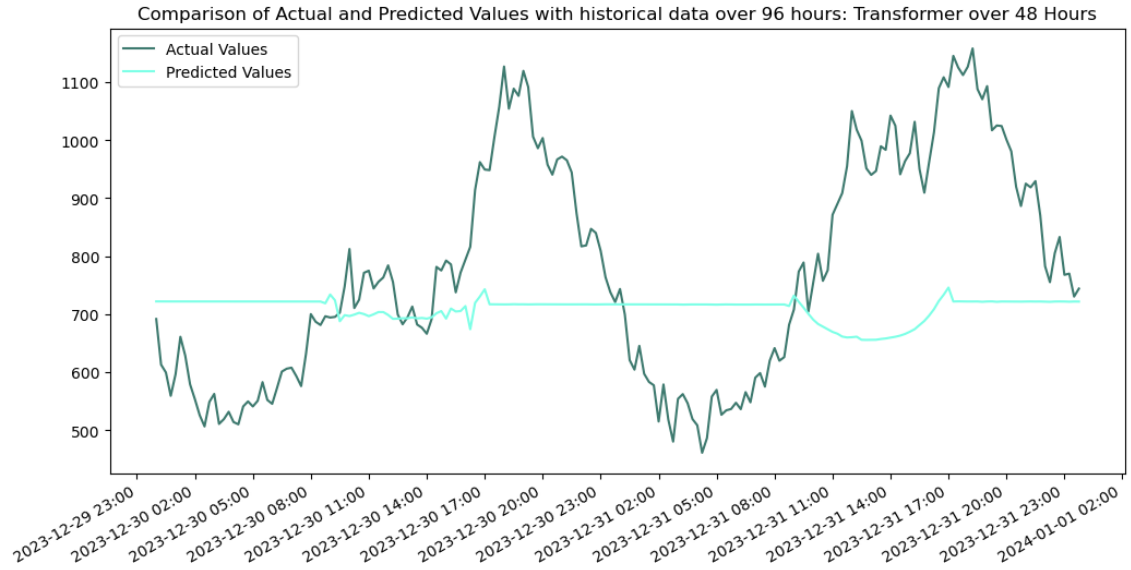
\includegraphics[width=12.75cm,keepaspectratio]{./images/Transformer_ueber_48_Stunden_mit_Energie.png}
\caption{Transformer über 48 Stunden mit Energieverbrauchsdaten und Meteodaten über 6 Monate als Input}
\small~\textit{(Quelle: Eigene Darstellung).}
\label{fig:transformer_ueber_48_stunden_mit_energieverbrauchsdaten_und_meteodaten_ueber_6_monate_als_input}
\end{figure}
Die nächste Modellkonfiguration verwendet Inputdaten der letzten 3 Monate aus dem Jahr 2023, was 2232 Stunden entspricht. Dieses Ergebnis ist in Abbildung \ref{fig:transformer_ueber_48_stunden_mit_energieverbrauchsdaten_und_meteodaten_ueber_3_monate_als_input} abgebildet. Die Auftrennung in Trainings- und Testdaten sowie alle restlichen Konfigurationen sind gleich geblieben. Die Fehlermetriken liegen für den MSE bei 6513.79 \(kW^{2}\), für den MAE bei 55.30 kW und für den RMSE bei 80.71 kW. Das Modell zeigt einen MAPE von 6.58~\%. Der MAPE-Wert liegt somit ungefähr um 2.6 \% über dem Wert aus der Modellkonfiguration mit Inputdaten von Januar 2021 bis Dezember 2023.

\begin{figure}[h!]
\centering
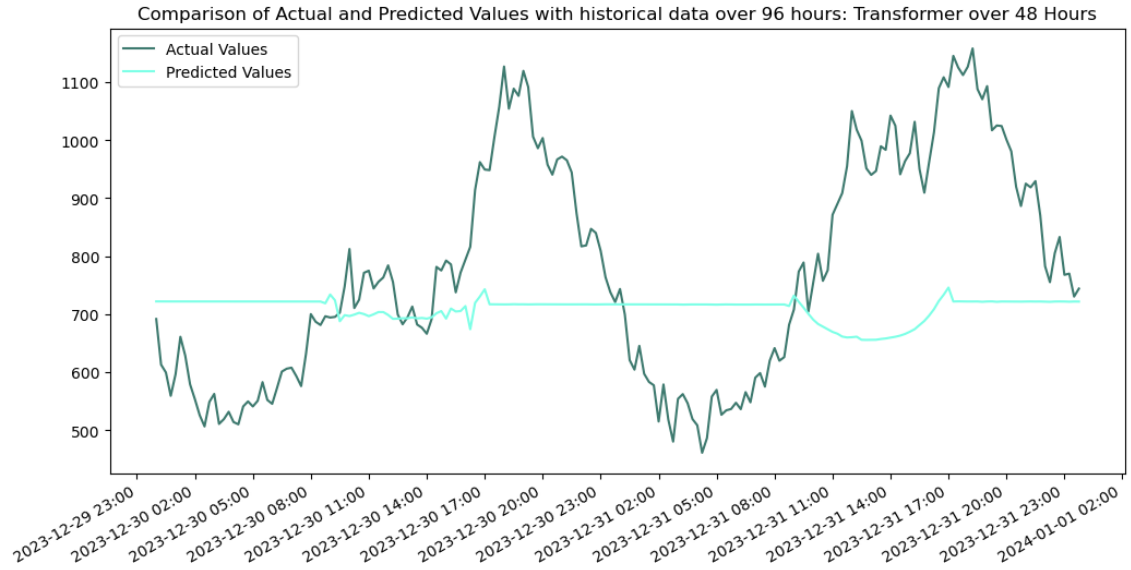
\includegraphics[width=12.75cm,keepaspectratio]{./images/Transformer_ueber_48_Stunden_mit_Energie.png}
\caption{Transformer über 48 Stunden mit Energieverbrauchsdaten und Meteodaten über 3 Monate als Input}
\small~\textit{(Quelle: Eigene Darstellung).}
\label{fig:transformer_ueber_48_stunden_mit_energieverbrauchsdaten_und_meteodaten_ueber_3_monate_als_input}
\end{figure}
Bei der Modellkonfiguration, die in Abbildung \ref{fig:transformer_ueber_48_stunden_mit_energieverbrauchsdaten_und_meteodaten_ueber_1_monat_als_input} dargestellt ist, wurden Inputdaten des letzten Monats aus dem Jahr 2023 verwendet, was 744 Stunden entspricht. Die Auftrennung in Trainings- und Testdaten sowie alle restlichen Konfigurationen sind gleich geblieben. Die Fehlermetriken liegen für den MSE bei 16'993.00 \(kW^{2}\), für den MAE bei 100.06~kW und für den RMSE bei 130.36 kW. Das Modell zeigt einen MAPE von 12.02 \%. Der MAPE-Wert liegt somit ungefähr um 8 \% über dem Wert aus der Modellkonfiguration mit Inputdaten von Januar 2021 bis Dezember 2023.

\begin{figure}[h!]
\centering
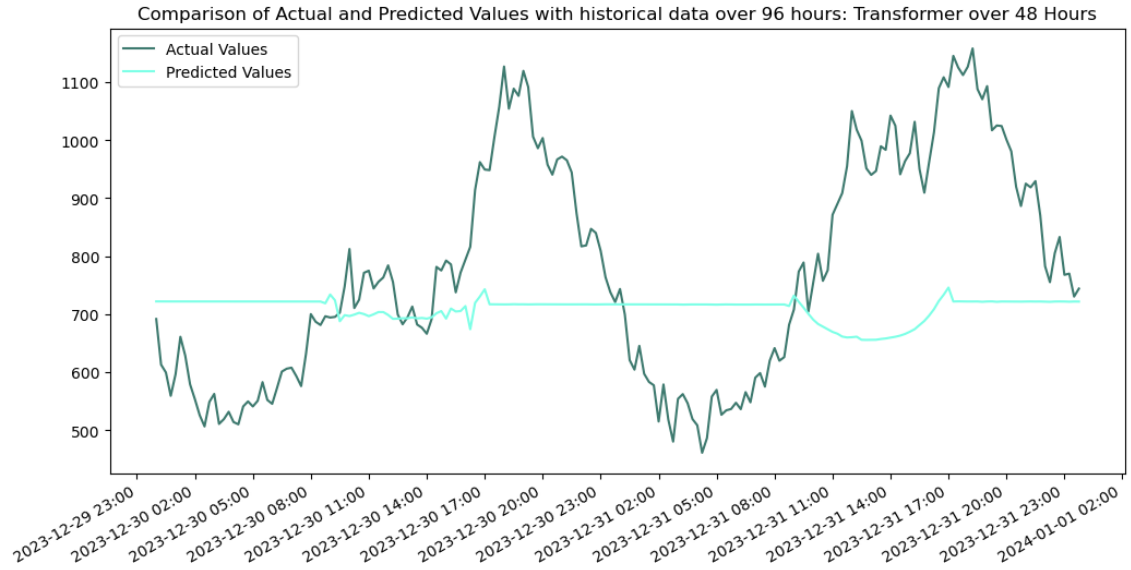
\includegraphics[width=12.75cm,keepaspectratio]{./images/Transformer_ueber_48_Stunden_mit_Energie.png}
\caption{Transformer über 48 Stunden mit Energieverbrauchsdaten und Meteodaten über 1 Monat als Input}
\small~\textit{(Quelle: Eigene Darstellung).}
\label{fig:transformer_ueber_48_stunden_mit_energieverbrauchsdaten_und_meteodaten_ueber_1_monat_als_input}
\end{figure}
Die nächste Modellkonfiguration nutzt Inputdaten der letzten 14 Tage aus dem Jahr 2023, was 336 Stunden entspricht. Dieses Ergebnis zeigt die Abbildung \ref{fig:transformer_ueber_48_stunden_mit_energieverbrauchsdaten_und_meteodaten_ueber_2_wochen_als_input}. Die Auftrennung in Trainings- und Testdaten sowie alle restlichen Konfigurationen sind gleich geblieben. Die Fehlermetriken liegen für den MSE bei 33'256.30 \(kW^{2}\), für den MAE bei 153.79~kW und für den RMSE bei 182.36 kW. Das Modell zeigt einen MAPE von 20.71 \%. Der MAPE-Wert liegt somit ungefähr um 17 \% über dem Wert aus der Modellkonfiguration mit Inputdaten von Januar 2021 bis Dezember 2023.

\begin{figure}[h!]
\centering
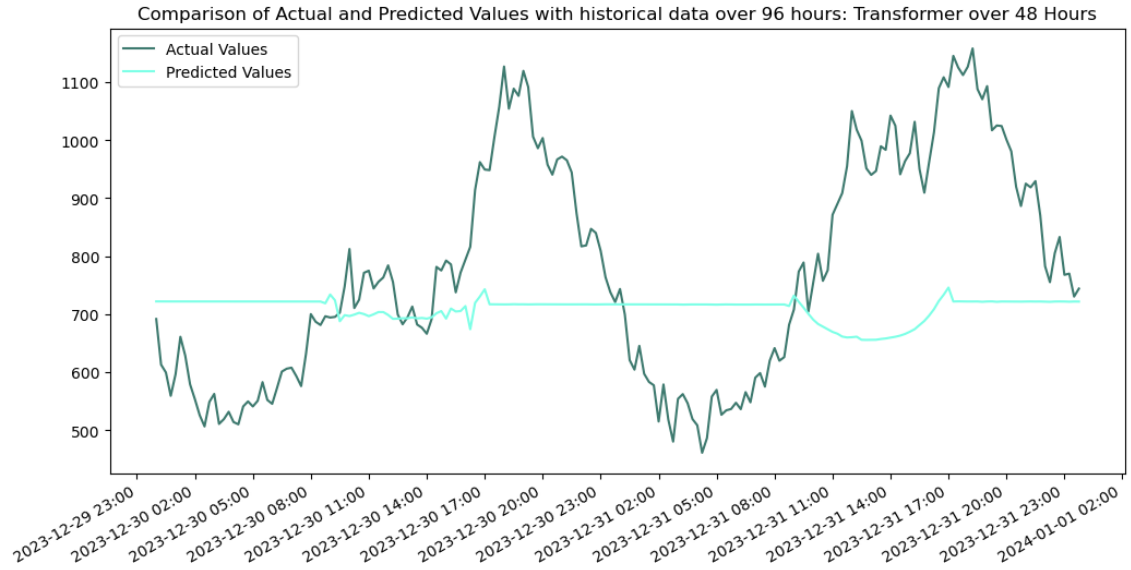
\includegraphics[width=12.75cm,keepaspectratio]{./images/Transformer_ueber_48_Stunden_mit_Energie.png}
\caption{Transformer über 48 Stunden mit Energieverbrauchsdaten und Meteodaten über 2 Wochen als Input}
\small~\textit{(Quelle: Eigene Darstellung).}
\label{fig:transformer_ueber_48_stunden_mit_energieverbrauchsdaten_und_meteodaten_ueber_2_wochen_als_input}
\end{figure}
Bei der Modellkonfiguration, die in Abbildung \ref{fig:transformer_ueber_48_stunden_mit_energieverbrauchsdaten_und_meteodaten_ueber_6_tage_als_input} abgebildet ist, wurden Inputdaten der letzten 6 Tage aus dem Jahr 2023 verwendet, was 144 Stunden entspricht. Die Auftrennung in Trainings- und Testdaten sowie alle restlichen Konfigurationen sind gleich geblieben. Die Fehlermetriken liegen für den MSE bei 19'753.72 \(kW^{2}\), für den MAE bei 109.81~kW und für den RMSE bei 140.55 kW. Das Modell zeigt einen MAPE von 13.16 \%. Der MAPE-Wert liegt somit ungefähr um 9 \% über dem Wert aus der Modellkonfiguration mit Inputdaten von Januar 2021 bis Dezember 2023.

\begin{figure}[h!]
\centering
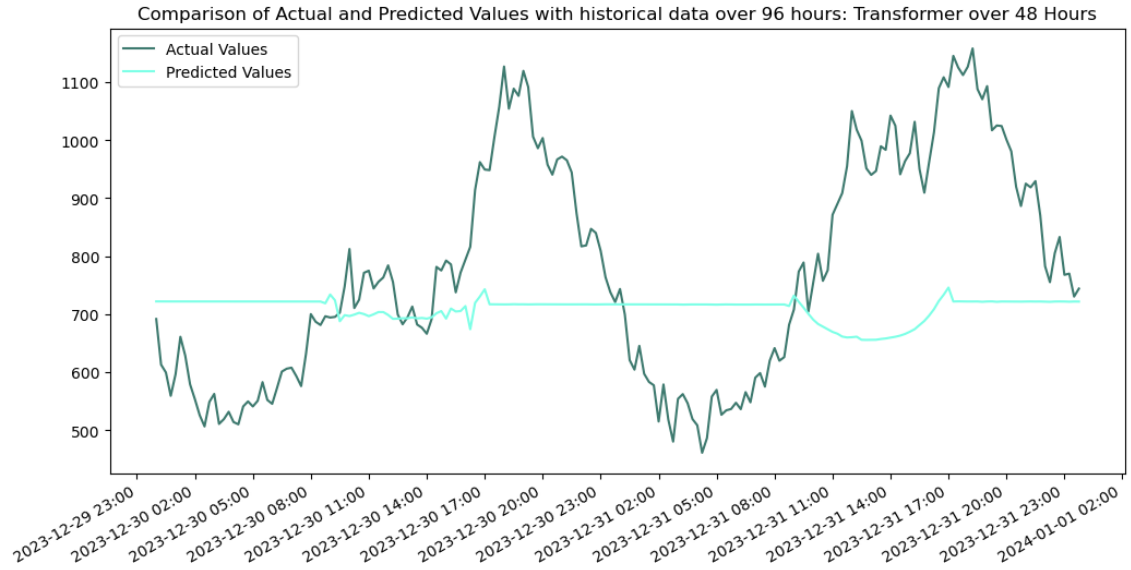
\includegraphics[width=12.75cm,keepaspectratio]{./images/Transformer_ueber_48_Stunden_mit_Energie.png}
\caption{Transformer über 48 Stunden mit Energieverbrauchsdaten und Meteodaten über 6 Tage als Input}
\small~\textit{(Quelle: Eigene Darstellung).}
\label{fig:transformer_ueber_48_stunden_mit_energieverbrauchsdaten_und_meteodaten_ueber_6_tage_als_input}
\end{figure}
Die letzte Modellkonfiguration hat Inputdaten der letzten 4 Tage aus dem Jahr 2023 verwendet, was 96 Stunden entspricht. Das Ergebnis ist in Abbildung \ref{fig:transformer_ueber_48_stunden_mit_energieverbrauchsdaten_und_meteodaten_ueber_4_tage_als_input} abgebildet. Die Auftrennung in Trainings- und Testdaten sowie alle restlichen Konfigurationen sind gleich geblieben. Die Fehlermetriken liegen für den MSE bei 42'016.49 \(kW^{2}\), für den MAE bei 170.67 kW und für den RMSE bei 204.98 kW. Das Modell zeigt einen MAPE von 21.66~\%. Der MAPE-Wert liegt somit ungefähr um 18 \% über dem Wert aus der Modellkonfiguration mit Inputdaten von Januar 2021 bis Dezember 2023.

\begin{figure}[h!]
\centering
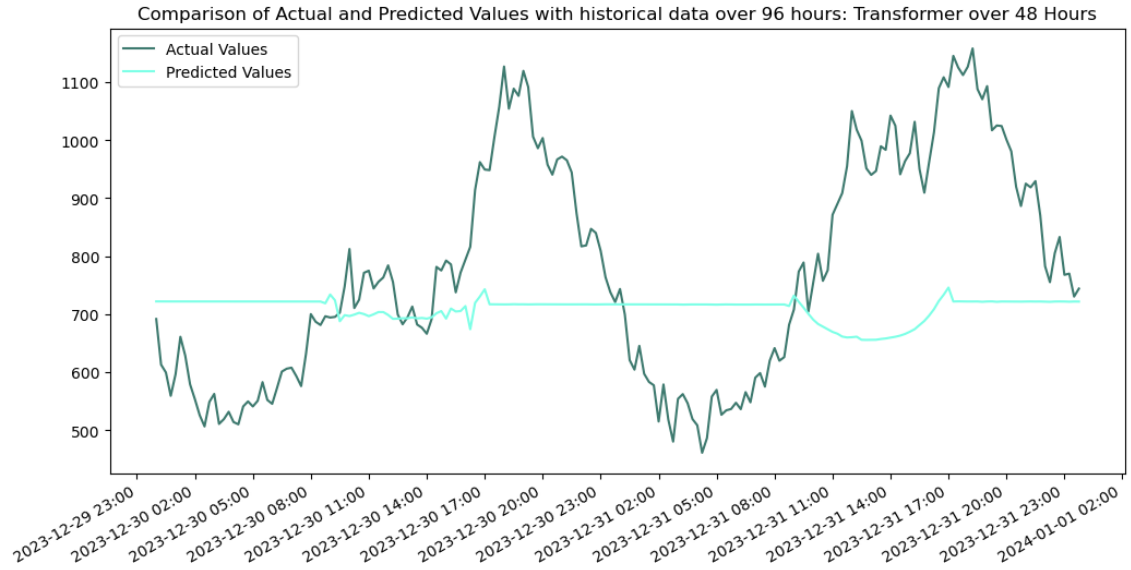
\includegraphics[width=12.75cm,keepaspectratio]{./images/Transformer_ueber_48_Stunden_mit_Energie.png}
\caption{Transformer über 48 Stunden mit Energieverbrauchsdaten und Meteodaten über 4 Tage als Input}
\small~\textit{(Quelle: Eigene Darstellung).}
\label{fig:transformer_ueber_48_stunden_mit_energieverbrauchsdaten_und_meteodaten_ueber_4_tage_als_input}
\end{figure}
Abschliessend lässt sich sagen, dass die Ergebnisse dieser ersten Tests zeigen, dass der Input an historischen Daten über mindestens 3 Monate hinweg notwendig ist, um einen MAPE von unter 10 \% zu erreichen. Weiter zeigen die beiden Modellkonfigurationen mit Inputdaten der letzten 3 Monate (MAPE: 6.58 \%) sowie der letzten 2 Jahre (MAPE: 6.77~\%) den niedrigsten MAPE und erreichen somit die beste Vorhersagegenauigkeit. Keine der Modellkonfigurationen erreicht einen gleich tiefen MAPE, wie wenn historische Daten über 3 Jahre hinweg als Inputdaten mitgegeben werden. In den Visualisierungen sind zudem Abweichungen von blossem Auge sichtbar, insbesondere in den zweiten 24 Stunden zwischen 11.00 Uhr und 18.00 Uhr.

\section{Ergebnisse der linearen Regression mit zeitbezogenen Variablen}\label{sec:ergebnisse_der_linearen_regression_mit_zeitbezogenen_variablen}
Dieser Anhang zeigt eine vorläufige Testdurchführung der linearen Regression mit zwei zusätzlichen zeitbezogenen Variablen als Input. In der Diskussion wurde angemerkt, dass in zukünftigen Forschungsrichtungen weitere zeitbezogene Variablen die Vorhersagegenauigkeit verbessern könnten.

Bei dieser Durchführung wurden zusätzlich zu den Energieverbrauchsdaten die beiden Variablen 'Hour' sowie 'DayOfWeek' als Input ergänzt. Die Auftrennung in Trainings- und Testdaten sowie alle restlichen Konfigurationen sind gleich geblieben. Der MAPE-Wert liegt bei 14.09 \%. In \vref{subsubsec:lineare_regression} erreichte die Modellkonfiguration einen MAPE von 19.29 \%. Auch in der Visualisierung \ref{fig:lineare_regression_ueber_48_stunden_mit_energieverbrauchsdaten_und_2_zeitbezogenen_features_als_inpu} ist die verbesserte Genauigkeit zu erkennen, da zumindest die Spitzen und Senken ansatzweise dargestellt sind. Dieses Testergebnis scheint darauf hinzuweisen, dass zeitbezogene Variablen die Vorhersagegenauigkeit, insbesondere von statistischen Modellen, verbessern können.


\begin{figure}[h!]
\centering
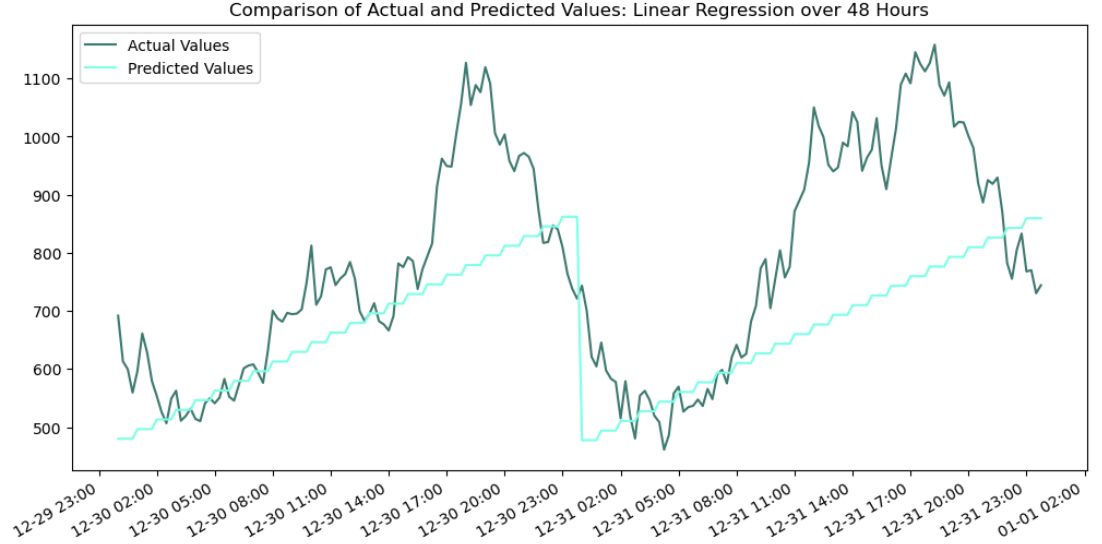
\includegraphics[width=13.25cm,keepaspectratio]{./images/Lineare_Regression_ueber_48_Stunden_mit_.png}
\caption{Lineare Regression über 48 Stunden mit Energieverbrauchsdaten und 2 zeitbezogenen Features als Input}
\small~\textit{(Quelle: Eigene Darstellung).}
\label{fig:lineare_regression_ueber_48_stunden_mit_energieverbrauchsdaten_und_2_zeitbezogenen_features_als_inpu}
\end{figure}
\newpage
\section{Verwendung von KI-gestützten Tools}\label{sec:verwendung_von_ki_gestuetzten_tools}
\textbf{ChatGPT Open AI}

\begin{center}
\footnotesize
\begin{longtable}{|p{2.1cm}|p{1.8cm}|p{9.7cm}|}
\hline
S.8 Zeile 15 - S.8 Zeile 36 & Paraphrasiert aus ChatGPT Open AI (15.03.2024). & Prompt: Fasse mir die wichtigsten Punkte aus diesem Artikel (hochgeladenes PDF) zusammen und erkläre mir die verwendeten Methoden auf Wirtschaftsinformatikniveau:

Hochgeladenes PDF: Machine Learning, Deep Learning and Statistical Analysis for forecasting building energy consumption — A systematic review \cite{ArticleMLDLSystematicReview}. Siehe \cite{ChatGPTArticleMLDLSystemicReviewSummary}
 \\
\hline
S.10 Zeile 81 - S.11 Zeile 7 & Paraphrasiert aus ChatGPT Open AI (15.03.2024). & Prompt: Fasse mir die wichtigsten Punkte aus diesem Artikel (hochgeladenes PDF) zusammen und erkläre mir die verwendeten Methoden auf Wirtschaftsinformatikniveau:

Hochgeladenes PDF: Deep learning and transfer learning models of energy consumption forecasting for a building with poor information data \cite{ArticleDLPoorData}. Siehe \cite{ChatGPTArticleDLPoorDATASummary}
 \\
\hline
S.21 Zeile 8  - S.21 Zeile 26 & Paraphrasiert aus ChatGPT Open AI (05.05.2024). & Prompt: Ich verwende die LSTM-Architektur (siehe angehängte Grafik). Diese ist angelehnt an folgenden Artikel: \href{https://www.pluralsight.com/resources/blog/guides/introduction-to-lstm-units-in-rnn}{https://www.pluralsight.com/resources/blog/guides/introduction-to-lstm-units-in-rnn}. Erkläre mir aus einer technischen Perspektive, in welcher Komponente was passiert. Siehe \cite{ChatGPTLSTMArchitecture} \\
\hline
S.22 Zeile 18 - S.23 Zeile 18 & Paraphrasiert aus ChatGPT Open AI (05.05.2024). & Prompt: Ich verwende die Transformer-Architektur (siehe angehängte Grafik). Diese ist angelehnt an folgenden Artikel: : \href{https://medium.com/@tech-gumptions/transformer-architecture-simplified-3fb501d461c8}{https://medium.com/@tech-gumptions/transformer-architecture-simplified-3fb501d461c8}. Erkläre mir aus einer technischen Perspektive, in welcher Komponente was passiert. Siehe \cite{ChatGPTTransformerArchitecture} \\
\hline
S.33 Zeile  6 - S.33 Zeile 9 & Paraphrasiert aus ChatGPT Open AI (27.04.2024). & Prompt:  Das sind meine Ressourcen, die mir für die Anwendung von Machine Learning zur Verfügung stehen. Beschreibe mir,  welche Ressource wofür ist und was zu den Ressourcen wichtig zu wissen ist: 1) Ubuntu-basierte Maschine, 2) AMD EPYC 7313P 16-Core Prozessor, 3) 146 GB Arbeitsspeicher, 4) Swap-Speicher beträgt 2 GB, 5) 2 NVIDIA A100 80GB PCIe Grafikkarten mit der neuesten CUDA-Version 12.4, 6) Jede GPU verfügt über 80 GB dedizierten Speicher. Siehe \cite{ChatGPTRessourcenML} \\
\hline
S.39 Zeile 20 - S.39 Zeile 21

und 

S.40 Zeile 6 - S.40 Zeile 8

 & Paraphrasiert aus ChatGPT Open AI (27.04.2024). & Prompt: Ich verwende für mein LSTM-Modell, um Kurzzeitprognosen zu erstellen, diesen Code hier. Erkläre mir die technischen Grundlagen des nn.modules sowie die forward-Methode etwas genauer [Angefügter Python-Code des LSTM-Modells]. Siehe \cite{ChatGPTCodeLSTM} \\
\hline
S.42 Zeile 4 - S.42 Zeile 5

und 

S.42 Zeile 15 - S.42 Zeile 16

 & Paraphrasiert aus ChatGPT Open AI (27.04.2024). & Prompt: Ich verwende für mein Transformer-Modell, um Kurzzeitprognosen zu erstellen, diesen Code hier. Erkläre mir die technischen Grundlagen des nn.modules sowie die forward-Methode etwas genauer [Angefügter Python-Code des Transformer-Modells]. Siehe \cite{ChatGPTCodeTransformer} \\
\hline
\caption{Verwendung von KI-gestützten Tools}
\label{tab:KI Tools}\\
\end{longtable}
\end{center}
\end{document} 